\documentclass[12pt]{article} % -- letter, article, report, book, memoir
\usepackage{amsmath}
\usepackage{amssymb}
\usepackage{tikz}
\usepackage{graphicx}
\usepackage{hyperref}
\usepackage{fancyhdr}
\usepackage{pdfpages}
\usepackage{wrapfig}
\usepackage{physics}
\usepackage{dsfont}
\usepackage{listings}
\usepackage{algorithm}
\usepackage{graphics} 
\usepackage[noend]{algpseudocode}
%=====linear algebra and general math notations
\newcommand{\rr}{\mathbb{R}}
\newcommand{\zz}{\mathbb{Z}}
\newcommand{\nn}{\mathbb{N}}
\newcommand{\cc}{\mathbb{C}}
\newcommand{\M}{\mathcal{M}}
\newcommand{\ntoinf}[1]{\lim_{{#1}\rightarrow \infty}}
\newcommand{\re}{\mathrm{Re}}
\newcommand{\im}{\mathrm{Im}}
\newcommand{\infnorm}[1]{\norm{#1}_{\infty}}
\newcommand{\twonorm}[1]{\norm{#1}_{2}}
\newcommand{\onenorm}[1]{\norm{#1}_{1}}
\newcommand{\iprod}[1]{\langle #1 \rangle}
\newcommand{\generalmatrixA}{
	\begin{pmatrix}
		a_{11} & a_{12} & \cdots & a_{1n} \\
		a_{21} & a_{22} & \cdots & a_{2n} \\
		\vdots & \vdots & \ddots & \vdots \\
		a_{n1} & a_{n2} & \cdots & a_{nn} \\
	\end{pmatrix}
}
\makeatletter
\def\BState{\State\hskip-\ALG@thistlm}
\makeatother
%=====
%===== probability theory and random processes
\newcommand{\expect}[1]{\mathbb{E}\big[ {#1} \big]}
\newcommand{\cov}[1]{\mathbb{C}ov({#1})}
\newcommand{\pp}[1]{\mathbb{P}({#1})}
\newcommand{\variance}[1]{\mathbb{V}ar\big[{#1}\big]}
%=====
%===== PDE theory
\newcommand{\intervoo}[2]{(#1, #2)}
\newcommand{\intervcc}[2]{\big[ #1, #2\big]}
\newcommand{\pdx}[1]{\frac{\partial}{\partial {#1}}}
\newcommand{\pddx}[1]{\frac{\partial^2}{\partial {#1}^2}}
\newcommand{\uno}{\large \textcircled{\small{1}}}
\newcommand{\dos}{\large\textcircled{\small{2}}}
\newcommand{\tres}{\large\textcircled{\small{3}}}
\newcommand{\yonn}{\large\textcircled{\small{4}}} % 4 in Japanese
\newcommand{\cancels}[1]{\underbrace{#1}_\textrm{cancelled}}
\newcommand{\overcomment}[1]{\overbrace{}^{#1}}
\newcommand{\ka}{\kappa}
\newcommand{\ga}{\gamma}
\newcommand{\uu}[2]{U_{#1}^{#2}} % shorthand
\newcommand{\argmax}{\operatornamewithlimits{argmax}}
\newcommand{\argmin}{\operatornamewithlimits{argmin}}
\newcommand{\1}[1]{\mathds{1}\left[#1\right]}

% short hand
\newcommand{\eps}{\epsilon}
\newcommand{\sig}{\sigma}

\DeclareMathOperator{\arccosh}{arccosh}
\DeclareMathOperator{\arcsinh}{arcsinh}
\DeclareMathOperator{\arctanh}{arctanh}
\DeclareMathOperator{\arcsech}{arcsech}
\DeclareMathOperator{\arccsch}{arccsch}
\DeclareMathOperator{\arccoth}{arccoth} 
%=====
% citations and pics

\usepackage[utf8]{inputenc}
\usepackage{biblatex}

\addbibresource{sample.bib}
\usepackage{graphicx}
\usepackage[left]{lineno}
\lstset{
  basicstyle=\ttfamily,
  mathescape
}
%=====
\linenumbers
\author{Hongli Zhao}
\title{Spring 2021 Math 128B Reference Solutions}
\date{May 31st, 2021}
\newtheorem{theorem}{Theorem}[section]
\newtheorem{corollary}{Corollary}[theorem]
\newtheorem{lemma}[theorem]{Lemma}
% page style

\pagestyle{fancy}
\fancyhf{}
\rhead{Hongli Zhao}
\lhead{Math 128B: Spring 2021}
\rfoot{Page \thepage}



\begin{document}

\maketitle

\begin{abstract}
	Math 128B: Numerical Analysis at UC Berkeley is the second course in the Math 128 series of undergraduate-level numerical analysis. Topics of the second course include matrix algorithms and analysis, function approximations, introduction to numerical ODEs (initial-boundary value problems) and numerical PDEs, following the textbook \emph{Numerical Analysis, 10th Edition} by Burden \& Faires, with slight edits to problem statements. The Spring 2021 offering of the course was given by Prof. Olga Holtz and graduate teaching assistant Oliver Edtmair, managed and supported via online platform \href{https://piazza.com/}{Piazza} and \href{https://www.gradescope.com/}{Gradescope} by grader Hongli Zhao. Major programming tools used are MATLAB, Julia and Python. 
	
	This document includes all published official solutions written by Hongli Zhao and advised by Prof. Olga Holtz, with revisions and suggestions given by Oliver Edtmair. All proofs and numerical algorithms may not be included, and is available upon request. Comments, errata and suggestions are welcome, please send an email to \url{mailto:honglizhaobob@berkeley.edu}. This is an unofficial reference and is not a publication.
\end{abstract}


\section{Homework 1}
\subsection{Norm Verification}

(a) Verify that:
$$
	\norm{x}_3 := \bigg( \sum_{j=1}^n \abs{x_j}^3\bigg)^{1/3}, x\in \mathbb{C}^n
$$ defines a norm.

(b) Find pair of constants $0<c<C$ such that:
$$
	c\norm{x}_1 \le \norm{x}_3 \le C\norm{x}_1, \forall x\in \cc^n
$$ as proof that $\norm{\cdot}_3$ is equivalent to $\norm{\cdot}_1$.

\subsubsection{a}
To show a function is a norm, we need to show 3 things (here $X =\mathbb{C}^n$). 

1. $\norm{x+y}\le\norm{x}+\norm{y}$ for all $x,y\in X$.

2. $\norm{tx} = \abs{t}\norm{x}$ for all $x\in X$ and $\lambda\in \mathbb{C}$.

3. $\norm{x} \ge 0$ and $=0$ if and only if $x=0$.

More generally, we can show that $\norm{x}_p$ defines a norm for $p\in [1, \infty)$.

By definition:
$$
	\norm{x}_p = \sqrt[p]{\sum_{i=1}^{n}\abs{x_i}^p} \ge 0
$$ since we have absolute value on each $x_i$.

If $x=0$, $\norm{0}_p=0$. Now suppose $\norm{x}_p=0$, we have:
$$
	\sum_{i=1}^n\abs{x_i}^p = 0
$$ since $\abs{x_i}^p \ge 0$ for all $i$, this implies $\abs{x_i} =0$ for all $i$, which means $x_i = 0$ for all $i$. Then $x=0$.

Take $t\in\cc$, consider:
$$
	\norm{tx}_p = 
	\bigg(
	\sum_{1}^n\abs{tx_i}^p
	\bigg)^{1/p} = \bigg(
	\sum_{1}^n\abs{t}^p\abs{x_i}^p
	\bigg)^{1/p} = \bigg(\abs{t}^p
	\sum_{1}^n\abs{x_i}^p
	\bigg)^{1/p}
$$
$$
	= (\abs{t}^p)^{1/p}\cdot\bigg(\sum_1^n\abs{x_i}^p\bigg)^{1/p} = \abs{t}\cdot\norm{x}_p
$$

Triangle inequality follows from Minkowski inequality.

\subsubsection{b}
There is a functional analysis fact that in a finite dimensional vector space (such as $\cc^n$ here), all norms are equivalent (if interested, Chapter 5.1 Exercise 6 from \emph{Real Analysis: Modern Techniques and Their Applications} by Gerald Folland (or other standard functional analysis textbooks) provides a statement). 

Here we only apply this fact to our specific case $p=3$.

First:
$$
\norm{x}_3^3 = \sum_1^{n}\abs{x_i}^3 
$$ on the other hand:
$$
	\norm{x}_1^3 = \bigg(
	\sum_1^{n}\abs{x_i}
	\bigg)^3 = \sum_{1}^n\abs{x_i}^3 + 3\sum_{i<j}\abs{x_i}^2\abs{x_j} + 6\sum_{i<j<k}\abs{a_i}\abs{a_j}\abs{a_k}
$$ which is larger than:
$$
	\ge \sum_1^{n}\abs{x_i}^3  = \norm{x}_3^3
$$ therefore taking cube root on both sides, we showed:
$$
	\norm{x}_3 \le \norm{x}_1
$$ with constant 1.

For the other direction, consider:
$$
	\norm{x}_{\infty}^3 = \max_i\abs{x_i}^3 \le \sum_{1}^n\abs{x_i}^3 = \norm{x}_3^3
$$ on the other hand we have showed before (for all $i$, each $\abs{x_i}$ is less than the maximum element, then repeating the max $n$ times is going to be larger than adding all $\abs{x_i}$ together):
$$
	\norm{x}_1 \le n\norm{x}_{\infty}
$$ or:
$$
	\norm{x}^3_1 \le n^3\norm{x}^3_{\infty}
$$ combining the previous inequalities:
$$
	\frac{1}{n^3}\norm{x}_1^3\le\norm{x}_{\infty}^3\le \norm{x}_3^3
$$ we take cube root, and get:
$$
	\frac1n\norm{x}_1 \le \norm{x}_3
$$ here the constant is $1/n$. 

As above, we showed that $\norm{\cdot}_1$ is equivalent to $\norm{\cdot}_3$.



\newpage
\subsection{Plotting Unit Sphere for Different Norms}
Use MATLAB to plot the unit spheres for norms $\norm{\cdot}_1$ and $\norm{\cdot}_3$ in $\rr^3$.

\subsubsection{}
There are many ways to make the plot. The MATLAB code for this particular plot is below:
\begin{verbatim}
% plotting unit ball with respect to different norms

% sample from a Gaussian
X = randn(10000, 3);

% l1 norm coeffs
l1_coef = sum(abs(X).^1, 2).^(1/1); 
% l3 norm coeffs
l3_coef = sum(abs(X).^3, 2).^(1/3); 
% normalize data by p-norm 
X_l1_data = (bsxfun(@times, X, 1./l1_coef)); 
X_l3_data = (bsxfun(@times, X, 1./l3_coef)); 


figure; 
scatter3(X_l1_data(:, 1), X_l1_data(:, 2), X_l1_data(:, 3),...
    '*', "red"); 
hold on; 
scatter3(X_l3_data(:, 1), X_l3_data(:, 2), X_l3_data(:, 3),...
    'o', "blue"); title('comparison of unit closed ball for l^3 and l^1');
\end{verbatim} which yields the result:
\newpage
\begin{figure}[t]
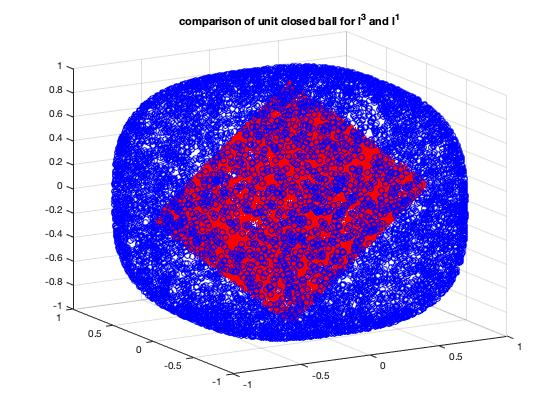
\includegraphics[width=12cm]{p2plot.jpg}
\centering
\end{figure}
\newpage


\subsection{Calculating 2-norm and $\infty$-norm}

For each of the matrices, find $\infty$-norm and 2-norm. 

(1)

$$
	\begin{pmatrix}
		1 & 2 \\
		3 & 2
	\end{pmatrix}
$$

(2)

$$
	\begin{pmatrix}
		-2 & 3 \\
		3 & -2
	\end{pmatrix}
$$

(3)

$$
	\begin{pmatrix}
		1 & 1 & 1 & 1 \\
		0 & 2 & 2 & 3 \\
		0 & 0 & 3 & 2 \\
		0 & 0 & 0 & 4
	\end{pmatrix}
$$

The matrix operator 2-norm is the square root of largest eigenvalue of $A^TA$ (for $A$ real), and the $l_{\infty}$-norm is given by the maximum absolute row sum.
\subsubsection{}
$$
	A = \begin{pmatrix}
	1 & 2\\
	3 & 2
	\end{pmatrix}, 
	A^TA = \begin{pmatrix}
	10 & 8\\
	8 & 8
	\end{pmatrix}
$$

$$
	\norm{A}_2 = \sqrt{\lambda_{max}(A^TA)} = \sqrt{9+\sqrt{65}}
$$ and:
$$
	\norm{A}_{\infty} = \max_{1\le i\le 2}\sum_{j=1}^2\abs{a_{ij}} = 5
$$



\subsubsection{}
$$
A = \begin{pmatrix}
	-2 & 3\\
	3 & -2
\end{pmatrix}, 
A^TA = 
\begin{pmatrix}
	13 & -12\\
	-12 & 13
\end{pmatrix}
$$

$$
	\norm{A}_2 = \sqrt{\lambda_{max}(A^TA)} = 5
$$
$$
	\norm{A}_{\infty} = 5
$$


\subsubsection{}
$$
A = \begin{pmatrix}
	1 & 1 & 1 & 1\\
	0 & 2 & 2 & 3\\
	0 & 0 & 3 & 2\\
	0 & 0 & 0 & 4
	\end{pmatrix},
	A^TA = 
	 \begin{pmatrix}
	1 & 1 & 1 & 1\\
	1 & 5 & 5 & 7\\
	1 & 5 & 14 & 13\\
	1 & 7 & 13 & 30
	\end{pmatrix}
$$ 

$$
\norm{A}_2\approx 6.2813
$$
$$
	\norm{A}_{\infty} = 7
$$

\newpage

\subsection{2-norm of Symmetric Matrix}
Show that if a matrix $A$ is symmetric, then its 2-norm is equal to its spectral radius.
\subsubsection{}
$A$ is symmetric, it admits the following decomposition:
$$
	A = PDP^{-1}
$$ where $P$ is orthogonal, thus:
$$
	A^TA = PDP^{-1}PDP^{-1} = PD^2P^{-1}
$$ then the eigenvalues of $A^TA$ are simply squares of the eigenvalues of $A$. Then:
$$
	\norm{A}_2 = \sqrt{\lambda_{max}(A^TA)} = \sqrt{\lambda_{max}(A)^2}  = \lambda_{max}(A) = \rho(A)
$$ as desired.


\newpage
\section{Homework 2}
\subsection{MATLAB implementation of Jacobi Method}
Please refer to Algorithm 7.1 and 7.2 for exact implementations. Regarding implementations:

1. Many students used for loops to find $L, U$, in MATLAB, we can consider using:
\begin{verbatim}
triu(A);

tril(A);
\end{verbatim} to get upper, lower triangular parts of $A$.

2. In practical implementations, we should avoid calling explicit inverse of matrices; rather, we should use a linear solver or backslash. Here is actually an interesting discussion that explores why this is the case:
\begin{verbatim}
https://arxiv.org/abs/1201.6035
\end{verbatim}

\subsection{MATLAB implementation of Gauss-Seidel Method}
Gauss-Seidel usually requires fewer iterations to reach  similar level of accuracy as Jacobi as it (GS) tries to incorporate new information at each equation in the linear system. If at the $n$-th equation we already have solutions for the previous $(n-1)$, why not use them in solving the current one?

Furthermore, the condition for convergence should be fulfilled for diagonally dominant matrices with any initial condition.

\subsection{Convergence of Matrix Powers}
Let A be a square matrix and let $\norm{\cdot}$ be any matrix norm (not necessarily natural/induced). Prove that $\lim_{k\rightarrow \infty}\norm{A^k} = 0$ if $\rho(A) < 1$.

\subsubsection{}
Suppose $\rho(A)<1$, we have $\ntoinf{n}\lambda_{i}^m = 0$ for all $i$. Any matrix $A$ admits a Jordan decomposition in the following form:
$$
	A = PJP^{-1}
$$ where $P$ is invertible, and $J$ is a block-diagonal matrix with $k \le n$ blocks. And each block $J_i$ for $i\in[1,k]$ have superdiagonal be all 1's, or:
$$
	J_i 
	=
	\begin{pmatrix}
		\lambda_i & 1 & & \\
		& \lambda_i & \ddots & \\
		& & \ddots & 1& \\
		& & & \lambda_i
	\end{pmatrix}
$$ and we can express:
$$
	J = 
	\begin{pmatrix}
		J_1 & & & & \\
		& J_2 & & & \\
		& & \ddots & & \\
		& & & J_{k-1} & \\
		& & & & J_k
	\end{pmatrix}
$$

Then we have:
$$
	A^m = (PJP^{-1})\cdot(PJP^{-1})\cdots (PJP^{-1}) = PJ^mP^{-1}
$$ and since $J$ is block-diagonal:
$$
	J^m = 
	\begin{pmatrix}
		J_1^m & & & & \\
		& J_2^m & & & \\
		& & \ddots & & \\
		& & & J_{k-1}^m & \\
		& & & & J_k^m
	\end{pmatrix}
$$ then we can investigate what each $J_i^m$ behavior is. 


For a Jordan matrix $J$ with eigenvalue $\lambda$, we can write it as:
$$
	J = (\lambda I + S)
$$ where $S$ is called a "shift" matrix, in the sense that it shifts all values in a vector up by 1 place, zeroing out the last element. More explicitly suppose we are in $\rr^d$:
$$
	S = 
	\begin{pmatrix}
		0 & 1 & & \\
		& 0 & \ddots & \\
		& & \ddots & 1& \\
		& & & 0
	\end{pmatrix}
$$ and the shifting is in the sense that:
$$
S\cdot [x_1, x_2,\cdots, x_{d-1}, x_d]^T = [x_2, x_3,\cdots, x_{d}, 0]^T
$$

Furthermore, $S$ and $\lambda I$ commutes, because $I$ is the identity. Then we can write the powers of $J$ as a binomial expansion:
$$
J^m = (\lambda I + S)^m = \sum_{0}^m {m\choose r}\lambda^{m-r}S^r
$$	

By the formulation of $S$, we know that it is nilpotent with degree $n$ (repeating $S$ by $n$ times on a vector, we get the 0 vector). Eigenvalues of nilpotent matrices can only be 0, therefore $S^r$ will not cause the norm to grow. 

Furthermore, $S^d$ becomes 0, and $d$ as the matrix dimension is finite. Then as $m\rightarrow\infty$, we can safely write:
$$
	\ntoinf{m}J^m = \sum_0^{d-1}\lambda^{m-r}S^r
$$ because all subsequent terms $S^d, S^{d+1},\cdots$ will be wiped out by the fact that $S^d = 0$. Therefore this is a finite matrix sum with $\lambda^{m-r}\rightarrow 0$ ($r$ can only grow as large as $d-1$). Thus we conclude:
$$
	\ntoinf{m}J^m = 0
$$ and this is true for all Jordan matrices with $\abs{\lambda}<1$. Therefore $J^m \rightarrow 0$ as $m\rightarrow \infty$.

Now we can use what we showed above and conclude:
$$
	\ntoinf{m}\norm{A^m} = \ntoinf{m}\norm{PJ^mP^{-1}} \le \ntoinf{m}\norm{P}\norm{P^{-1}}\norm{J^m} = \ka(P)\ntoinf{m}\norm{J^m} = 0
$$ here we use the fact that $\ka(P)$ is finite unless $P$ is singular (which by Jordan normal form, it is not), hence the last equality to 0.
\newpage
\section{Homework 3}
\subsection{Find the first two iterations of the SOR method}
Find the first two iterations of the SOR method with $\omega = 1.2$ for the following linear system:
$$
	10x_1 - x_2 = 9
$$
$$
	-x_1 + 10x_2 - 2x_3 = 7
$$
$$
	-2x_2 + 10x_3 = 6
$$ check convergence of the corresponding $T_{\omega}$ matrix.

\subsubsection{}
The linear system is:
$$
	\begin{pmatrix}
		10 & -1 & 0 \\
		-1 & 10 & -2 \\
		0 & -2  & 10
	\end{pmatrix}x =
	\begin{pmatrix}
		9 \\
		7\\
		6
	\end{pmatrix}
$$ or $Ax= b$.

In SOR, the matrix $A$ permits the following decomposition:
$$
	A = D + L + U
$$ where:
$$
	D = \begin{pmatrix}
		10 & 0 & 0 \\
		0 & 10 & 0 \\
		0 & 0  & 10
	\end{pmatrix}, 
	U = 
	\begin{pmatrix}
		0 & -1 & 0 \\
		0 & 0 & -2 \\
		0 & 0  & 0
	\end{pmatrix}, 
	L = \begin{pmatrix}
		0 & 0 & 0 \\
		-1 & 0 & 0 \\
		0 & -2  & 0
	\end{pmatrix}
$$

The exact solution for this linear system can be calculated by hand or a calculator:
$$
	x = \begin{pmatrix}
		\frac{473}{475} \\
		\frac{91}{95}\\
		\frac{375}{475}
	\end{pmatrix} 
	\approx
	[0.99578947, 0.95789474, 0.79157895]^T
$$

See textbook equation (7.18). The matrix $T_{w}$ is given by:
$$
	T_{w} = (D - wL)^{-1}\big[
	(1-w)D + wU
	\big]
$$ letting $w=1.2$ will yield approximately:
$$
	T_{w} = 
	\begin{pmatrix}
		-0.2 & -0.12 & 0 \\
		0.024 & -0.1856 & -0.24 \\
		-0.00576 & 0.044544  & -0.1424
	\end{pmatrix}
$$

In line with B\&F Definition 7.16, it is enough to check the spectral radius of $T_w$, namely:
$$
	\rho(T_w) = \max\abs{\lambda(T_w)} \le \norm{T_w} \approx 0.4115
$$ (one can also choose to compute the eigenvalues, or check positive-definiteness. Therefore the matrix is convergent, refer to Theorem 7.17 for detailed properties.

Now we use $T_w$ to perform two iterations of SOR, exact details are skipped, follow:
$$
	x^{(k)} = T_wx^{(k-1)} + c_w
$$ where $c_w = w(D-wL)^{-1}b$. 

$$
	c_w \approx
	\begin{pmatrix}
		1.08 \\
		0.7104\\
		0.549504
	\end{pmatrix}
$$

Pick initial guess $x^{(0)} = [1,1,1]^T$ (it is okay to choose other initial guesses, correctness was graded based on values for $T_w, c_w$). Two steps of SOR yields:
$$
	x^{(1)} = T_wx^{(0)} + c_w = 
	\begin{pmatrix}
		0.76 \\
		0.3088\\
		0.445888
	\end{pmatrix}
$$

$$
	x^{(2)} = T_wx^{(1)} + c_w = 
	\begin{pmatrix}
		0.890944 \\
		0.5643136\\
		0.49538714
	\end{pmatrix}
$$



\newpage
\subsection{Inequality}
Let $\ka(A)$ denote the condition number of square matrix $A$. Show that any singular matrix $B$ satisfies the following inequality:
$$
	\ka(A)^{-1} \le \frac{\norm{A-B}}{\norm{A}}
$$

\subsubsection{}


$B$ is singular, therefore $ker(B) \neq \emptyset$, pick any $x\in ker(B)$, assume $\norm{x} = 1$ (if not, normalize by $x' = x/\norm{x}$). Then we observe:
$$
	(A- B)x = Ax-Bx = Ax
$$

Then we have:
$$
	\norm{Ax} = \norm{(A-B)x} \le \norm{A-B}\norm{x} = \norm{A-B}
$$

As we learned in class:
$$
	\ka(A) = \norm{A}\cdot\norm{A^{-1}}
$$ 

It is enough to show $\norm{A-B}\cdot \norm{A^{-1}} \ge 1$ (rearrange the original inequality).

Consider the matrix-vector multiply:
$$
	A^{-1}(A-B)x= Ix - A^{-1}Bx = x
$$ recall $Bx = 0$. Then we have:
$$
	1=\norm{x} = \norm{A^{-1}(A-B)x} \le \norm{A^{-1}}\norm{A-B}\norm{x} = \norm{A^{-1}}\norm{A-B}
$$ as desired.








\newpage
\subsection{Gaussian elimination with three-digit rounding}
Use Gaussian elimination and three-digit rounding arithmetic to find an approximate solution to the following linear system:
$$
	0.03x_1 + 58.9x_2 = 59.2
$$
$$
	5.31x_1 - 6.1x_2 = 47.0
$$
	
Then use one iteration of iterative refinement. Compare both approximations to the
exact solution.

\subsubsection{}
We have the system:
$$
	\begin{pmatrix}
		0.03 & 58.9 \\
		5.31 & -6.1 \\
	\end{pmatrix}x =
	\begin{pmatrix}
		59.2 \\
		47.0
	\end{pmatrix}
$$ the system has an exact solution:
$$
	x = 
	\begin{pmatrix}
		10.0 \\
		1.0
	\end{pmatrix}
$$ the key is to understand how 3-digit rounding may give poor accuracy. Let $r_1, r_2$ denote row 1 and row 2 of the matrix, the Gaussian Elimination step is to add $-\frac{5.31}{0.03}r_1$ to $r_2$. Here we have:
$$
-\frac{5.31}{0.03}\approx -177
$$ since we only have 3 digits. Doing this calculation by hand:
$$
	-\frac{5.31}{0.03}r_1 = -5.31x_{1} - 10400x_{2} = -10300
$$

Now add this to $r_2$ we have:
$$
	-10400x_2 = -10300
$$ then solve, and round by 3 digits:
$$
	\tilde{x}_2 = 0.990
$$

This causes problems, plug $\tilde{x}_2$ back to $r_1$ and solve for $x_1$ we have:
$$
	\tilde{x}_1 = \frac{59.2 - 58.9 \cdot 0.990}{0.03} \approx \frac{0.900}{0.03} = 30.0
$$

The reason why this happens is because $A$ is ill-conditioned (Definition 7.28). 
$$
	\ka(A)_{\infty} \approx 12.24
$$


Now keeping 3-digit rounding, we use one step of iterative refinement. We had:
$$
	x^{(1)} =\tilde{x}= 
	\begin{pmatrix}
		30.0\\
		0.990
	\end{pmatrix}
$$ which yields residual:
$$
	r^{(1)} = b-Ax^{(1)} = 
	\begin{pmatrix}
		59.2 \\
		47.0
	\end{pmatrix}-\begin{pmatrix}
		0.03 & 58.9 \\
		5.31 & -6.1 \\
	\end{pmatrix}\begin{pmatrix}
		30.0\\
		0.990
	\end{pmatrix}
$$ in more detail:
$$
	0.03 \times 30.0 + 58.9 \times 0.990 \approx 0.900 + 58.3 \approx 59.2
$$
$$
	5.31 \times 30.0 -6.1 \times 0.990 \approx 159 - 6.04 \approx 153
$$
$$
	r^{(1)}\approx 
	\begin{pmatrix}
		59.2 \\
		47.0
	\end{pmatrix}-\begin{pmatrix}
		59.2\\
		153
	\end{pmatrix} = 
	\begin{pmatrix}
		0\\
		-106
	\end{pmatrix}
$$

Now solve for the correction:
$$
	A\delta^{(1)} = r^{(1)}
$$ yielding:
$$
	\delta^{(1)} \approx 
	\begin{pmatrix}
		-20.0\\
		0.0102
	\end{pmatrix}
$$ 

Refine our solution:
$$
	x^{(2)} = x^{(1)} + \delta^{(1)} = \begin{pmatrix}
		30.0\\
		0.990
	\end{pmatrix}+
	\begin{pmatrix}
		-20.0\\
		0.0102
	\end{pmatrix} =
	\begin{pmatrix}
		10.0\\
		1.00
	\end{pmatrix}
$$ which is much better!





\newpage
\subsection{Perturbation Estimate}
Let:
$$
	A = 
	\begin{pmatrix}
		1 & 2 \\
		1.00001 & 2
	\end{pmatrix}, b = 
	\begin{pmatrix}
		3 \\
		3.00001
	\end{pmatrix}
$$

The problem $Ax = b$ has exact solution $x = [1,1]^T$. Use seven-digit rounding arithmetic to solve the perturbed system with:
$$
	\tilde{A} = 
	\begin{pmatrix}
		1 & 2 \\
		1.000011 & 2
	\end{pmatrix}, \tilde{b} =
	\begin{pmatrix}
		3.00001 \\
		3.00003
	\end{pmatrix}
$$ and compare the actual error to the Perturbation Estimate.

\subsubsection{}
We have exact system:
$$
	A = 
	\begin{pmatrix}
		1 & 2 \\
		1.00001 & 2 \\
	\end{pmatrix},
	b =
	\begin{pmatrix}
		3\\
		3.00001
	\end{pmatrix}
$$ and it is perturbed with (follow the notation from B\&F Theorem 7.29):
$$
	\delta A =
	\begin{pmatrix}
		0 & 0 \\
		0.000001 & 0 \\
	\end{pmatrix},
	\delta b =
	\begin{pmatrix}
		0.00001\\
		0.00002
	\end{pmatrix},
	\tilde{A} = A+\delta A, \tilde{b} = b+\delta b
$$

Then with 7-digit rounding:
$$
	\tilde{x} \approx 
	\begin{pmatrix}
		1.8181820\\
		0.5909141
	\end{pmatrix}
$$

Refer to Formula (7.25) for the perturbation bound (with respect to inf norm):
$$
	LHS = \frac{\norm{x - \tilde{x}}}{\norm{x}} \approx 0.82
$$

$$
	RHS = 
	\frac{\ka(A)\norm{A}}{\norm{A} - \ka(A)\norm{\delta A}}\cdot\bigg(
	\frac{\norm{\delta b}}{\norm{b}}+\frac{\norm{\delta A}}{\norm{A}}
	\bigg) \approx 5.25
$$ which is what's expected since:
$$
	\norm{\delta A} = 10^{-6}
$$ but:
$$
	\frac{1}{\norm{A^{-1}}}\approx 5\times 10^{-6} > \norm{\delta A}
$$

Full credit for this question was given if student has written the correct formula for the error upper bound and made reasonable attempt to evaluate it (exact number does not have to be meticulously matched), and has correctly computed $\delta A,\delta b$. The error bound should be on the order of $O(10^{-5})$. The perturbed solution was more rigorously checked.

\newpage



%===== begin hw 4
\section{Homework 4}
\subsection{Implement CG Method}
Create a function with inputs matrix $A$, vector $b$, $x^{(0)}$ as initial guess and tolerance $tol$. The algorithm implements conjugate gradient method and should find an approximate solution to $Ax = b$ without preconditioning. CG should terminate after $n$ steps. Run your algorithm with test linear systems.

\subsubsection{}
Example implementation in Python and Julia are as follows, with very simple test with:
$$
A =\begin{pmatrix}
	4 & 1\\
	1 & 3
\end{pmatrix}, b=
\begin{pmatrix}
	1 \\
	2
\end{pmatrix}
$$ (it is a very good idea to try translating the code to MATLAB if you are not familiar with the algorithm, MATLAB code was intentionally not provided).


Python version (next page):
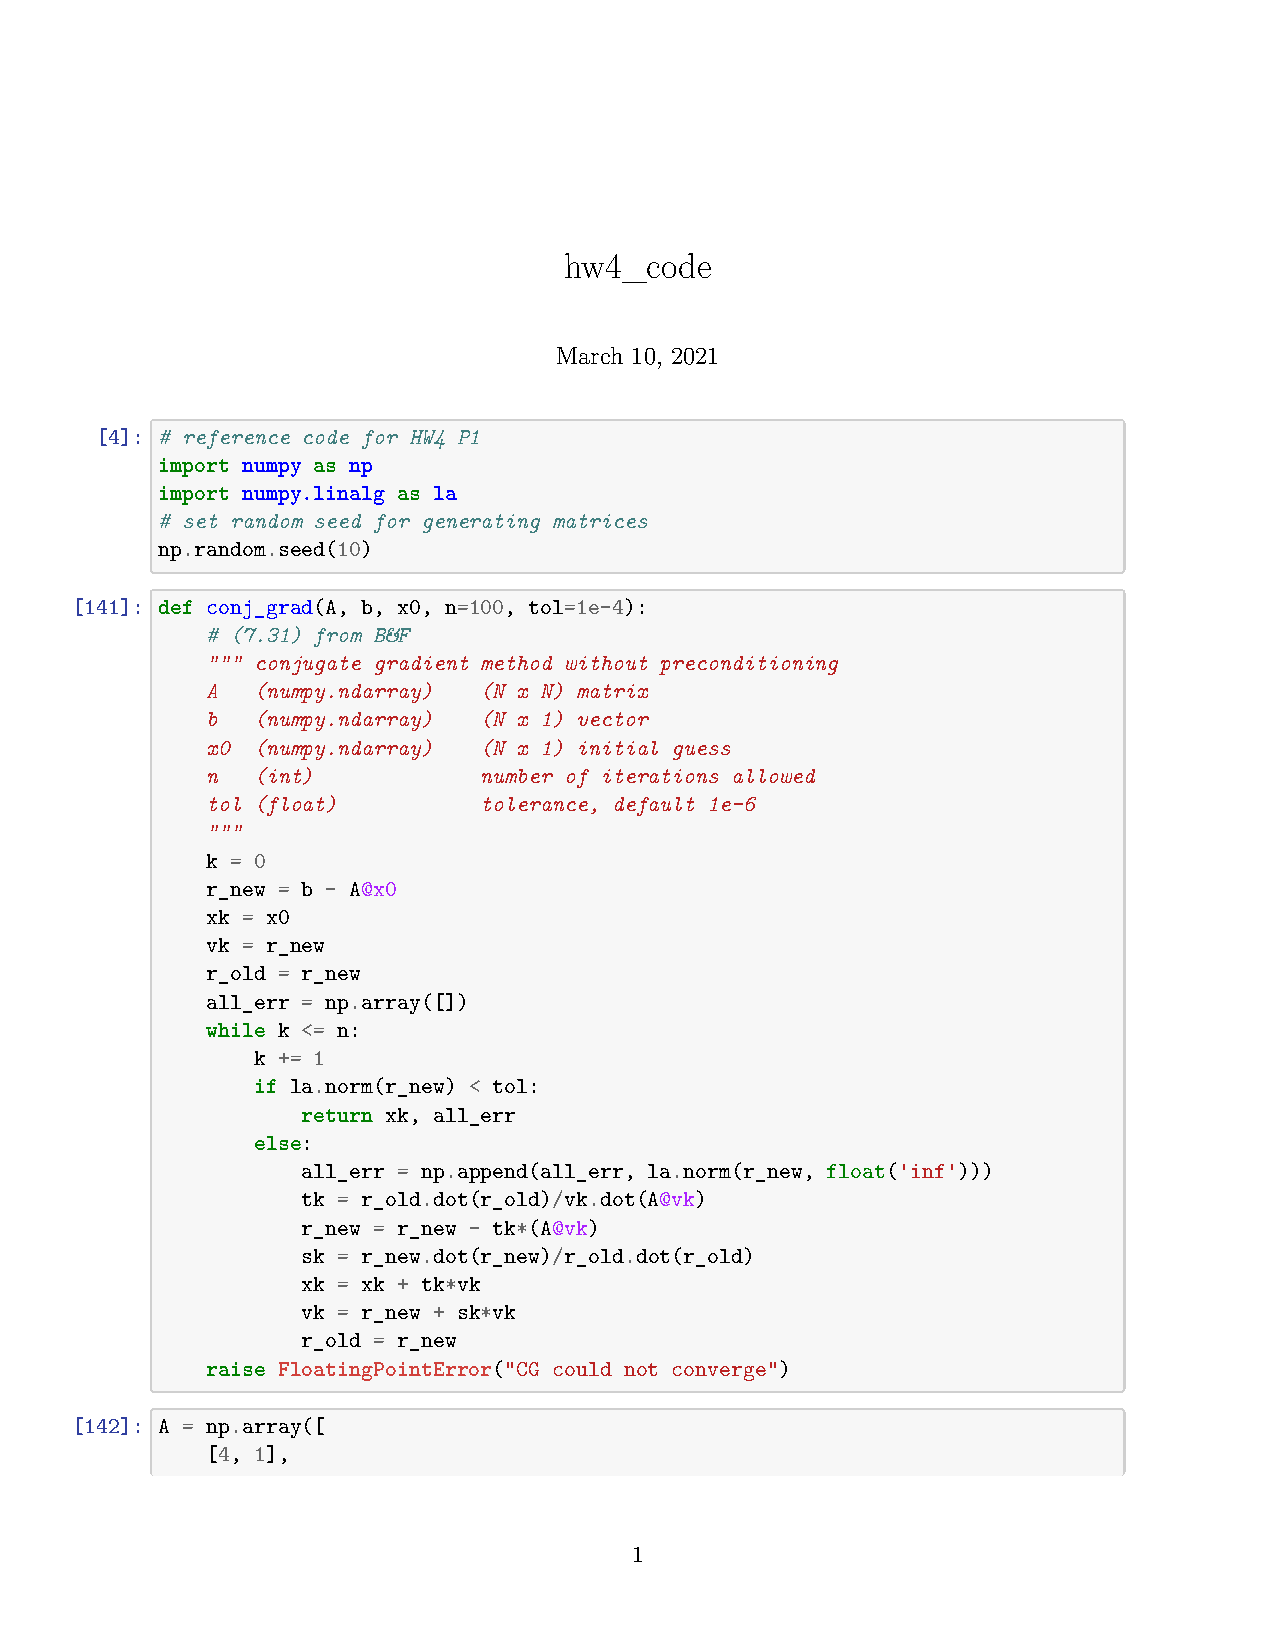
\includepdf[pages=-,scale=2,pagecommand={},width=\textwidth,linktodoc=true]{hw4_code.pdf}
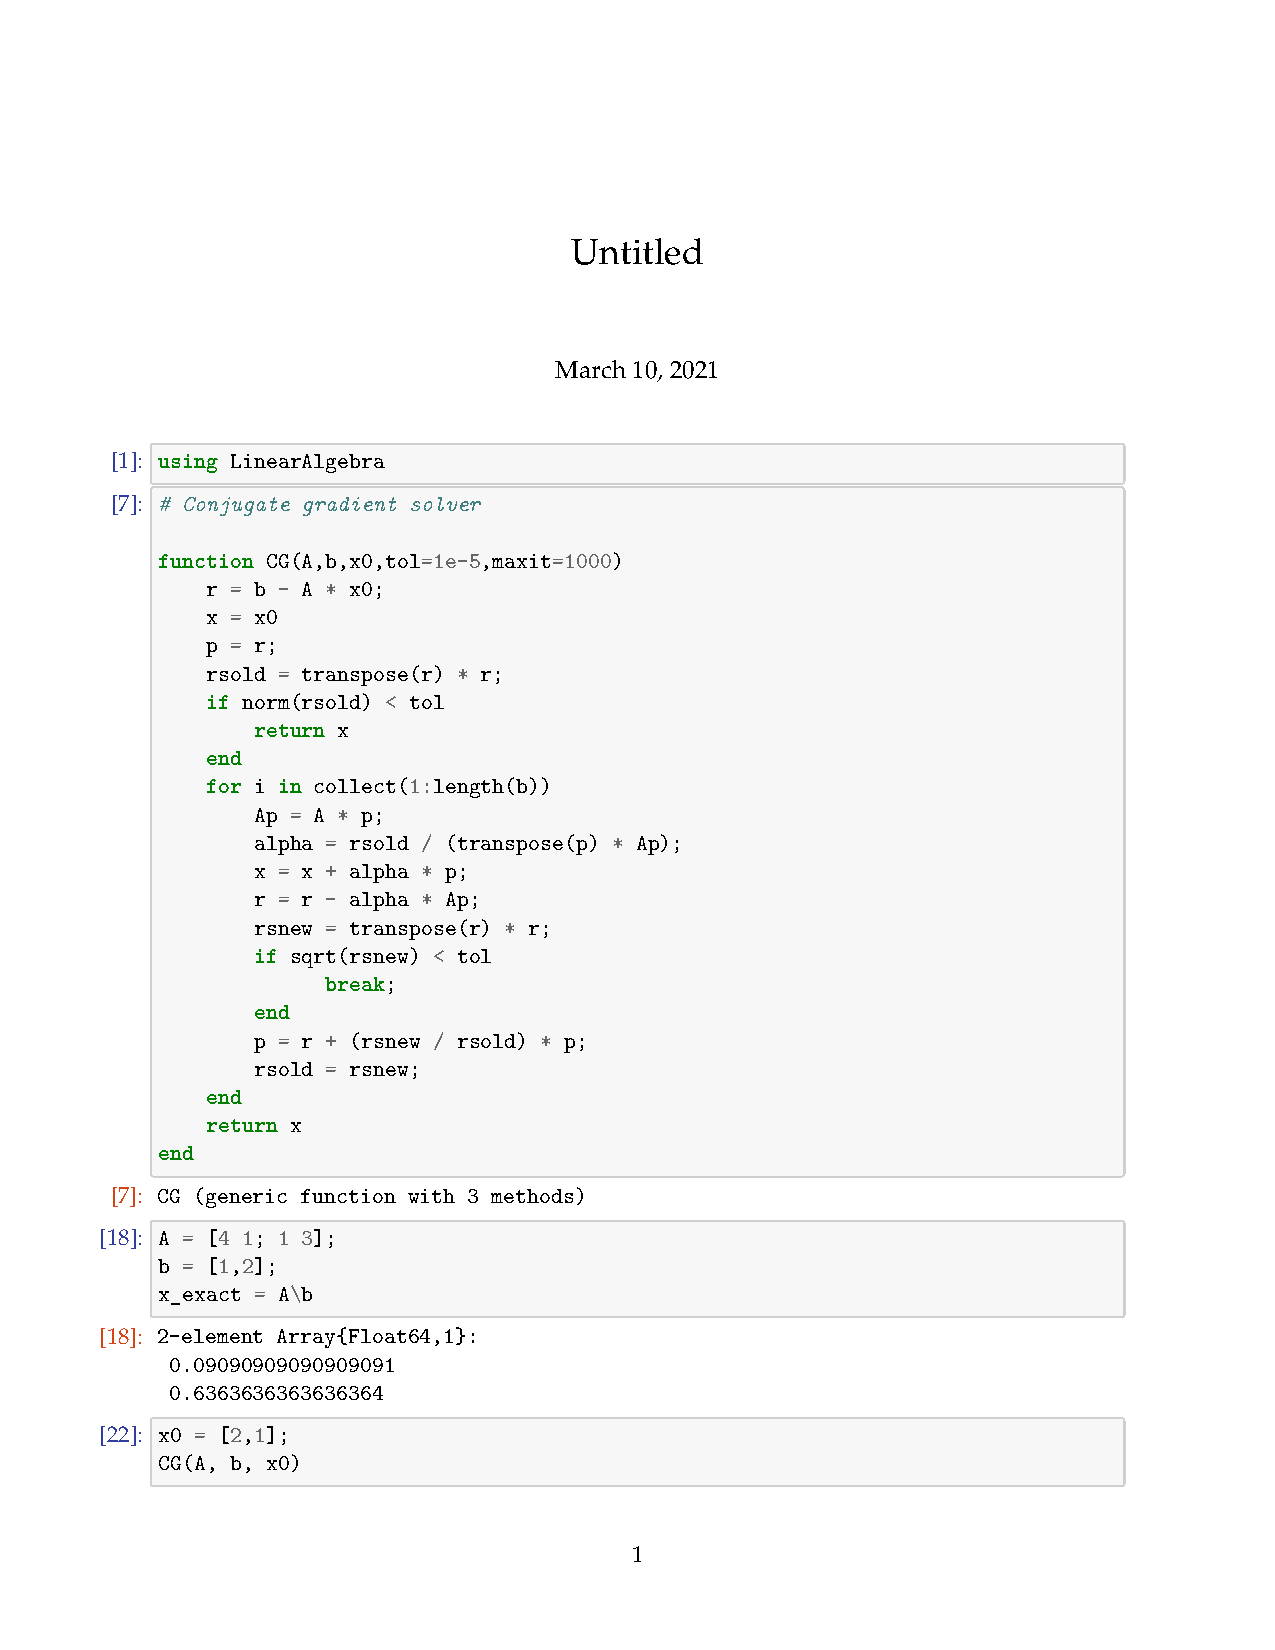
\includepdf[pages=-,scale=2,pagecommand={},width=\textwidth,linktodoc=true]{Untitled.pdf}

It is possible for CG to not converge if we set tolerance to be too low (close to machine $\eps$) or $\ka(A)$ is very large, which will cause numerical issues with floating point arithmetic (depending on specific choice of random matrices). Preconditioned CG is supposed to mitigate this issue. The correctness for this problem is graded based on correct implementation. 

\subsection{Rewrite CG with Preconditioning}
Rewrite CG algorithm in previous section with input matrix $C$. And discuss good and bad choices of $C$.
\subsubsection{}
Please refer to B\&F Algorithm 7.5 and convert it to MATLAB code. Correctness of this question is graded based on implementation. For the preconditioner, it is okay to try a few choices and discuss (good discussion involves trying a good preconditioner, a bad conditioner, and base solution $C=I$, and observe the effects of each on condition numbers and respective approximate solutions), the most common preconditioner is the incomplete Cholesky factorization (refer to B\&F last paragraph in section 7.6). The code should be at least correct when $C = I$, meaning there is no preconditioning at all.



\subsection{}
Use the Gershgorin Circle theorem to determine bounds for the eigenvalues and the spectral radius of the following matrices.

\subsubsection{a}
\emph{Errata}: The comments about eigenvalue locations are only empirically true. As predicted by the Theorem, the eigenvalues can be anywhere in the unioned circles. There are only upper bounds for the spectral radius $\rho(A)$. For more details, please post any questions / comments on Piazza post @50.




Follow Theorem 9.1, we first find the discs.
$$
A = \begin{pmatrix}
	4 & 0 & 1 & 3\\
	0 & 4 & 2 & 1\\
	1 & 2 & -2 & 0\\
	3 & 1 & 0 & 4
\end{pmatrix}
$$

Then respectively:
$$
R_1 = \{z\in \mathbb{C}: \abs{z-a_{11}} \le \sum_{j=1,j\neq 1}^{n}\abs{a_{1j}}\}
=
\{z\in \mathbb{C}: \abs{z-4} \le 4\}
$$
$$
	R_2 = \{z\in \mathbb{C}: \abs{z-a_{21}} \le \sum_{j=1,j\neq 2}^{n}\abs{a_{2j}}\}
=
\{z\in \mathbb{C}: \abs{z-4} \le 3\}
$$ we can see $R_2\subset R_1$.
$$
	R_3 = \{z\in \mathbb{C}: \abs{z-a_{31}} \le \sum_{j=3,j\neq 3}^{n}\abs{a_{3j}}\}
=
\{z\in \mathbb{C}: \abs{z+2} \le 3\}
$$
$$
	R_4 = \{z\in \mathbb{C}: \abs{z-a_{41}} \le \sum_{j=1,j\neq 4}^{n}\abs{a_{4j}}\}
=
\{z\in \mathbb{C}: \abs{z-4} \le 4\}
$$ therefore $R_2\subset R_1=R_4$. If we graph the discs on the complex plane, we see 2 circles centered at $z=4$ with radius 3 and 4, and 1 circle centered at $z=-2$ with radius 3. Furthermore, there are precisely 3 eigenvalues in $R_1$, and 1 eigenvalue in $R_3$.

Finally, 
$$
\rho(A) = \max_{i\in\{1,2,3,4\}}\abs{\lambda_i}
$$ and we can determine a bound:
$$
	\rho(A) \le 8
$$ by focusing on the region as far right on the real line as possible.





\subsubsection{b}
$$
A = \begin{pmatrix}
	1 & 0 & -1 & 1\\
	2 & 2 & -1 & 1\\
	0 & 1 & 3 & -2\\
	1 & 0 & 1 & 4
\end{pmatrix}
$$ similar to part (a), we determine:
$$
	R_1 = \{z\in \mathbb{C}: \abs{z-1} \le 2\}, R_2 = \{z\in \mathbb{C}: \abs{z-2} \le 4\}
$$
$$
	R_3 = \{z\in \mathbb{C}: \abs{z-3} \le 3\}, R_4 = \{z\in \mathbb{C}: \abs{z-4} \le 2\}
$$ 
$$
	\rho(A) \le 6
$$






\newpage
\subsection{Matrix Product Similarity}
Let $A,B$ be $n\times n$ and nonsingular, show that $AB$ is similar to $BA$.

\subsubsection{}
Refer to Definition 9.11 in B\&F, a matrix $M$ is said to be similar to $N$ if there is a nonsingular matrix $S$ such that:
$$
	M = S^{-1}NS
$$ similar matrices are important because the eigenvalues of $M$ are preserved through this transformation by $S$, which is a useful property in designing many iterative methods.

In this problem, we have $A, B$ both invertible. We can consider:
$$
	AB = A(BA)A^{-1}
$$ or:
$$
	BA = A^{-1}(AB)A
$$ then setting $M = BA$, $N = AB$, $S = A$ shows that $AB, BA$ are similar.
\newpage

% begin hw5
\section{Homework 5}
\subsection{Power Method}
Create a function which inputs matrix $A$, initial vector $x^{(0)}$, tolerance $tol$ and uses the power method with stopping criteria:
$$
	\norm{x^{(k)} - x^{(k-1)}}_{\infty} < tol	
$$ to obtain an approximate eigenpair $(\lambda, x)$. Test the algorithm on:
$$
	A = 
	\begin{pmatrix}
		2 & 1 & 1 \\
		1 & 2 & 1 \\
		1 & 1 & 2
	\end{pmatrix}, 
		x^{(0)} = 
		\begin{pmatrix}
		1\\
		-1\\
		2
		\end{pmatrix}, tol = 0.01
$$
\subsubsection{}
The matrix in our problem is symmetric, a Julia implementation of Algorithm 9.2 from textbook is as follows. If your eigenvector is not the same as displayed below, it is not incorrect as long as it is up to a scalar multiple of (the ones below).

\begin{figure}[t]
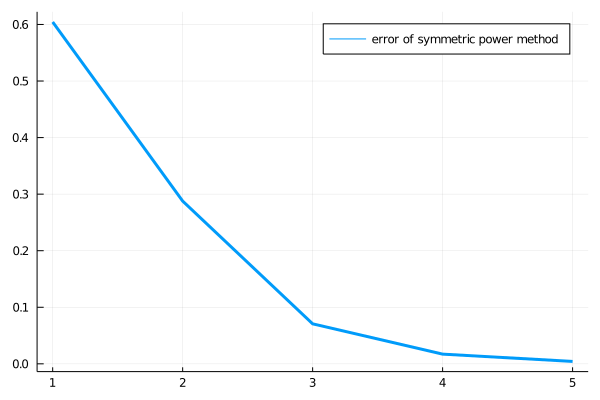
\includegraphics[width=12cm]{download.png}
\caption{Error of symmetric power method (Homework 5, Problem 1)}
\centering
\end{figure}


\subsection{}
Let:
$$
	A = 
	\begin{bmatrix}
		5 & 2 & 0 & 0\\
		1 & 4 & -1 & 0 \\
		0 & -1 & 4 & 2\\
		0 & 0 & 1 & 5
	\end{bmatrix}
$$ 

Use the Power Method, Wielandt deflation, and the Inverse Power method to approximate the eigenvalues and eigenvectors of $A$.

\textbf{\emph{Rubrics:}} This question is graded based on steps, procedures (if done on paper with the aid of linear solvers or calculators), or implementations (if done entirely in MATLAB). Two main points are update rules for approximate eigenvectors and that for eigenvectors. If student used MATLAB to perform Inverse Iteration with $q=0$, same credit was given if student did not implement Algorithm 9.3, and simply called the Power Method (implemented previously) with $A^{-1}$. Incomplete hand writing that does not show any steps how each vectors are obtained (namely only vectors with arbitrary numbers without context were written) calculations was penalized, despite final solutions are correct. For the Wielandt part, {\bf{points are not deducted}} if student does not use estimated dominant eigen-pairs, and had directly calculated true eigenvalues and eigenvectors, as solution has suggested.

Follow Algorithms 9.1, 9.3, 9.4 for MATLAB solution.

\subsubsection{}
$$
	A = \begin{pmatrix}
		5 & 2 & 0 & 0 \\
		1 & 4 & -1 & 0\\
		0 & -1 & 4 & 2\\
		0 & 0 & 1 & 5
	\end{pmatrix}
$$

If we solve the characteristic polynomials, we will find the following eigenvalues (sorted, exact calculations omitted).
$$
	\lambda_1 = 5+\sqrt{2} \approx 6.41421
$$
$$
	\lambda_2 = 4+\sqrt{3} \approx 5.73205
$$
$$
	\lambda_3 = 5-\sqrt{2} \approx 3.58579
$$
$$
	\lambda_4 = 4-\sqrt{3} \approx 2.26795
$$

With approximate eigenvectors (corresponding to the sorted eigenvalues):
$$
	v_1 \approx 
	\begin{pmatrix}
		-2.0 \\
		-1.414 \\
		1.414\\
		1.0
	\end{pmatrix}
$$
$$
	v_2 \approx 
	\begin{pmatrix}
		2.0 \\
		0.7321 \\
		0.7321\\
		1.0
	\end{pmatrix}
$$
$$
	v_3 \approx 
	\begin{pmatrix}
		-2.0 \\
		1.414 \\
		-1.414\\
		1.0
	\end{pmatrix}
$$
$$
	v_4 \approx 
	\begin{pmatrix}
		2.0 \\
		-2.7321 \\
		-2.7321\\
		1.0
	\end{pmatrix}
$$

Now we run the algorithms to approximate these values.
\subsubsection{Power Method}
We aim to use the Power iteration to find the largest eigenvalue and associated eigenvector $(\lambda_1, v_1)$. We use the steps outlined in chapter 9.3; since this algorithm is purely based on hitting the initial vector with $A$, it's okay to randomly pick an initial guess, so long as it is not 0. In here we choose:
$$
	x_0 = 
	\begin{pmatrix}
	1\\
	0\\
	0\\
	0
	\end{pmatrix}
$$

Hitting it with $A$ a few times gives us:
$$
	x_1 = Ax_0 = 
	\begin{pmatrix}
	5\\
	1\\
	0\\
	0
	\end{pmatrix},  
	x_2 = Ax_1 = 
	\begin{pmatrix}
	27\\
	9\\
	-1\\
	0
	\end{pmatrix}, 
	x_3 = Ax_2 = 
	\begin{pmatrix}
	153\\
	64\\
	-13\\
	-1
	\end{pmatrix}
$$
$$
	x_4 = Ax_3 = 
	\begin{pmatrix}
	893\\
	422\\
	-118\\
	-18
	\end{pmatrix},
	x_5 = Ax_4 = 
	\begin{pmatrix}
	5309 \\ 2699 \\
	-930 \\ -208
	\end{pmatrix},
	x_6 = Ax_5 = 
	\begin{pmatrix}
	31943\\17035\\-6835\\-1970
	\end{pmatrix}
$$

Then the sequence of eigenvalue approximations is:
$$
	\lambda_1^{(1)} = \frac{\norm{x_1}_{\infty}}{\norm{x_0}_{\infty}} = \frac{5}{1} = 5, 
	\lambda_1^{(2)} = \frac{\norm{x_2}_{\infty}}{\norm{x_1}_{\infty}} = \frac{27}{5} = 5.4
$$
$$
	\lambda_1^{(3)} = \frac{\norm{x_3}_{\infty}}{\norm{x_2}_{\infty}} = \frac{153}{27} \approx 5.6667, 
	\lambda_1^{(4)} = \frac{\norm{x_4}_{\infty}}{\norm{x_3}_{\infty}} = \frac{893}{153} \approx 5.8366
$$
$$
\lambda_1^{(5)} = \frac{\norm{x_5}_{\infty}}{\norm{x_4}_{\infty}} = \frac{5309}{893} \approx 5.94513, 
	\lambda_1^{(6)} = \frac{\norm{x_6}_{\infty}}{\norm{x_5}_{\infty}} = \frac{31943}{5309} \approx 6.0168
$$	

More steps are omitted, if we had some patience, we see:
$$
	x_{10}/\norm{x_{10}}_{\infty} \approx
	\begin{pmatrix}
	1.0\\  0.58898\\ -0.34148\\ -0.16187
	\end{pmatrix}, \lambda_1^{(10)}\approx 6.15682
$$
$$
	x_{20}/\norm{x_{20}}_{\infty} \approx 
	\begin{pmatrix}
	1.0\\  0.65843\\ -0.55397\\ -0.35731
	\end{pmatrix}, \lambda_1^{(20)}\approx 6.30707
$$

This approximates the largest eigenvalue to within $O(10^{-1})$, and it begins to converge very slowly (but it eventually will give us the eigenvalue). If we multiply the normalized vector $\widehat{x_{20}}$ by -2 to see whether we have a good approximation to $v_1$, we have:
$$
	\widehat{x_{20}}\cdot (-2) \approx 
	\begin{pmatrix}
	-2.0\\  -1.3169\\  1.1079\\  0.7146
	\end{pmatrix}
$$ which is not very good, but we are nearing the true values.
\subsubsection{Inverse Iteration}
If $A$ is invertible, applying the power method on $A^{-1}$ will yield the smallest eigenvalue and the corresponding eigenvector. This corresponds to setting $q=0$. If $A$ contains eigenvalues that are 0, this might not be a good idea; a remedy is to set $q$ to be a very small number so that $1/q <\infty$. 

In the following, we run the power method on $A^{-1}$. Take the starting value:
$$
	x^{(0)} = 
	\begin{pmatrix}
		1\\
		1\\
		1\\
		1
	\end{pmatrix}
$$ exact steps are similar to the previous part. Since only the eigenvalues are modified through $A^{-1}$, the eigenvectors should be the same as $A$. For an implementation, follow Algorithm 9.3 in textbook. Through some linear system solving, we have (after obtaining the scalars, invert them):
$$
\lambda_{4}^{(10)}\approx 2.27515, \lambda_{4}^{(20)}\approx 2.26802
$$ which yielded approximate eigenvectors (normalized):
$$
	v_4^{(10)} \approx 
	\begin{pmatrix}
		-0.73495\\  1.0\\ 0.98990 \\ -0.36029
	\end{pmatrix},
	v_4^{(20)} \approx
	\begin{pmatrix}
		-0.73208\\  1.0\\0.99990\\ -0.36597 
	\end{pmatrix}
$$ if we make the first entry $2$ by scaling, we see:
$$
	\widehat{v_4}^{(20)}\approx 
	\begin{pmatrix}
		2.0\\  -2.7319\\  -2.7316\\1.0
	\end{pmatrix}
$$ which is certainly very close to the true $v_4$.

\subsubsection{Wielandt Deflation}
The Wielandt Deflation fills in the rest of the eigenvalues, $\lambda_2, \lambda_3$. To be consistent with our calculations, we use the {\bf{estimated}} dominating eigen-pairs to feed into the deflation method. In realistic settings, we often do not know the exact dominating eigen-pairs. But through running Power Method for long enough, we will eventually get to one. 

The dominant eigen-pairs found through power method after 100 iterations:
$$
	\tilde{\lambda}_1 = \lambda_1^{(100)} \approx 
	6.41429
$$ with corresponding eigen-vector:
$$
	\tilde{v}_1= \tilde{v}_1^{(100)} \approx 
	\begin{pmatrix}
		-2.0\\ -1.4142764\\1.41441128\\1.00018424
	\end{pmatrix}
$$ these are close enough to the true solution. Let us use this eigenpair for the first deflation (need to normalize the eigenvector). The normalized vector is:
$$
	\widehat{\tilde{v}}_1 \approx
	\begin{pmatrix}-1.0\\ -0.707\\  0.707\\ 0.500\end{pmatrix} =: v_1
$$


The procedure is described in Theorem 9.20 of our textbook. Let $i=1$,
$$
	x = \frac{1}{\lambda_1(v_1)_1}(A_{11}, A_{12}, \cdots, A_{1n})^T = \frac{1}{6.41429\cdot (-1)}\cdot \begin{pmatrix}
	5\\
	2\\
	0\\
	0
	\end{pmatrix} \approx 
	\begin{pmatrix}
	-0.7795\\ -0.3118\\  0\\  0      
	\end{pmatrix}
$$

Then:
$$
	v_1\cdot x^T = \begin{pmatrix}
		-1.0\\ -0.707\\  0.707\\ 0.500
	\end{pmatrix}\cdot
	\begin{pmatrix}
	-0.7795 & -0.3118 &  0 &  0      
	\end{pmatrix}\approx
	\begin{pmatrix}
		0.7795 &  0.3118 &  0   &   0\\   
		0.5512&  0.2205&  0&   0\\
		-0.5513& -0.2205&  0 &  0\\
		-0.3898& -0.1559& 0 &  0    
	\end{pmatrix}
$$

Deflate matrix $A$:
$$
	B = A - \lambda_1 v_1\cdot x^T \approx
	\begin{pmatrix}
		O(10^{-6}) &  0&  0   &   0\\   
		-2.5357&  2.5857&  -1.0&   0\\
		3.536& 0.4144&  4.0 &  2.0\\
		2.5005& 1.0& 1.0 &  5.0   
	\end{pmatrix}
$$ then we can get rid of the first row and first column of $B$ to get a smaller matrix:
$$
	A' = 
	\begin{pmatrix}
	2.5857&  -1.0&   0\\
	0.4144&  4.0 &  2.0\\
	1.0& 1.0 &  5.0   
	\end{pmatrix}
$$

Now we can run Power Method again to find the second dominant eigen-pair. Exact steps are left out, after 100 iterations, we obtain:
$$
	\lambda_2^{(100)}\approx 5.7320
$$ with estimated (sub)-eigenvector (normalized):
$$
	w_2^{(100)}\approx\begin{pmatrix}
		-0.3178\\1.0\\0.9319
	\end{pmatrix}
$$ append a 0 entry, namely $w_2 = (0, -0.3178, 1.0, 0.9319)^T$, and we can recover via Equation (9.6) our $v_2$ approximation:
$$
	v_2  = (\lambda_2 - \lambda_1)w_2 + \lambda_1(x^Tw_2)v_1 \approx 
	\begin{pmatrix}
	2.0 \\
	0.731986404630087\\
	0.732253436240512\\
	1.00018881986252
	\end{pmatrix}
$$ as expected. The last eigenpair can be obtained in a similar way by deflating $B$ with the obtained pair $(\lambda_2, v_2)$.


\newpage
\subsection{}
Use Householder's method to place the following matrix in tridiagonal form:
$$
	A = 
	\begin{bmatrix}
		1 & 1 & 1 & 1 \\
		1 & 1 & 0 & 0 \\
		1 & 0 & 1 & 0 \\
		1 & 0 & 0 & 1
	\end{bmatrix}
$$
\subsubsection{}
Details for the concrete meaning of these numbers were outlined and developed in Lecture 11. Follow textbook Theorem 9.22. If you were following Page 606, there was a slight typo in $r$, where $\alpha_{k+1,k}$ should be $A_{k+1,k}$, the subdiagonal entry from the matrix.

To find $P^{(1)}$, we compute the following:
$$
	A^{(1)} = A = \begin{pmatrix}
		1 & 1 & 1 & 1 \\
		1 & 1 & 0 & 0 \\
		1 & 0 & 1 & 0 \\
		1 & 0 & 0 & 1
	\end{pmatrix}
$$
$$
	\alpha_1 = -sgn(A_{2,1}^{(1)})\sqrt{\bigg(
	\sum_{j=2}^{4}(A_{j1}^{(1)})^2
	\bigg)} = 
	-\sqrt{1^2 +1^2 + 1^2} = -\sqrt{3}
$$ 
$$
	r_1 = \sqrt{\frac{1}{2}\bigg(
	\alpha_1^2 - \alpha\cdot A_{2,1}^{(1)}
	\bigg)} = \sqrt{\frac12(3 +\sqrt{3}\cdot 1)} = \sqrt{\frac12(3+\sqrt{3})}
$$
$$
	w^{(1)} = 
	\begin{pmatrix}
		0 &
		\frac{A_{2,1}^{(1)} - \alpha_1}{2r_1}&
		\frac{A_{3,1}^{(1)}}{2r_1}&
		\frac{A_{4,1}^{(1)}}{2r_1}
	\end{pmatrix}^T = 
	(0, \frac{1+\sqrt{3}}{\sqrt{6+2\sqrt{3}}}, \frac{1}{\sqrt{6+2\sqrt{3}}}, \frac{1}{\sqrt{6+2\sqrt{3}}})^T
$$
$$
	P^{(1)} = I-2w^{(1)}(w^{(1)})^T = 
	\begin{pmatrix}
		1 & 0 & 0 & 0 \\
		0 & -\frac{2(1+\sqrt{3})^2}{6+2\sqrt{3}}+1 & -\frac{2(1+\sqrt{3})}{6+2\sqrt{3}} & -\frac{2(1+\sqrt{3})}{6+2\sqrt{3}}\\
		0 & -\frac{2(1+\sqrt{3})}{6+2\sqrt{3}} & 1-\frac{2}{6+2\sqrt{3}} & -\frac{2}{6+2\sqrt{3}}\\
		0 & -\frac{2(1+\sqrt{3})}{6+2\sqrt{3}} & -\frac{2}{6+2\sqrt{3}} & 1 - \frac{2}{6+2\sqrt{3}}
	\end{pmatrix}
$$ 

Then the first Householder transformation yields:
$$
	A^{(2)} = P^{(1)}\cdot A\cdot P^{(1)} = 
	\begin{pmatrix}
		1 & -\sqrt{3} & 0 & 0 \\
		-\sqrt{3} & 1 & 0 & 0 \\
		0 & 0 & 1 & 0 \\
		0 & 0 & 0 & 1
	\end{pmatrix}
$$ which is in tridiagonal form, therefore we stop.


\subsection{}
Modify Householder's algorithm to find a Hessenberg matrix similar to the matrix:
$$
	A = 
\begin{bmatrix}
		4 & 1 & 1 & 1 \\
		1 & 4 & 0 & 0 \\
		1 & 1 & 4 & 0 \\
		1 & 1 & 1 & 4
	\end{bmatrix}
$$
\subsubsection{}
Would like to run Householder to reduce:
$$
A = 
\begin{pmatrix}
		4 & 1 & 1 & 1 \\
		1 & 4 & 0 & 0 \\
		1 & 1 & 4 & 0 \\
		1 & 1 & 1 & 4
	\end{pmatrix}
$$ to upper Hessenberg form. Following Algorithm 9.5 plus the modifications.
$$
	k = 1, A^{(1)} = A
$$ 
$$
	q_1 = \sum_{j=2}^4 (A_{j1})^2 = 1^2 + 1^2 + 1^2 = 3
$$
$$
	\alpha_1 = -\frac{\sqrt{q_1}\cdot A_{21}}{\abs{A_{21}}} = -\sqrt{3}
$$
$$
	2r_1^2 = RSQ = \alpha_1^2 - \alpha_1\cdot A_{21} = 3+\sqrt{3}
$$
$$
	v_1 = 0, v_2 = A_{21}-\alpha_1 = 1+\sqrt{3}, v_3 = A_{31} = 1, v_4 = A_{41} = 1
$$ (Step 6 is modified as the following):
$$
	u_1 = \frac{1}{RSQ}\sum_{i=2}^4A_{1i}v_i = \frac{1}{3+\sqrt{3}}(1\cdot (1+\sqrt{3}) + 1\cdot 1 + 1\cdot 1) = 1
$$
$$
	u_2 = \frac{1}{RSQ}\sum_{i=2}^4A_{2i}v_i = \frac{4\cdot (1+\sqrt{3})}{3+\sqrt{3}} = \frac{4+4\sqrt{3}}{3+\sqrt{3}}
$$
$$
u_3 = \frac{1}{RSQ}\sum_{i=2}^4A_{3i}v_i = \frac{1+\sqrt{3} + 4\cdot 1}{3+\sqrt{3}} = \frac{5+\sqrt{3}}{3+\sqrt{3}}
$$
$$
u_4 = \frac{1}{RSQ}\sum_{i=2}^4A_{4i}v_i = \frac{(1+\sqrt{3} + 1 + 4)}{3+\sqrt{3}} = \frac{6+\sqrt{3}}{3+\sqrt{3}}
$$
$$
	y_1 = \frac{1}{RSQ}\sum_{i=2}^4 A_{i1}v_i = \frac{1+\sqrt{3}+1+1}{3+\sqrt{3}} = 1
$$
$$
	y_2 = \frac{1}{RSQ}\sum_{i=2}^4 A_{i2}v_i =\frac{4\cdot (1+\sqrt{3}) + 1+1}{3+\sqrt{3}} = \frac{6+4\sqrt{3}}{3+\sqrt{3}}
$$
$$
y_3 = \frac{1}{RSQ}\sum_{i=2}^4 A_{i3}v_i = \frac{4+1}{3+\sqrt{3}} = \frac{5}{3+\sqrt{3}}
$$
$$
y_4 = \frac{1}{RSQ}\sum_{i=2}^4 A_{i4}v_i = \frac{}{3+\sqrt{3}} = \frac{4}{3+\sqrt{3}}
$$ Now step 7:
$$
	PROD = \sum_{j=2}^4 v_ju_j = \frac{(1+\sqrt{3})(4+4\sqrt{3})}{3+\sqrt{3}} + \frac{5+\sqrt{3}}{3+\sqrt{3}} + \frac{6+\sqrt{3}}{3+\sqrt{3}} = \frac{\sqrt{3}+17}{2}
$$ step 8:
$$
	z_1 = u_1 - \frac{PROD}{RSQ}v_1 = 1
$$
$$
	z_2 = u_2 - \frac{PROD}{RSQ}v_2 = -\frac{1+3\sqrt{3}}{2}
$$
$$
	z_3 = u_3 - \frac{PROD}{RSQ}v_3 = -2+\frac{5}{6}\sqrt{3}
$$
$$
z_4 = u_4 - \frac{PROD}{RSQ}v_4 = -3+\frac{7}{6}\sqrt{3}
$$ step 9:
$$
	A^{(2)}_{12} =A_{12} - z_1v_2 = 1-1-\sqrt{3} = -\sqrt{3}
$$
$$
	A_{21}^{(2)} = A_{21}-y_1v_2=1-1-\sqrt{3} = -\sqrt{3}
$$
$$
A_{22}^{(2)} = A_{22}-z_2v_2-y_2v_2 = 4+\frac{(1+3\sqrt{3})(1+\sqrt{3})}{2} - \frac{(6+3\sqrt{3})(1+\sqrt{3})}{3+\sqrt{3}}=5
$$	
$$
	A_{32}^{(2)} = A_{32} - z_3v_2 - y_2z_3 = 1-(-2+\frac{5}{6}\sqrt{3})(1+\sqrt{3}) - \frac{6+4\sqrt{3}}{3+\sqrt{3}} \approx -0.2113
$$
$$
	A_{42}^{(2)}=A_{42} - z_4v_2 - y_2v_4 =1-(-3+\frac{7}{6}\sqrt{3})(1+\sqrt{3}) - \frac{6+4\sqrt{3}}{3+\sqrt{3}}\approx 0.9434
$$
$$
	A_{13}^{(2)} = A_{13} - z_1v_3 = 1-1=0
$$
$$
	A_{31}^{(2)} = A_{31} - y_1v_3 = 1-1=0
$$
$$
	A_{23}^{(2)} = A_{23} - z_2v_3 - y_3v_2 = 0+\frac{(1+3\sqrt{3})}{2}-\frac{5(1+\sqrt{3})}{3+\sqrt{3}} \approx 0.2113
$$
$$
	A_{33}^{(2)} = A_{33} - z_3v_3 - y_3v_3 = 4-(-2+\frac56\sqrt{3}) - \frac{5}{3+\sqrt{3}} \approx 3.5
$$
$$
	A_{43}^{(2)} = A_{43} - z_4v_3 - y_3v_4 = 1-(-3+\frac76\sqrt{3}) - \frac{5}{3+\sqrt{3}} \approx 0.9226
$$
$$
	A_{14}^{(2)} = A_{14} - z_1v_4 = 1-1=0
$$
$$
	A_{41}^{(2)} = A_{41} - y_1v_4 = 1-1=0
$$
$$
	A_{24}^{(2)} = A_{24} - z_2v_4 - y_4v_2 = \frac{1+3\sqrt{3}}{2} - \frac{4(1+\sqrt{3})}{3+\sqrt{3}} = \approx 0.7887
$$
$$
	A_{34}^{(2)} = A_{34} - z_3v_4 - y_4v_3 = 2-\frac56\sqrt{3} - \frac{4}{3+\sqrt{3}}\approx -0.2887
$$
$$
	A_{44}^{(2)} = A_{44} - z_4v_4 - y_4v_4 = 3.50
$$

One step of Householder transformation should yield:
$$
	A^{(2)} = 
	\begin{pmatrix}
		4 & -\sqrt{3} & 0 & 0 \\
		-\sqrt{3} & 5 & 0.2113 & 0.7887 \\
		0 & -0.2113 & 3.50 & -0.2887 \\
		0 & 0.9434& 0.9226 & 3.50
	\end{pmatrix}
$$


Another step should yield the end result, close to:
$$
	\begin{pmatrix}
		4&   -1.732&   0&   0\\
		-1.732 & 5 & -0.817 & 0\\
		0 & 0.817 & 3.50 & 0.289\\
		0 & 0 & -0.289 & 3.50
	\end{pmatrix}
$$

% begin midterm
\newpage
\section{Midterm Exam}
\subsection{Limit of Matrix Power}
Determine, with proof the limit:
$$
	\ntoinf{n}A^nv
$$ where:
$$
	A = 
	\begin{pmatrix}
		2/3 & -3 & 12\\
		0 & 1/2 & 1/2\\
		0 & 1/3 & 1/2
	\end{pmatrix}, 
	v = 
	\begin{pmatrix}
		1 \\
		-1\\
		1
	\end{pmatrix}
$$



\subsubsection{}
$$
A = 
\begin{pmatrix}
	\frac23& -3& 12\\
    0& \frac12& \frac12\\
    0& \frac13& \frac12
\end{pmatrix}
$$ 

It is enough to show that $A$ is a convergent matrix, we do so by computing eigenvalues by hand:
$$
	A - \lambda I = 
	\begin{pmatrix}
	\frac23-\lambda& -3& 12\\
    0& \frac12-\lambda& \frac12\\
    0& \frac13& \frac12-\lambda
\end{pmatrix}
$$ then set:
$$
	\det(A-\lambda I) = 0
$$ and solve:
$$
(\frac23-\lambda)\bigg[
(\lambda-\frac12)^2 - \frac16
\bigg] = 0
$$ after some computations, we conclude the our eigenvalues are:
$$
	\lambda_1 = \frac23, \lambda_2 = \frac{1}{2}+\frac{1}{\sqrt{6}}, \lambda_3 = \frac{1}{2}-\frac{1}{\sqrt{6}}
$$

Since electronics were prohibited, let's bound $\frac{1}{\sqrt{6}}$, we have $\frac{1}{\sqrt{6}} < \frac12$ since $\sqrt{6} > 2$ then we have:
$$
\frac12 + \frac{1}{\sqrt{6}} < 1/2 + 1/2 = 1
$$ and certainly:
$$
	0<\frac12 - \frac{1}{\sqrt{6}}<1
$$

In short, $\rho(A) < 1$: we have by Theorem 7.17 of BF that $A$ is convergent, as a consequence:
$$
	\ntoinf{n}A^nv = 0
$$


\subsection{${l}_2$-norm and condition number}
Determine, with proof, the $l_2$-norm and 2-condition number of the matrix:
$$
	A=
	\begin{pmatrix}
		2 & 1\\
		1 & 0
	\end{pmatrix}
$$

\subsubsection{}
First $l_2$ norm:
$$
	\norm{A}_2^2 = \lambda_{max}(A^TA)
$$ the largest eigenvalue of $A^TA$. We have:
$$
	B = A^TA = 
	\begin{pmatrix}
		5 & 2 \\
		2 & 1
	\end{pmatrix}
$$ and compute:
$$
	\det(B - \lambda I) = (\lambda-5)(\lambda-1)-4=0
$$ and solve, we have:
$$
\lambda = 3\pm 2\sqrt{2}
$$ then the largest eigenvalue is $\lambda = 3+2\sqrt{2}$. Then:
$$
	\norm{A}_2 = \sqrt{3+2\sqrt{2}}
$$

The condition number is the two norm sense is:
$$
	\ka(A) = \norm{A}_2\cdot\norm{A^{-1}}_{2}
$$

$A$ is a nice symmetric matrix, we can write its eigendecomposition as:
$$
	A = PDP^{-1}
$$ where $P$ is orthogonal. Then we have:
$$
	A^{-1} = PD^{-1}P^{-1}
$$ therefore nothing changed except for inverse eigenvalues.

We have:
$$
	\norm{A^{-1}}_2^2 = \lambda_{\max}(A^{-T}A^{-1}) = \lambda_{\max}((AA^T)^{-1})
$$

We have:
$$
	AA^T = A^TA= 
	\begin{pmatrix}
		5 & 2 \\
		2 & 1
	\end{pmatrix}
$$ whose inverse is:
$$
	(AA^T)^{-1} = 
	\begin{pmatrix}
		1 & -2 \\
		-2 & 5
	\end{pmatrix}
$$ since this is a 2 by 2 matrix, in Math 54 or Math 110 we might have seen a handy trick to compute an inverse quickly (swap $a, d$ and swap $b, c$ then negate), and the determinant of $AA^T$ happens to be 1. 

We now find the eigenvalues of this new matrix by computing:
$$
	\det(B^{-1}-\lambda I) = 0
$$ and solve:
$$
	(\lambda -5)(\lambda -1) = 4
$$ which is the same as before, then we can conclude:
$$
	\ka(A) = \norm{A}_2\cdot\norm{A^{-1}}_2 = 3+2\sqrt{2}
$$














\newpage
\subsection{Jacobi Method Computations}
Let initial vector be $x^{(0)} = 0$, find two iterations of the Jacobi Method for the following linear system:
$$
	-2x_1 + x_2 + \frac12x_3 = 4
$$
$$
	x_1 - 2x_2 - \frac12x_3 = 2
$$
$$
	x_2 + 2x_3 = 0
$$
\subsubsection{}
\emph{Note}: In class and also in BF, we defined the strictly lower, strictly upper, triangular part to be $-L, -U$.

In this problem we have:
$$
	A = 
	\begin{pmatrix}
		-2 & 1 & \frac12 \\
		1 & -2 & -\frac12 \\
		0 & 1 & 2
	\end{pmatrix},
	b = 
	\begin{pmatrix}
		4\\
		2\\
		0 
	\end{pmatrix}
$$ with initial vector $x^{(0)} = 0$.

By (7.6) in BF, the Jacobi Matrix Update Rule is:
$$
	x^{(i+1)} = D^{-1}(L+U)x^{(i)} + D^{-1}b
$$ where $D+L+U=A$ are diagonal, lower triangular part, upper triangular part. There is no complicated inverse, and:
$$
	D^{-1} = 
	diag([-\frac12, -\frac12, \frac12])
$$

And:
$$
	c = D^{-1}b = 
	\begin{pmatrix}
		-1/2 & 0 & 0 \\
		0 & -1/2 & 0 \\
		0 & 0 & 1/2
	\end{pmatrix}
	\begin{pmatrix}
		4\\
		2\\
		0 
	\end{pmatrix} = 
	\begin{pmatrix}
		-2\\
		-1\\
		0 
	\end{pmatrix}
$$

$$
	T = 
	-D^{-1}(L+U) = 
	-\begin{pmatrix}
		-1/2 & 0 & 0 \\
		0 & -1/2 & 0 \\
		0 & 0 & 1/2
	\end{pmatrix}
	\Bigg[
	\begin{pmatrix}
		0 & 0 & 0 \\
		1 & 0 & 0 \\
		0 & 1 & 0
	\end{pmatrix}+
	\begin{pmatrix}
		0 & 1 & 1/2 \\
		0 & 0 & -1/2 \\
		0 & 0 & 0
	\end{pmatrix}
	\Bigg]
$$
$$
	T = \begin{pmatrix}
		0&1/2  & 1/4 \\
		1/2&0 & -1/4 \\
		0 & -1/2 &0
	\end{pmatrix}
$$

Using $T$ and $c$, two iterations are:
$$
	x^{(1)} = 
	\begin{pmatrix}
		-2\\
		-1\\
		0 
	\end{pmatrix}
$$
$$
	x^{(2)} = 
	\begin{pmatrix}
		-5/2\\
		-2\\
		1/2 
	\end{pmatrix}
$$

\subsection{Householder Matrix Eigenvalues}
Find eigenvalues of a real $n\times n$ Householder matrix $I - ww^T$ where $\norm{w}_2 = 1$.
\subsubsection{}
The householder matrix:
$$
	H = I - 2ww^{T}
$$ where we have $\norm{w}_2 =\sqrt{w^Tw} =1$. Here $w$ is a column vector, $ww^T$ means vector outer product with itself, and is a matrix. It doesn't make much sense to talk about $I - 2w^Tw$.

$ww^T$ has a nice property that it is symmetric, and $I-2ww^T$ will be symmetric as well. The eigenvalues of real symmetric matrices are real. In matrix notation, we can see:
$$
	(I-2ww^T)^T = I^T - 2(ww^T)^T = I - 2ww^T
$$ and also since $w$ is a unit vector, $H$ is orthogonal:
$$
	(I-2ww^T)(I-2ww^T) = I-4ww^T+4ww^Tww^T
$$
$$
	= I-4ww^T+4w(w^Tw)w^T = I
$$

In Math 110 we may have proved in one of the homework assignments that orthogonal matrices only have eigenvalues with magnitude 1. But $H$ is symmetric, thus all eigenvalues of $H$ are real. Then we know that the only possible eigenvalues of $H$ here are $\pm 1$ (should be proved). Indeed:
$$
	(I - 2ww^T)w = w - 2w(w^Tw) = w-2w = -w = (-1)\cdot w
$$ and take any unit vector $v$ such that $w\perp v$, we have:
$$
	(I - 2ww^T)v = Iv - 2ww^Tv = Iv = v = (1)\cdot v
$$

\newpage
% begin HW 6
\section{Homework 6}
\subsection{QR Decomposition}
Create a function that implements the QR decomposition with shifts. Use the algorithm to determine, within $10^{-5}$ all eigenvalues of the matrix:
$$
	A=
	\begin{pmatrix}
		2 & -1 & 0 \\
		-1 & -1 & 2 \\
		0 & -2 & 3
	\end{pmatrix}
$$
\subsubsection{}
A Julia implementation is attached below for reference (Following Algorithm 9.6 in book). The eigenvalues should be close to:
$$
	\lambda_1 \approx 3.912, \lambda_2 \approx 2.130, \lambda_3 \approx -2.041
$$

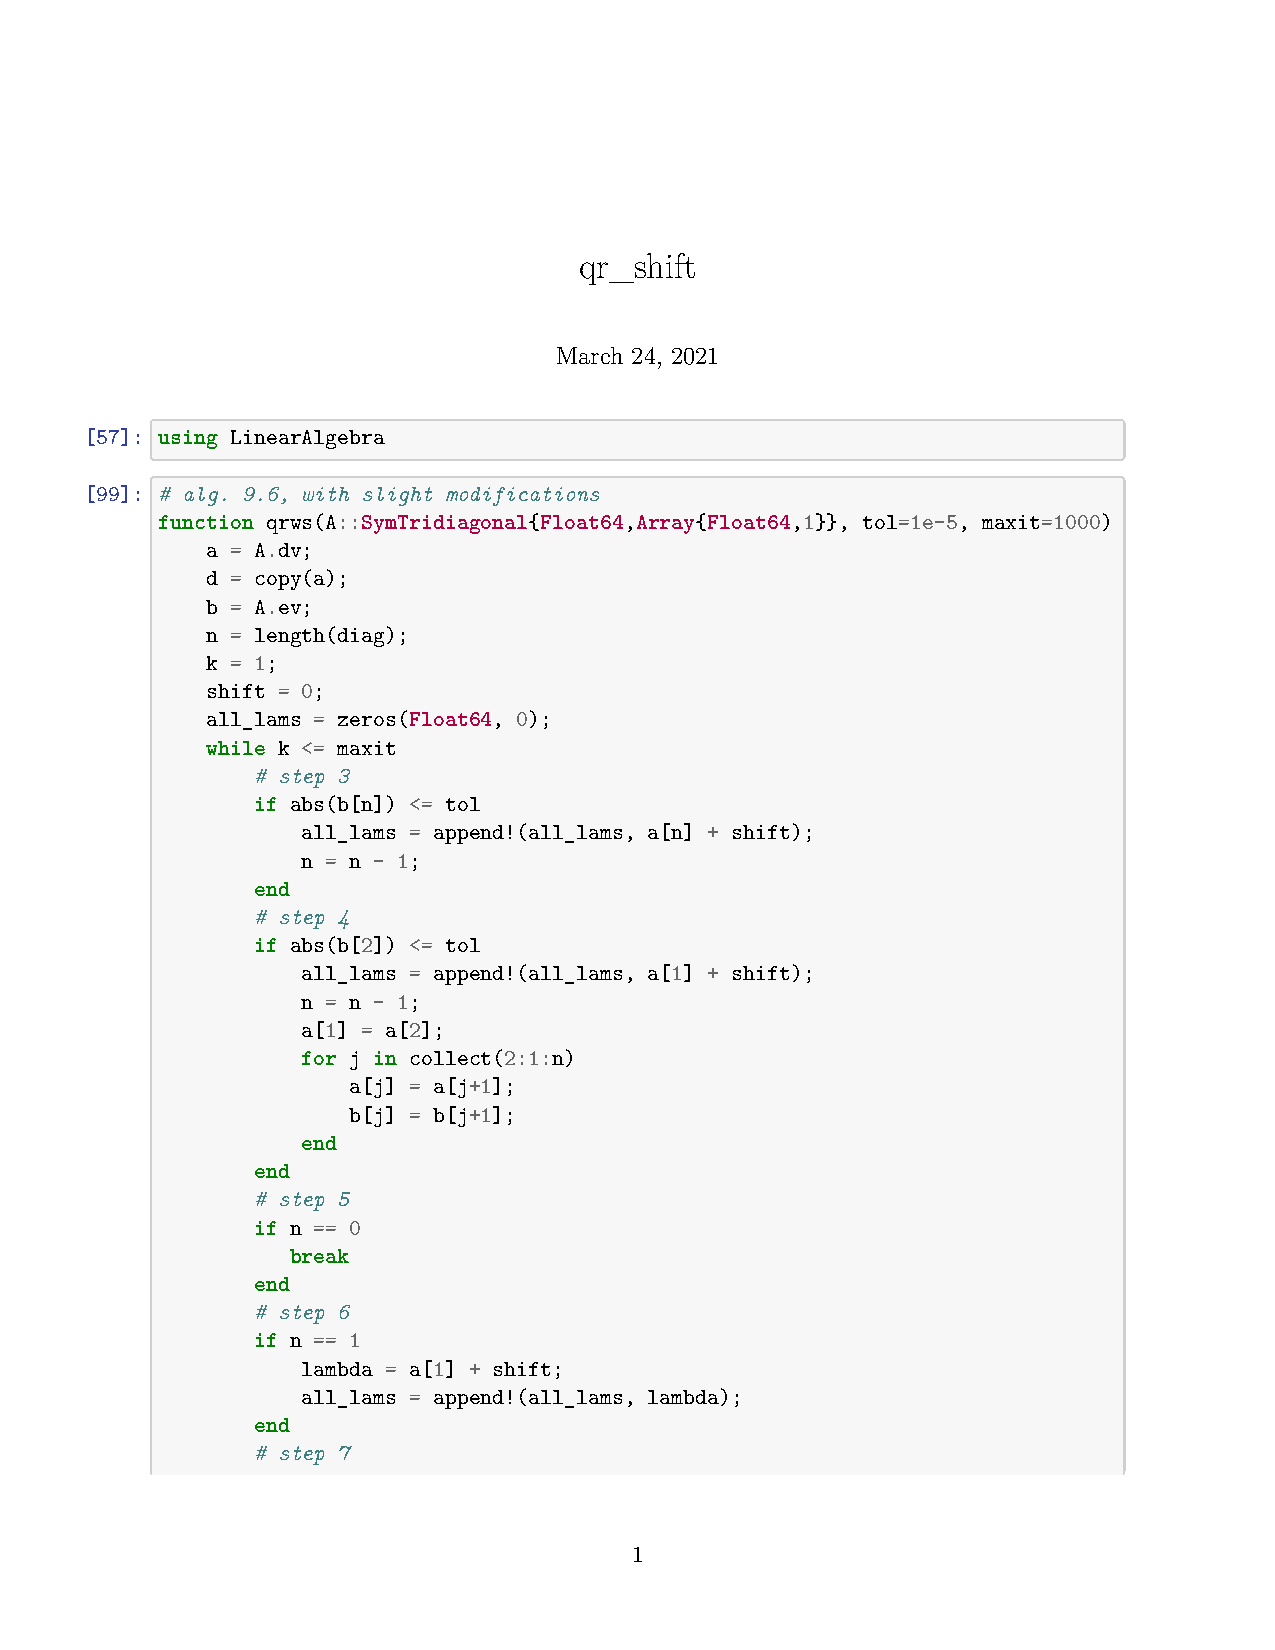
\includepdf[pages=-,scale=2,pagecommand={},width=\textwidth,linktodoc=true]{qr_shift.pdf}





\newpage
\subsection{Find Singular Values}
Determine singular values of the following matrices:
$$
\begin{pmatrix}
	2 & 1 \\
	1 & 1 \\
	0 & 1
\end{pmatrix}, 
\begin{pmatrix}
	1 & 1 & 0 \\
	1 & 0 & 1 \\
	0 & 1 & 1
\end{pmatrix}
$$	


\subsubsection{a}
We can compute the singular values by hand using Definition 9.27.

$$
	A = 
	\begin{pmatrix}
		2 & 1 \\
		1 & 1\\
		0 & 1
	\end{pmatrix}
$$
$$
	B = A^TA = 
	\begin{pmatrix}
		5 & 3 \\
		3 & 3
	\end{pmatrix}
$$ then we solve $\det(B - \lambda I) = 0$, or:
$$
	\det\bigg[\begin{pmatrix}
		5-\lambda & 3 \\
		3 & 3-\lambda
	\end{pmatrix}\bigg] = \lambda^2 - 8\lambda - 6 = 0
$$
$$
	\lambda_1 = 4+\sqrt{10}, \lambda_2 = 4-\sqrt{10}
$$

Then the two singular values are:
$$
	\sigma_1 = \sqrt{4+\sqrt{10}}, \sigma_2 = \sqrt{4-\sqrt{10}}
$$


\subsubsection{b}
$$
	A = 
	\begin{pmatrix}
		1 & 1 & 0\\
		1 & 0 & 1\\
		0 & 1 & 1
	\end{pmatrix}
$$

Then:
$$
	B = A^TA = 
	\begin{pmatrix}
		2 & 1 & 1\\
		1 & 2 & 1\\
		1 & 1 & 2
	\end{pmatrix}
$$ then solve $\det(B-\lambda I) = 0$, or:
$$
	-(\lambda-2)^3 + 3\lambda - 4 = 0
$$ then:
$$
	\lambda_1 = 4, \lambda_2=\lambda_3 = 1
$$

$A$ has full rank, then we have 3 singular values:
$$
	\sig_1 = 2, \sig_2=\sig_3 = 1
$$


\subsection{$l_2$-condition number}
Show that if $A$ is a matrix with singular values $s_1,s_2,\cdots, s_n$, then its $l_2$-condition number is equal to:
$$
	\ka(A) = \frac{s_1}{s_n}
$$
\subsubsection{}
By definition of two norm condition number:
$$
	\ka(A) = \norm{A}_2\norm{A^{-1}}
$$ where $A$ is nonsingular and admits the SVD:
$$
	A = U\Sigma V^*
$$ where $U,V$ are both unitary. 

\subsubsection{preservation of norm by unitary matrix}
Let $U$ be unitary, $x$ be a vector, then:
$$
	\norm{Ux}_2^2 = x^*U^*Ux = x^*x = \norm{x}_2^2
$$ therefore norm is preserved by unitary transformations.


\subsubsection{two norm of $A$}
$$
	\norm{A}_2 = \sup_{\norm{x}_2 = 1}\norm{Ax}_2 = \sup_{\norm{x}=1}\norm{U\Sigma V^*x}_2 = \sup_{\norm{x}=1}\norm{\Sigma V^*x}_2 = \sup_{\norm{x}=1}\norm{\Sigma y}_2
$$ renaming $y = V^*x$.
$$
	= \sup_{\norm{x}=1}\bigg( 
	\sum_{1}^n s_i^2\abs{y_i}^2
	\bigg)^{1/2} = 
	\sup_{\norm{y}=1}\bigg( 
	\sum_{1}^n s_i^2\abs{y_i}^2
	\bigg)^{1/2} = s_1
$$ where the last equality comes from $\norm{x} = \norm{V^*x} = \norm{y}$. (WLOG assume the singular values are sorted) The maximum is attainable at $y = (1, 0, \cdots, 0)$.

\subsubsection{two norm of $A^{-1}$}
$A$ is invertible by assumption, then:
$$
	A^{-1} = (U\Sigma V^*)^{-1} = V\Sigma^{-1}U^*
$$ where $\Sigma^{-1}$ is the diagonal matrix containing the inverse of the singular values of $\Sigma$. Then by a similar argument as before, we conclude:
$$
	\norm{A^{-1}}_2 = 1/s_n 
$$ because $s_n < s_{n-1} < \cdots < s_1$.


\subsubsection{conclusion}
As above, we conclude:
$$
	\ka(A) = \norm{A}_2\norm{A^{-1}}_2 = s_1/s_n
$$ as desired.


\newpage
% begin HW 7
\section{Homework 7}
\subsection{Least Squares Polynomial Approximation}
Find the least squares approximation of degree 2 and 3 to:
$$
	f(x) = e^x
$$ on the interval $[-1,1]$.
\subsubsection{}
$$
	f(x) = e^x
$$ we would like to find respectively degree 2 and 3 least squares polynomial approximation on $[-1,1]$. The goal of least squares is to minimize:
$$
	\int_{-1}^1 (f(x) - P_n(x))^2dx
$$ where:
$$
	P_2(x) =a_2x^2 + a_1x+a_0
$$
$$
	P_3(x) = a_3x^3 + a_2x^2 + a_1x + a_0
$$ using (8.6) from textbook, we need to solve the normal equations for $j = 0,1,\cdots, n$:
$$
	\sum_{k=0}^2a_k\int_{-1}^{1}x^{j+k}dx = \int_{-1}^1x^jf(x)dx
$$

For $n=2$, we have the following:
$$
\begin{cases}
		a_0\int_{-1}^1 1dx +a_1\int_{-1}^1xdx + a_2\int_{-1}^1x^2dx= \int_{-1}^1e^xdx\\
		a_0\int_{-1}^1 xdx +a_1\int_{-1}^1x^2dx + a_2\int_{-1}^1x^3dx= \int_{-1}^1xe^xdx\\
		a_0\int_{-1}^1 x^2dx +a_1\int_{-1}^1x^3dx + a_2\int_{-1}^1x^4dx= \int_{-1}^1x^2e^xdx
\end{cases}
$$ which yields the following linear system:
$$
	\begin{pmatrix}
	2 & 0 & 2/3 \\
	0 & 2/3 & 0\\
	2/3 & 0 & 2/5
	\end{pmatrix}
	\begin{pmatrix}
	a_0\\
	a_1\\
	a_2
	\end{pmatrix}=
	\begin{pmatrix}
	e-\frac1e\\
	\frac2e\\
	e-\frac5e
	\end{pmatrix}
$$

Using a linear solver, we obtain:
$$
	a \approx \begin{pmatrix}0.53672153\\ 1.10363832\\ 0.99629402\end{pmatrix}
$$

The following plots show a degree-2 approximation would yield a degree-3 residual, as expected.
\begin{figure}[h]
\centering
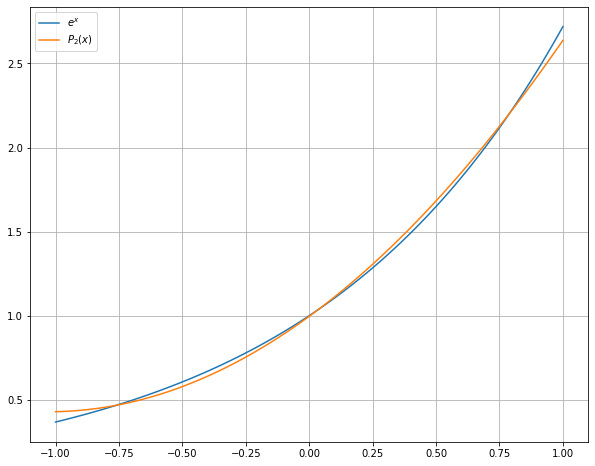
\includegraphics[width=0.8\textwidth]{p1poly2.png}
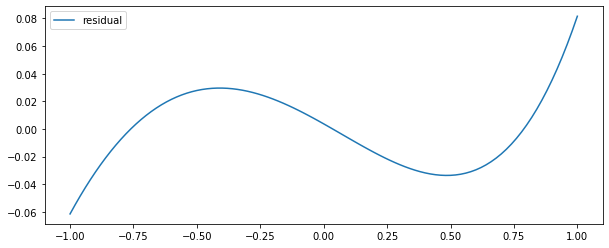
\includegraphics[width=0.8\textwidth]{p1poly2_res.png}
\end{figure}


Now for $n=3$:
$$
\begin{cases}
		a_0\int_{-1}^1 1dx +a_1\int_{-1}^1xdx + a_2\int_{-1}^1x^2dx+a_3\int_{-1}^1x^3dx= \int_{-1}^1e^xdx \\
		a_0\int_{-1}^1 xdx +a_1\int_{-1}^1x^2dx + a_2\int_{-1}^1x^3dx+ a_3\int_{-1}^1x^4dx= \int_{-1}^1xe^xdx\\
		a_0\int_{-1}^1 x^2dx +a_1\int_{-1}^1x^3dx + a_2\int_{-1}^1x^4dx+ a_3\int_{-1}^1x^5dx= \int_{-1}^1x^2e^xdx\\
		a_0\int_{-1}^1 x^3dx +a_1\int_{-1}^1x^4dx + a_2\int_{-1}^1x^5dx+ a_3\int_{-1}^1x^6dx= \int_{-1}^1x^3e^xdx
\end{cases}
$$ which gives the system:
$$
\begin{pmatrix}
	2 & 0 & 2/3 & 0\\
	0 & 2/3 & 0 & 2/5 \\
	2/3 & 0 & 2/5 & 0 \\
	0 & 2/5 & 0 & 2/7
\end{pmatrix}
\begin{pmatrix}
a_0\\
a_1\\
a_2\\
a_3
\end{pmatrix} = 
\begin{pmatrix}
e-1/e\\
2/e\\
e-5/e\\
16/e-2e
\end{pmatrix}
$$	

$$
	a \approx
	\begin{pmatrix}
		0.99629402\\0.99795487\\0.53672153\\0.17613908
	\end{pmatrix}
$$

The following figures show that for degree 3 approximation, we have degree 4 residual.

\begin{figure}[h]
\centering
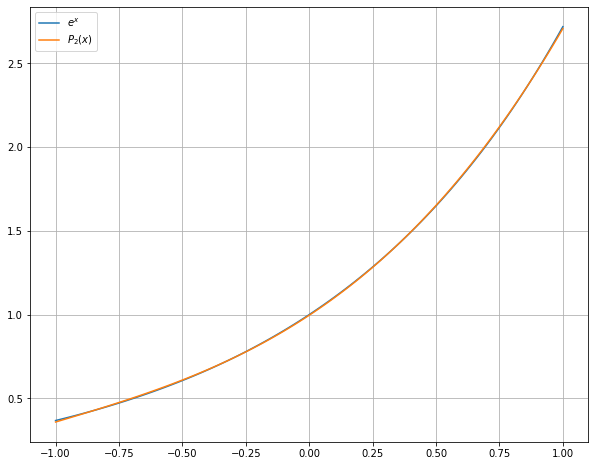
\includegraphics[width=0.8\textwidth]{p1poly3.png}
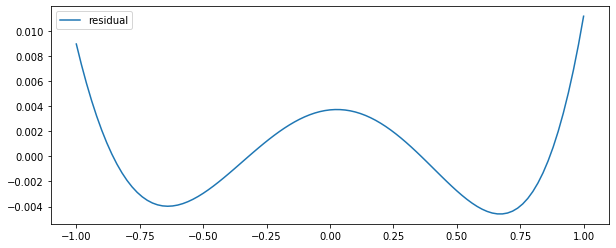
\includegraphics[width=0.8\textwidth]{p1poly3_res.png}
\end{figure}


\newpage
\subsection{Chebyshev Polynomial Identity}
Show that:
$$
	T_i(x)T_j(x) =\frac12 (T_{i+j}(x) + T_{i-j}(x)), \forall i>j
$$
\subsubsection{}
WLOG assume $i\ge j$, both $i+j, i-j\ge0$. Would like to show for Chebyshev Polynomials:
$$
	T_i\cdot T_j = \frac12 (T_{i+j} + T_{i-j})
$$

We use a trigonometric identity:
$$
\cos(a+b) = \cos(a)\cos(b) - \sin(a)\sin(b)
$$
$$
	\cos(a-b) = \cos(a)\cos(b) + \sin(a)\sin(b)
$$ therefore we have:
$$
	\cos(a)\cos(b) = \frac12(\cos(a+b) + \cos(a-b))
$$

By definition of Chebyshev Polynomial:
$$
	T_i(x)\cdot T_j(x) = \cos(i\arccos(x))\cdot \cos(j\arccos(x)) 
$$
$$= \frac{1}{2}\bigg[
	\cos((i+j)\arccos(x) + \cos((i-j)\arccos(x)))
	\bigg] = \frac12(T_{i+j}(x) + T_{i-j}(x))
$$ as desired.

\subsubsection{other properties of Chebyshev Polynomials}
The following can be proved using the definition, recurrence relation, and previous properties (let us know if you attempted the proofs!).

(1)
$$
	T_n(1) = 1
$$

(2)
$$
	T_n(x) = 2^{n-1}x^n + O(x^{n-1})
$$

(3)
$$
	T_n(x) = 
	\begin{cases}
		\cos(n\cdot \arccos(x)), \text{ if }\abs{x}\le 1\\
		\cosh(n\cdot \arccosh(x)), \text{ if }\abs{x}\ge 1
	\end{cases}
$$

(4)
$$
	\text{ if }\abs{x}\le 1, \abs{T_n(x)}\le 1
$$

(5)
$$
	T_n(x) = \frac12 \big[
	(x+\sqrt{x^2-1})^m + (x + \sqrt{x^2 - 1})^{-m}
	\big], \text{ for}\abs{x}> 1
$$

(6)
$$
	T_n(1+\eps) \ge \frac12(1+n\sqrt{2\eps}),\text{ for }\eps>0
$$


\newpage
\subsection{Laguerre Polynomial Recurrence Relation}
Derive the 3-term recurrence relation for the Laguerre polynomials $L_n$, which are orthogonal with respect to the weight function $w(x) = e^{-x}$ on the interval $(0,\infty)$. Plot the polynomials $L_0, L_1,L_2,L_3$ on an interval containing all of their respect zeros, discuss interlacing of roots. 
\subsubsection{}
The derivation of Laguerre Polynomial recurrence is graded, but lightly. The proof follows from plugging in $B_k, C_k$ and verifying the general formula for (normalized) Laguerre polynomials (cannot use the recurrence in Theorem 8.7 directly without proof).

The general formula for Laguerre polynomials is:
$$
	L_k(x) = \sum_{j=0}^{k}{k\choose j}\frac{(-1)^j}{j!}x^j
$$ yielding the recurrence:
$$
	(k+1)L_{k+1}(x) = (2k+1-x)L_{k}(x) - kL_{k-1}(x)
$$

Computations:

Let:
$$
	L_0(x) = 1, w(x) = e^{-x}
$$ we use Theorem 8.7 from textbook to construct polynomials of higher degrees with domain $(0,\infty)$. 
$$
	B_1 = \frac{\int_0^{\infty} xe^{-x}dx}{\int_0^{\infty} e^{-x}dx} = \frac{1}{1}= 1
$$
$$
	L_1(x) = x-1
$$

For $n=2$:
$$
	B_2 = \frac{\int_0^{\infty} xe^{-x}(x-1)^2dx}{\int_0^{\infty}e^{-x}(x-1)^2dx} = \frac{3}{1} = 3
$$
$$
	C_2 = \frac{\int_0^{\infty} xe^{-x}(x-1)dx}{\int_0^{\infty} e^{-x}dx} = \frac{1}{1} = 1
$$
$$
	L_2(x) = (x-3)(x-1) - 1 = x^2-4x+2
$$

For $n=3$:
$$
	B_3 = \frac{\int_0^{\infty} xe^{-x}(x^2-4x+2)^2dx}{\int_0^{\infty} e^{-x}(x^2-4x+2)^2dx} = \frac{20}{4} = 5
$$
$$
	C_3 = \frac{\int_0^{\infty} xe^{-x}(x^2-4x+2)(x-1)dx}{\int_0^{\infty} e^{-x}(x-1)^2dx} = \frac{4}{1} = 4
$$
$$
	L_3(x) = (x-5)\cdot (x^2-4x+2)-4(x-1) = x^3-9x^2+18x-6
$$

Numerical solutions:

$L_0$ has no zeros. 

For $L_1$, $x_1^{(1)} = 1$.

For $L_2$, $x_2^{(1)} \approx 0.58579, x_2^{(2)} \approx 3.41421$.

For $L_3$, $x_3^{(1)} \approx 0.41577, x_3^{(2)} \approx 2.29428, x_3^{(3)} \approx 6.28995$. The following plot shows interlacing of zeros. In fact, this is a general property for orthogonal sequence of functions (Stieltjes interlacing property). Python code for the plot is as follows.

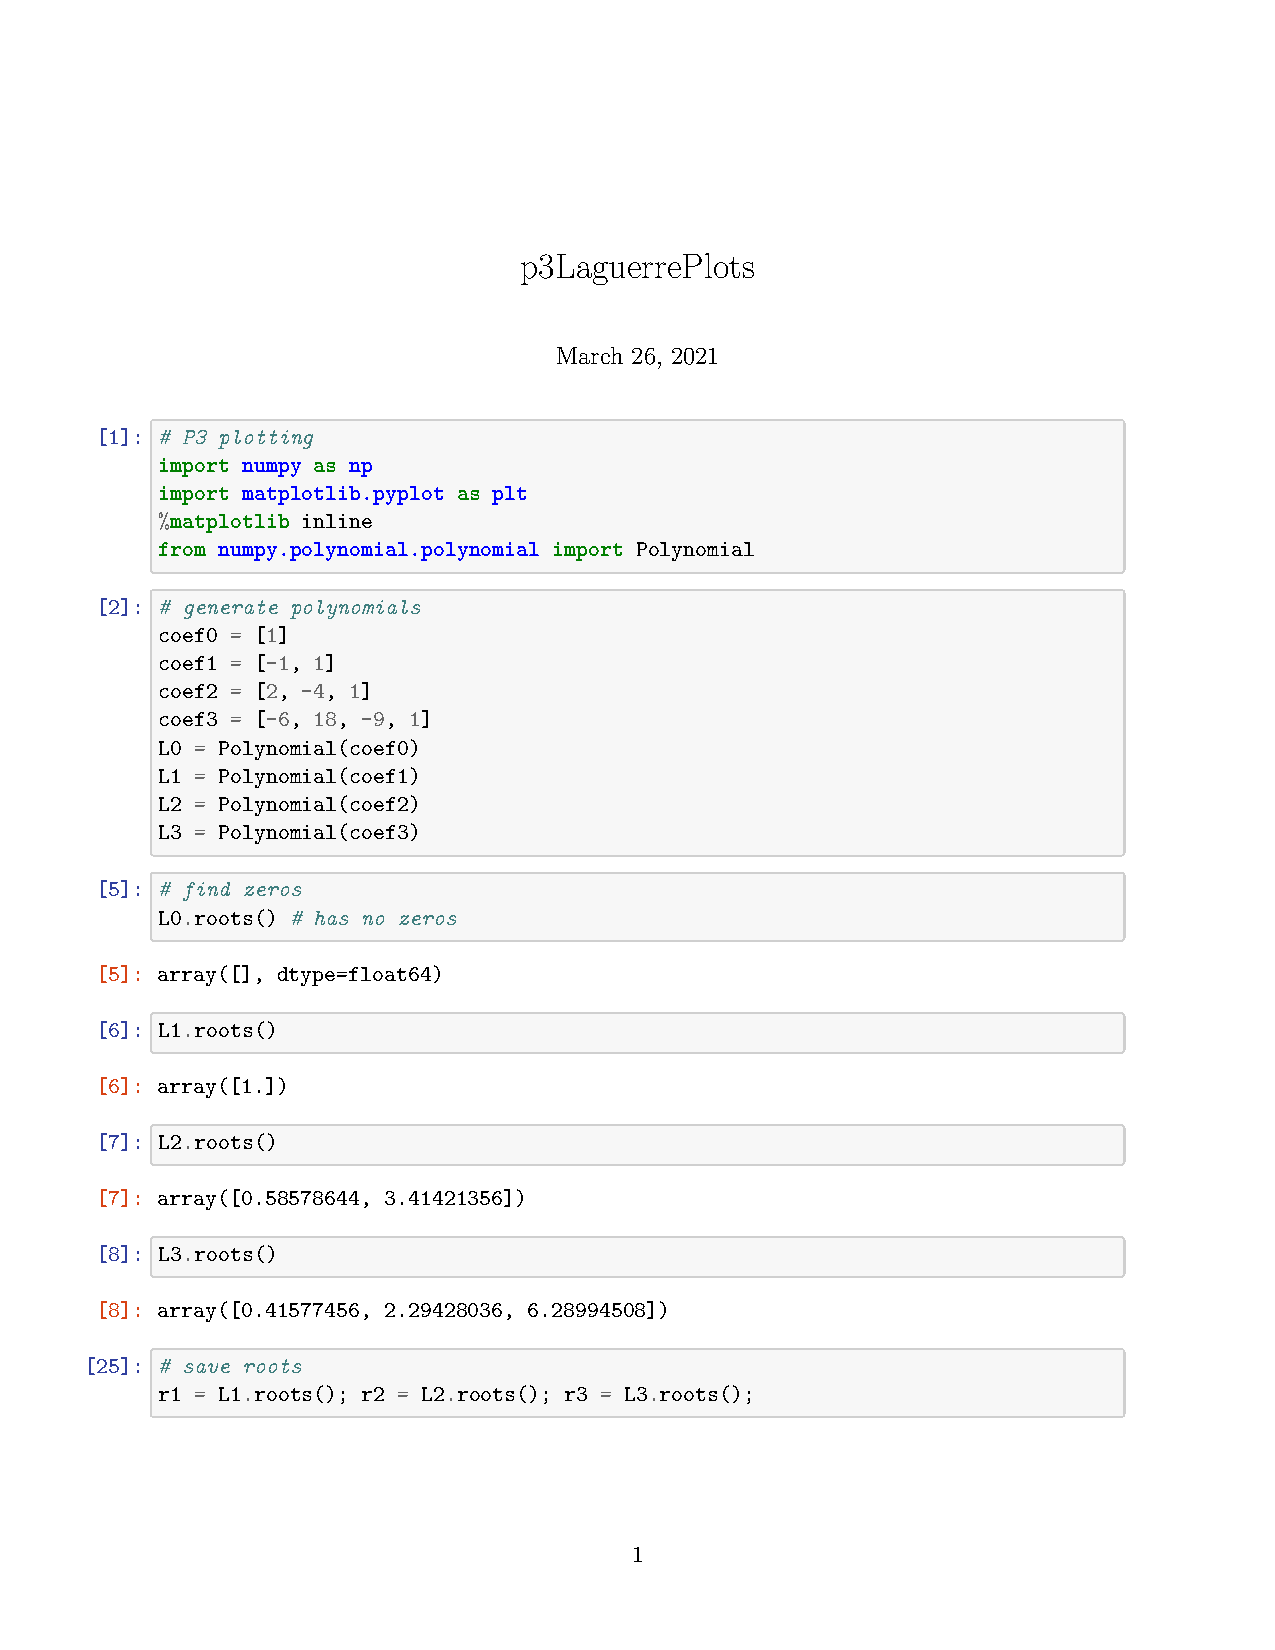
\includepdf[pages=-,pagecommand={},width=19cm]{p3LaguerrePlots.pdf}


\subsection{Padé Approximation}
Determine the Padé approximation of degree 6 with $n = 2, m=4$ to:
$$
	f(x) = \sin(x) 
$$
\subsubsection{}
The method is outlined from Page 536 to Page 538 of Textbook.

We would like to approximate:
$$
	f(x) = \sin(x) = \sum_{0}^{\infty}(-1)^i\frac{x^{2i+1}}{(2i+1)!}
$$ by solving for suitable coefficients such that (for $n=2, m=4$):
$$
	p(x) = p_2x^2+p_1x+p_0
$$
$$
	q(x) = q_4x^4 + q_3x^3 + q_2x^2 + q_1x + q_0
$$ such that:
$$
	\sum_{i=0}^ka_iq_{k-i}=p_k, k = 0,1,\cdots, 6
$$ or:
$$
	(0\cdot 1 + x +0\cdot x^2 -\frac{x^3}{6} + 0\cdot x^4+\frac{x^5}{120} + 0\cdot x^6)(1+q_1x+q_2x^2+q_3x^3+q_4x^4) 
$$
$$= p_0+p_1x+p_2x^2+0\cdot x^3 + 0\cdot x^4 + 0\cdot x^5 + 0\cdot x^6
$$

We would like all coefficients for up to $x^6$ vanish, solve:
$$
	x^0: 0 = p_0
$$
$$
	x: 1 = p_1
$$
$$
	x^2: q_1 = p_2
$$
$$
	x^3: q_2-\frac16 = 0
$$
$$
	x^4: q_3-\frac16q_1 = 0
$$
$$
	x^5: q_4 -\frac16q_2+\frac{1}{120} = 0
$$
$$
	x^6: -\frac16q_3+\frac{1}{120}q_1 = 0
$$ solving this system yields:
$$
	\begin{cases}
		p_0 = 0\\
		p_1 = 1\\
		p_2 = 0\\
		q_0 = 1\\
		q_1 = 0\\
		q_2 = \frac16\\
		q_3 = 0\\
		q_4 = \frac{7}{360}
	\end{cases}
$$
$$
	p(x) =x,
	q(x) = \frac{7}{360}x^4 + \frac16x^2 + 1
$$ thus the rational approximant is:
$$
	r(x) = \frac{x}{\frac{7}{360}x^4 + \frac16x^2 + 1}
$$

The following page contains a plot to verify our intuition that it should approximate $f(x) = \sin(x)$ well around $x=0$.

\begin{figure}[h]
\centering
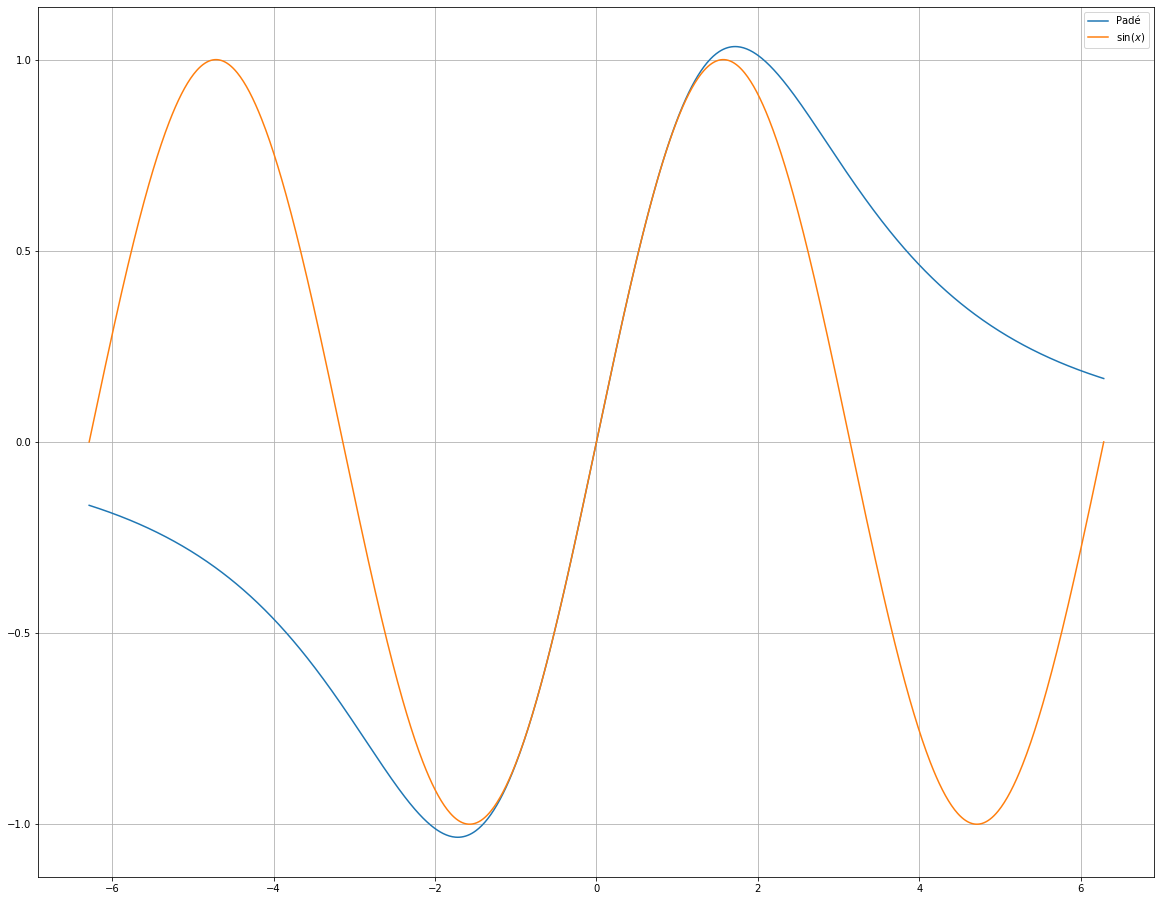
\includegraphics[width=0.8\textwidth]{p4PadePlot.png}
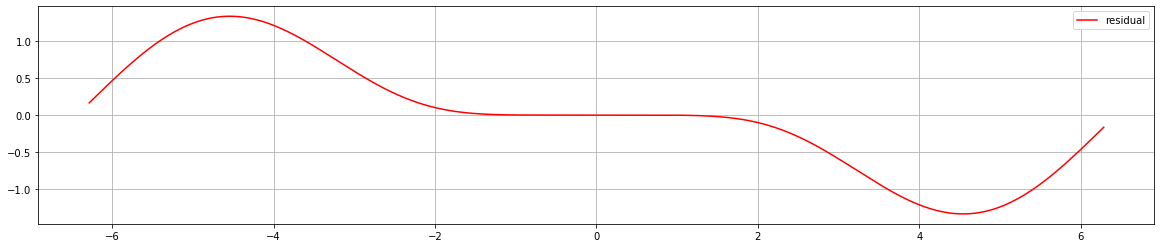
\includegraphics[width=0.8\textwidth]{p4PadeResidual.png}
\end{figure}


\newpage
\subsection{Cont'd Fractions for Rational Functions}
Express the following rational functions as continued fractions:
$$
	f_1(x) = \frac{4x^2 + 3x-7}{2x^3 + x^2- x +5}, f_2(x) = \frac{2x^3 +x^2 +3x-1}{3x^3 + x^2 - x+1}
$$
\subsubsection{}
Continued fraction is of the form:
$$
	(a_0x+b_0) + \frac{c_1}{(a_1x+b_1) + \frac{c_2}{(a_2x+b_2) + \frac{c_3}{(a_3x+b_3) + \ddots}}}
$$ whose primary use is to reduce the number of flops or express irrational numbers.

Each step of continued fraction is done by doing polynomial long division. The choice of scaling in this solution is purely for convenience of computations. Student answer is considered correct up to scaling of both numerator and denominator with suitable constants. 
\subsection{a}
$$
	\frac{4x^2 + 3x - 7}{2x^3 + x^2 - x + 5} = \frac{1}{\frac{2x^3 + x^2 - x + 5}{4x^2 + 3x - 7}} = \frac{8}{\frac{16x^3 + 8x^2 -8x +40}{4x^2 +3x-7}} 
$$
$$= 
	\frac{8}{(4x-1) + \frac{23x+33}{4x^2+3x-7}} = 
	\frac{8}{(4x-1) + \frac{529}{(92x-63) - \frac{1624}{23x+33}}}
$$

\subsection{b}
$$
	\frac{2x^3+x^2+3x-1}{3x^3+x^2-x+1} = \frac13\cdot\frac{6x^3+3x^2+9x-3}{3x^3+x^2-x+1} = 
	\frac13\bigg(
	2+\frac{x^2+11x-5}{3x^3+x^2-x+1}
	\bigg)
$$
$$
	=\frac23 + \frac{x^2+11x-5}{9x^3+3x^2-3x+3} = \frac23+\frac{1}{\frac{9x^3+3x^2-3x+3}{x^2+11x-5}}
$$
$$
= \frac23+\frac{1}{(9x-96)+\frac{1098x-477}{x^2+11x-5}} = 
\frac23+\frac{1}{(9x-96)+\frac{1}{\frac{x^2+11x-5}{1098x-477}}}
$$
$$
	= \frac23+\frac{1}{(9x-96)+\frac{1098}{\frac{1098x^2+12078x-5490}{1098x-477}}} = \frac23+\frac{1}{(9x-96)+\frac{1098}{(x+\frac{12555}{1098}) - \frac{\frac{39285}{1098}}{1098x-477}}}
$$

\newpage
% begin HW8
\section{Homework 8}
\subsection{Trigonometric Approximation}
Find the continuous least squares trigonometric polynomial $S_n$ for:
$$
	f(x) = e^x
$$ on the interval $[-\pi, \pi]$.
\subsubsection{}

Find continuous least squares trigonometric polynomial approximation for $f(x) = e^x$ on $[-\pi,\pi]$. 

\emph{Remark}
The root for this kind of approximation is the {\color{black} Stone-Wierstrass approximation}, a special case shows that trigonometric polynomials are \emph{dense} in the space of continuous functions. An intuitive understanding of \emph{dense}, without reproducing the exact definition is to consider the analogy that $\mathbb{Q}$ is dense in $\rr$. For any arbitrary real number, we can find an arbitrarily good approximation of that real number in $\mathbb{Q}$. Similarly, for any continuous function, we can find an arbitrarily good approximation of that function using trig polynomials. 

Using Textbook notation in Sect. 8.5, the general form is:
$$
	S_n(x) = \frac12a_0 + a_n\cos nx + \sum_{k=1}^{n-1}(a_k\cos kx + b_k\sin kx)
$$

Doing the computations yields:
$$
	a_0 = \frac{1}{\pi}\int_{[-\pi,\pi]}e^xdx = \frac{1}{\pi}(e^{\pi} - e^{-\pi})
$$

$$
	a_k = \frac{1}{\pi}\int_{[-\pi,\pi]}f(x)\cos kxdx = \frac{1}{\pi}\int_{[-\pi,\pi]}e^x\cos(kx)dx
$$
$$
	= \frac{1}{\pi}\cdot\frac{e^x(k\sin(kx) + \cos(kx))}{k^2+1}\big|_{-\pi}^{\pi} = \frac{(-1)^k\cdot k }{(k^2+1)\pi}(e^{\pi}-e^{-\pi})
$$ because $\sin(-k\pi) = \sin(k\pi) = 0, k \in \nn$, $\cos(k\pi)=\cos(-k\pi) = \pm 1$.
$$
	b_k =\frac{1}{\pi} \int_{[-\pi,\pi]}f(x)\sin kxdx = \frac{1}{\pi} \int_{[-\pi,\pi]}e^x\sin kxdx=\frac{1}{\pi}\bigg(
	\frac{e^x(\sin(kx) - k\cos(kx))}{k^2+1}\big|_{-\pi}^{\pi}
	\bigg)
$$
$$
	= \frac{(-1)^k\cdot k }{(k^2+1)\pi}(e^{-\pi}-e^{\pi})
$$


\subsection{Degree-4 Discrete Least Squares Trig Approximation}
Determine the discrete least squares trigonometric polynomial $S_4$ for $f(x) = e^x$ on $[-\pi,\pi]$, and compute the error $E_4(x)$ of this approximation.
\subsubsection{}
Theorem 8.13 in Textbook gives the explicit formula for computing the approximation. The Python code below is used to generate and plot these polynomials. 

With regression methods, $m$ controls the number of data points we are fitting on. For a fixed $n$, increasing $m$ will keep decreasing error for some time. If $m$ is too large, however, we start to see \emph{overfitting}. The code file is also uploaded to Resources if you would like to run it with different parameter choices.

The coefficients are given explicitly:
$$
	a_k = \sum_{0}^{2m-1}y_j\cos(kx_j), k\in \{0,1, 2,\cdots, n\}
$$
$$
	b_k = \sum_{0}^{2m-1}y_j\sin(kx_j), k\in \{0,1, 2,\cdots, n-1\}
$$

The coefficients for $n=4, m=2n-1=7$ found using the code on the following page are:
\begin{verbatim}
a_coef = [ 5.82532985, -2.15048477, 
-0.05134437,  0.77977417, -1.07202048]

b_coef = [ 3.55350809, -2.69329961,  1.82801647]
\end{verbatim}

With total squared error: 42.3402344921022.


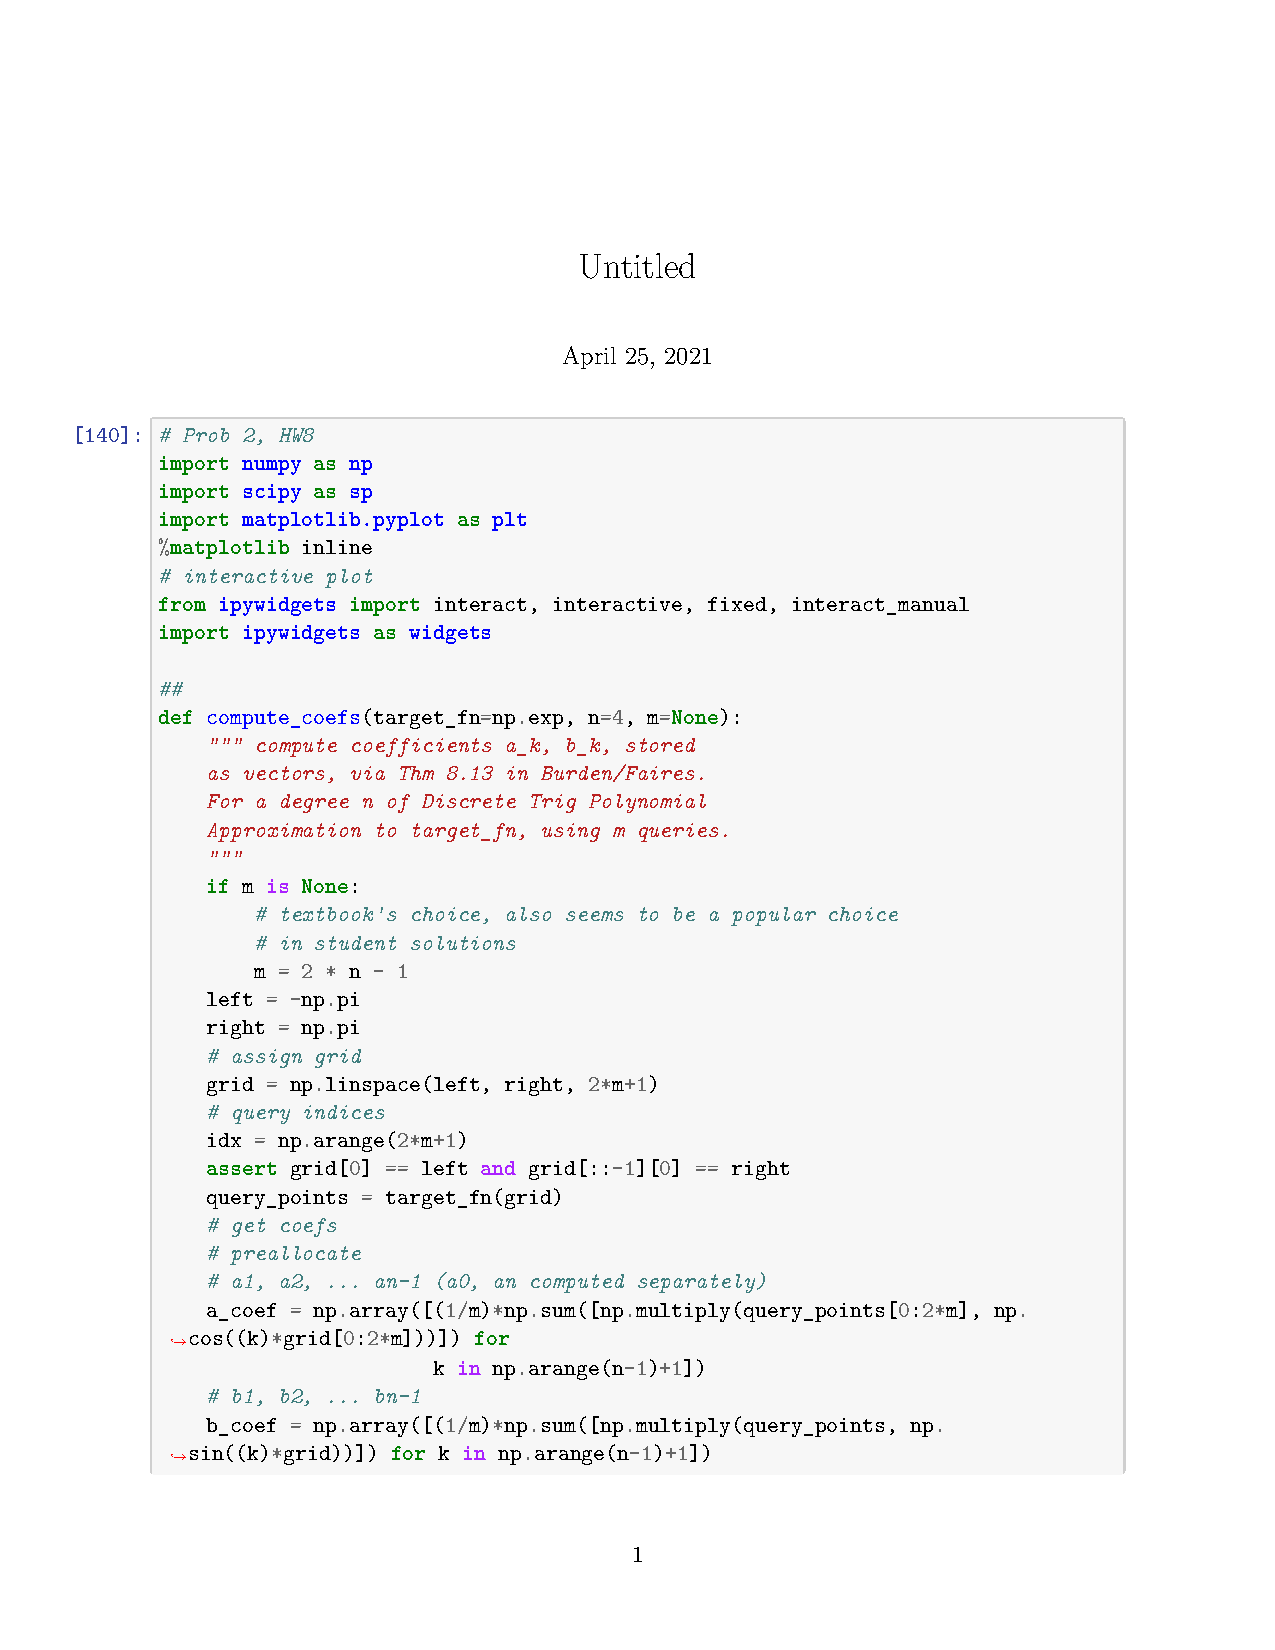
\includepdf[pages=-,pagecommand={},width=18cm]{hw8_Untitled.pdf} 


\subsection{Trigonometric interpolating polynomial}
Determine the trigonometric interpolating polynomial of degree 4 for $f(x) = x(\pi - x)$ on $[-\pi,\pi]$ using direct calculation and FFT, respectively.
\subsubsection{direct calculation}
Direct calculation used the Python code from Problem 2, with:
$$
	f(x) = -x^2 + \pi x, x\in [-\pi,\pi]
$$

To replicate the results, open 
\begin{verbatim}
hw8_p2_slider.ipynb
\end{verbatim} and run:
\begin{verbatim}
approximate(target_fn=lambda x: x*(np.pi-x), n=4, verbose=True)
\end{verbatim}

\begin{figure}[h]
\caption{4-th Degree approximation of $x(\pi -x)$}
\centering
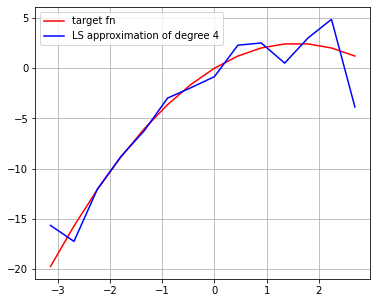
\includegraphics[width=0.6\textwidth]{p3_direct.png}
\end{figure}

\subsubsection{Fast Fourier Transform}
The illustration in Section 8.6 and Algorithm 8.3 provide an explanation of the implementation. For a demo, we use $8=2\cdot 2^2$ data points on $[-\pi, \pi]$, namely:
$$
	x_j = -\pi+\frac{j\pi}{4}, j = 0,1,2,\cdots, 7
$$

We seek the approximation:
$$
	S_4(x) = 
	\frac{1}{2}a_0 + \frac{1}{2}a_4\cos(4x) + \sum_{k=1}^3(a_k\cos(kx) + b_k\sin(kx))
$$

By formula, the FFT is defined as:
$$
	\frac{1}{4}\sum_{j=0}^7 c_ke^{ikx}
$$ where:
$$
	c_k = \sum_{j=0}^7y_je^{ik\pi j/4}
$$

Then direct calculation gives:
$$
	c_0 = \sum_0^7 y_i
$$
$$
	c_1 = y_0+(\frac{i+1}{\sqrt{2}})y_1 + iy_2+(\frac{i-1}{\sqrt{2}})y_3 - y_4- (\frac{i+1}{\sqrt{2}})y_5-iy_6 -(\frac{i-1}{\sqrt{2}})y_7
$$
$$
	c_2 = y_0 + iy_1 - y_2 -iy_3 +y_4 + iy_5 - y_6-iy_7
$$
$$
	c_3 = y_0+(\frac{i-1}{\sqrt{2}})y_1 - iy_2+(\frac{i+1}{\sqrt{2}})y_3 - y_4- (\frac{i-1}{\sqrt{2}})y_5+iy_6 -(\frac{i+1}{\sqrt{2}})y_7
$$
$$
	c_4 = y_0 - y_1 + y_2 -y_3 +y_4 -y_5 + y_6-y_7
$$
$$
	c_5 = y_0-(\frac{i+1}{\sqrt{2}})y_1 + iy_2-(\frac{i-1}{\sqrt{2}})y_3 - y_4+ (\frac{i+1}{\sqrt{2}})y_5-iy_6 +(\frac{i-1}{\sqrt{2}})y_7
$$
$$
	c_6 = y_0 - iy_1 - y_2 +iy_3 +y_4 -iy_5 - y_6+iy_7
$$
$$
	c_7 = y_0-(\frac{i-1}{\sqrt{2}})y_1 - iy_2-(\frac{i+1}{\sqrt{2}})y_3 - y_4+ (\frac{i-1}{\sqrt{2}})y_5+iy_6 +(\frac{i+1}{\sqrt{2}})y_7
$$

The above expressions are from Page 559 of textbook. Page 560 has a further explanation of reducing flops. If we implement a double for loop to compute the $c_k$, there is no advantage; the written part is only a demonstration.

With the help of a calculator we obtain (rounded to 2 decimals):
$$
	c_0 = -37.01, c_1 = -26.72-23.83i, c_2 =-14.8-13.57i
$$
$$
	c_3 = -12.76-4.09i, c_4 = -12.34, c_5 = -12.76+4.09i
$$
$$
	c_6 = -14.8+9.87i, c_7 = -26.72+23.83i
$$

Now we can set up the coefficients as:
$$
	a_k = \Re(\frac{1}{4}c_ke^{-ik\pi})
$$
$$
	b_k = \Im(\frac{1}{4}c_ke^{-ik\pi})
$$ for $k = 0,1,2,3,4$.

Now we recover:
$$
	a_0 = -9.25275413, a_1 = 6.67951825, a_2 = -3.70110165
$$
$$
	a_3 = 3.19008615, a_4 = -3.08425138
$$
$$
	b_0 = 0, b_1 = 5.9568332, b_2 = -3.39267651
$$
$$
	b_3 = 1.022031, b_4 = 0
$$

The following is a plot of the approximation using these coefficients.

\begin{figure}[h]
\caption{4-th Degree approximation of $x(\pi -x)$ via FFT}
\centering
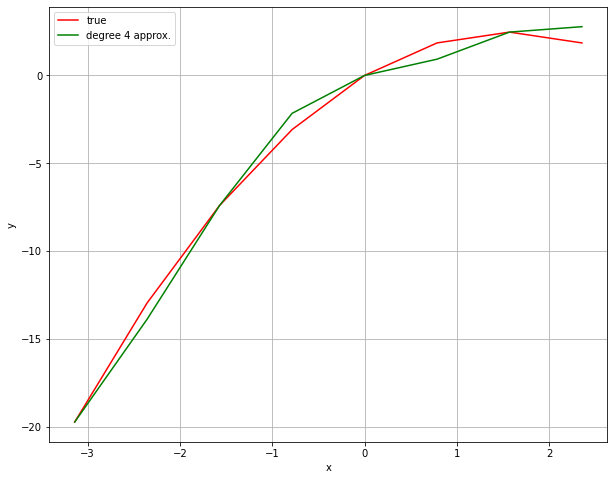
\includegraphics[width=0.6\textwidth]{hw8p3b.png}
\end{figure}





\newpage
\subsection{Equivalent Matrix Vector Multiply}
Show that $c_0, \cdots, c_{2m-1}$ in B\& F Algorithm 8.3 is given by:
$$
	\begin{pmatrix}
		c_0 \\
		c_1 \\
		c_2 \\
		\vdots\\
		c_{2m-1}
	\end{pmatrix} = 
	\begin{pmatrix}
		1 & 1 & 1 & \cdots & 1 \\
		1 & \omega & \omega^2 & \cdots & \omega^{2m-1} \\
		1 & \omega^2 & \omega^4 & \cdots & \omega^{4m-2} \\
		\vdots & \cdots & \cdots & \ddots & \vdots  \\
		1 & \omega^{2m-1} & \omega^{4m-2} & \cdots & \omega^{(2m-1)^2}
	\end{pmatrix} \cdot
	\begin{pmatrix}
		y_0 \\
		y_1\\
		y_2\\
		\vdots\\
		y_{2m-1}
	\end{pmatrix}
$$ where $\omega = e^{\pi i/m}$. Also, find the eigenvalues of this matrix.
\subsubsection{Matrix Vector Equivalence}
Refer to equation (8.28) in Textbook:
$$
	c_k = \sum_{j=0}^{2m-1}y_je^{ik\pi j/m}, k=0,1,2,\cdots, 2m-1
$$ 

Now substitute in $\omega = e^{i\pi/m}$, then:
$$
	c_k = \sum_{j=0}^{2m-1}y_j\omega^{jk}
$$

For each $k\in\{0,1,2,\cdots, 2m-1\}$, this can be interpreted as an inner product:
$$
	c_k = \begin{pmatrix}
	1 & \omega^{k} & \omega^{2k} \cdots \omega^{(2m-1)k}
	\end{pmatrix}\cdot
	\begin{pmatrix}
	y_0\\
	y_1\\
	y_2\\
	\vdots\\
	y_{2m-1}
	\end{pmatrix}
$$

Making this substitution for every $k$ yields the desired matrix-vector product, of dimension $(2m)^2$. 
\subsubsection{Eigenvalues}
Let:
$$
	A = 
	\begin{pmatrix}
		1 & 1 & 1 & \cdots & 1 \\
		1 & \omega & \omega^2 &\cdots & \omega^{2m-1}\\
		1 & \omega^2 & \omega^4 &\cdots & \omega^{2(2m-1)}\\
		\vdots & \ddots & \cdots & \vdots& \vdots\\
		1 & \omega^{2m-1} & \omega^{(2m-1)2} &\cdots & \omega^{(2m-1)(2m-1)}
	\end{pmatrix}
$$

$A$ is the DFT matrix (the discrete Fourier transform, represented as a linear transformation; FFT refers to a computation of DFT that saves flops, hence "fast"), refer to \href{https://ieeexplore-ieee-org.libproxy.berkeley.edu/document/1163843}{this paper} to explore its properties and eigen-structure. 

The matrix:
$$
	U = \frac{1}{\sqrt{2m}}A
$$ can be proved to be a unitary matrix. Without the normalization factor $1/\sqrt{2m}$, we can show that the columns of $A$ are orthogonal.

\emph{Comment}: The proof of orthogonality is not required. If we did decide to write a proof, we need to be careful with the dot product because columns of $A$ are complex numbers:
$$
	x \cdot y = \sum_{i=0}^{2m-1}x_i\overline{y_i}
$$

Since $U$ is unitary, its determinant is 1. The eigenvalues are $\pm 1, \pm i$. This means that the eigenvalues of $A$ are:
$$
	\pm \sqrt{2m}, \pm i\sqrt{2m}
$$

% begin HW9
\section{Homework 9}
\subsection{Fixed-Point Iteration for Nonlinear System}
Use fixed point iteration to find all solutions to the nonlinear system outlined below, to accuracy within $O(10^{-5})$, and use $l_{\infty}$-norm.
\subsubsection{}
The system:
$$
	x_1^2 + x_2^2 - x_1 = 0
$$
$$
	x_1^2 - x_2^2 - x_2 = 0
$$ has 2 real solutions.

By rearranging:
$$
	x_2 = \pm\sqrt{-x_1^2+x_1}
$$
$$
	x_2 = -\frac12\pm \sqrt{x_1^2 + \frac14}
$$

Then we can plot $x_2$ against $x_1$ and look at the intersections, as shown below (we need to restrict the domain to $x_1\in [0,1]$, otherwise, complex solutions will arise for the circle part, but we are operating in $\rr^2$; having more than 2 solutions is not incorrect, only the 2 real solutions are graded):

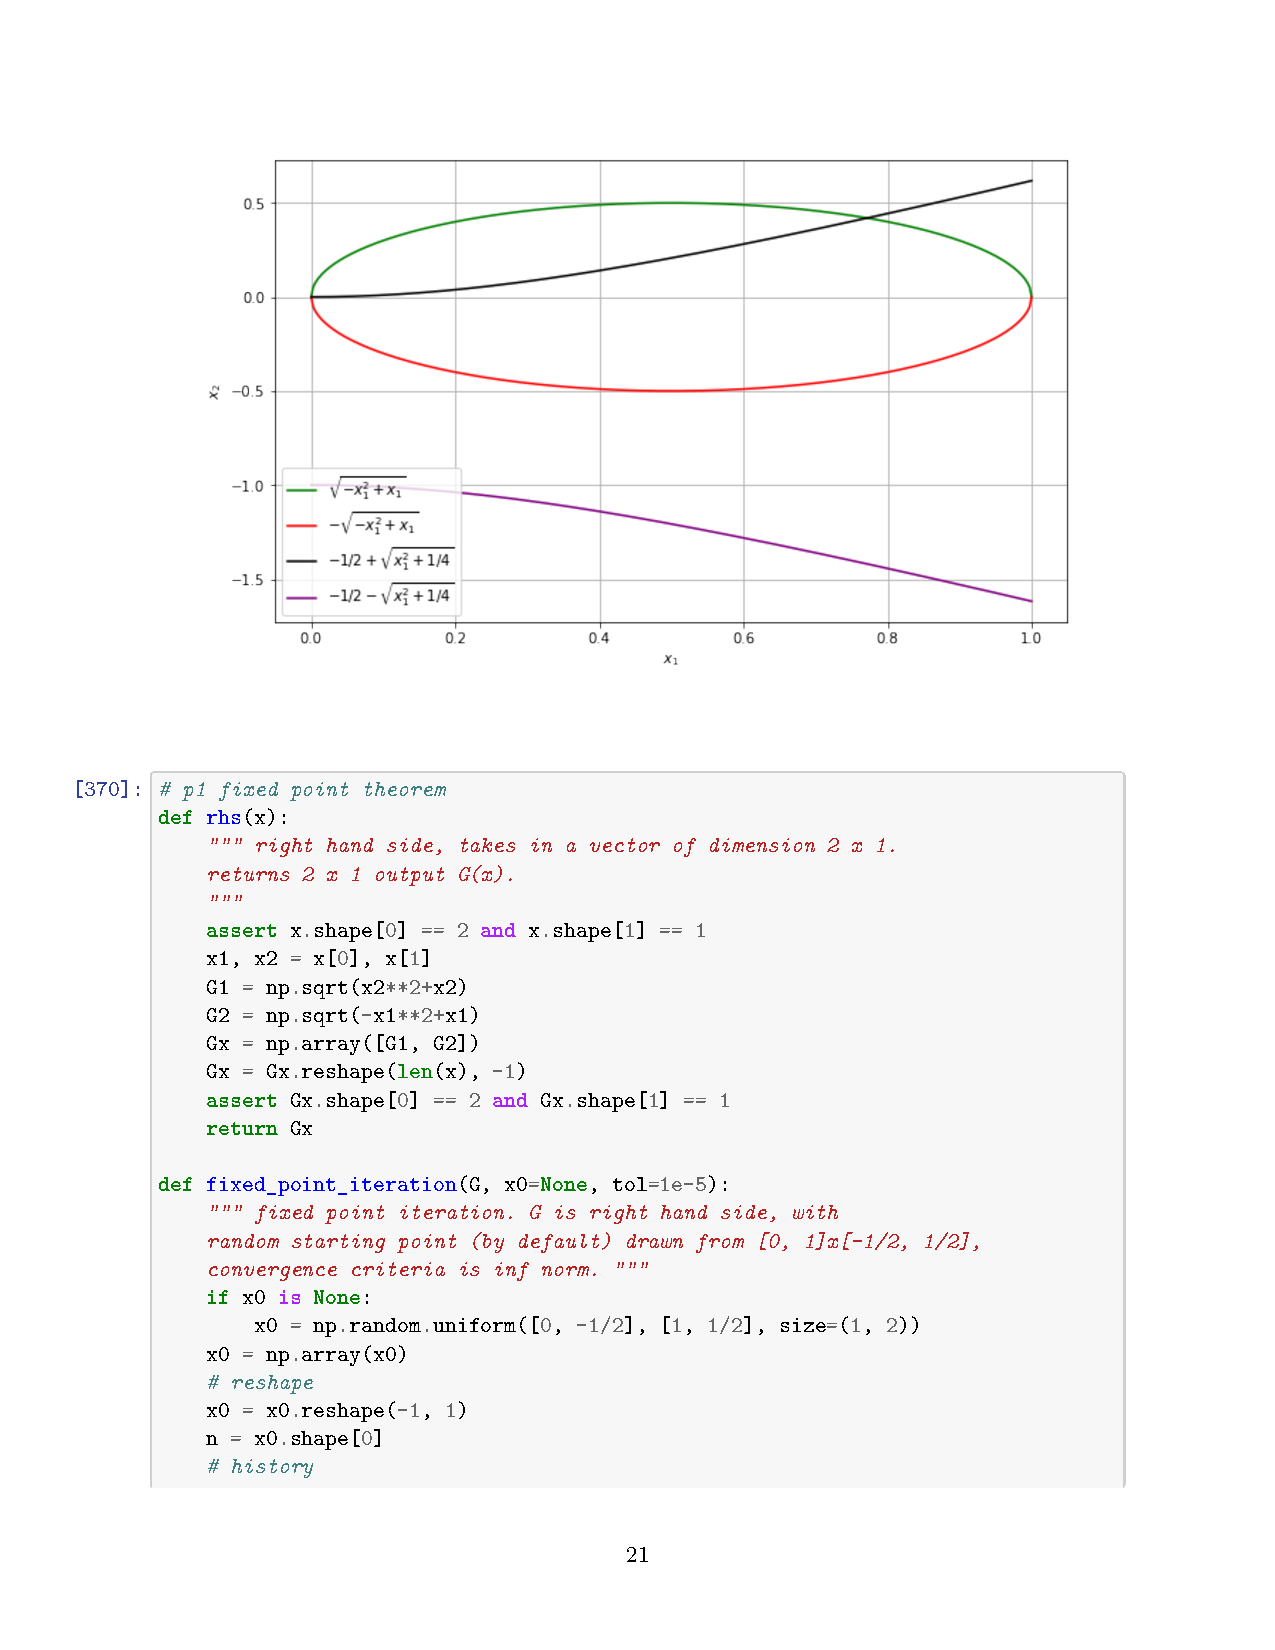
\includepdf[pages=-]{p1.pdf}
Another solution is found by setting $\mathbf{x_0} = (\eps, \eps)^T$ where $\eps \approx 0$; this will yield $\mathbf{x} = (0,0)^T$.

Rearrange and solve for $x_1$, $x_2$, using the appropriate branch of the $x_1$ circle and the $x_2$ parabola:
$$
	x_1 = \sqrt{x_2^2+x_2}
$$
$$
	x_2 = \sqrt{-x_1^2 + x_1}
$$

Now let $D=\{(x_1, x_2): x_1\in[0,1],x_2\in[-1/2, 1/2]\}$ be a rectangle, where our solutions lie:
$$
	\mathbf{G}(\mathbf{x}) = 
	\begin{pmatrix}
		\sqrt{x_2^2+x_2} \\
		\sqrt{-x_1^2 + x_1}
	\end{pmatrix}
$$ then compute the Jacobian matrix:
$$
	\mathbf{J} = 
	\begin{pmatrix}
		\frac{\partial G_1}{\partial x_1} & \frac{\partial G_1}{\partial x_2}\\
		\frac{\partial G_2}{\partial x_1} & \frac{\partial G_2}{\partial x_2}
	\end{pmatrix}
	=
	\begin{pmatrix}
	0 & \frac12(x_2^2+x_2)^{-1/2}\cdot(2x_2+1)\\
	-\frac12(-x_1^2+x_1)^{-1/2}\cdot (2x_1-1) & 0
	\end{pmatrix}
$$ due to the $-1/2$ power, we see that it is not bounded by some constant less than 1 in the original $D$, however this can be mitigated and solved by restricting the domain away from $x_1=0$; in the smaller domain, the fixed point is unique and independent of starting points 

\emph{Comment}: many students concluded at this point that there does not exist any solutions / the fixed point iteration does not converge. Theorem 10.6 has two parts. One, a fixed point \emph{exists} if $\mathbf{G}$ is a continuous, injective map into $D$. Part two is a stronger condition about whether we will always converge to a unique fixed point regardless of choice of starting points.





\newpage
\subsection{Continuous Differentiability}
Let $A$ be $\rr^{n\times n}$ and define the operator:
$$
	F: \rr^{n}\rightarrow \rr^n
$$ with:
$$
	F(x) = Ax
$$ 

Show that $F$ is continuously differentiable on $\rr^n$. Find the Jacobian of $F$ at an arbitrary point $x\in \rr^n$.
\subsubsection{}
$F$ is a linear mapping:
$$
	F: \rr^n\rightarrow \rr^n
$$ with $F(x) = Ax$ for $A$ a constant $\rr^{n\times n}$ matrix. We need to show two parts. $F$ is differentiable, and the partial derivatives are continuous.

Recall definition of differentiability in $\rr^n\supset U\rightarrow \rr^n$. $F$ is said to be \emph{differentiable} if there exists some linear mapping $D_f$ such that:
$$
	\lim_{\norm{h}\rightarrow 0}\frac{\norm{F(\mathbf{x_0}+h) - F(\mathbf{x_0})-L(h)}}{\norm{h}}=0
$$

Refer to standard texts in Advanced Calculus for more details. Most often in proofs, we do not know what $D_f$ is \emph{a priori}. We must resort to some way of guessing. One result from calculus gives:

If all partial derivatives exist and are continuous at $\mathbf{x_0}\in U\subset \rr^n$, then $F$ is differentiable at $\mathbf{x_0}$, and the matrix representation of $L$ is uniquely given by the Jacobian (Munkres).

Therefore one good starting point is computing the Jacobian. Explicitly we can write:
$$
	F(\mathbf{x}) = A\mathbf{x} = 
	\begin{pmatrix}
		\sum_{j=1}^nA_{1j}x_j\\
		\sum_{j=1}^nA_{2j}x_j\\
		\vdots\\
		\sum_{j=1}^nA_{nj}x_j
	\end{pmatrix}
$$ then:
$$
	\frac{\partial \mathbf{F}_i}{\partial x_j} = A_{ij}
$$ since each entry of $\mathbf{F} = F(\mathbf{x})$ is a linear combination of all entries in $\mathbf{x} = (x_1,x_2,\cdots,x_n)^T$, only $x_j$ will contribute to the derivative. Furthermore, linear and constant functions in $x_j$ are continuous.

Then we have found a candidate, if we let $L(h) = Ah$, and now we have for all $\eps>0$, let $\norm{h}<\delta=\eps$, we conclude:
$$
	\frac{\norm{F(\mathbf{x_0}+h) - F(\mathbf{x_0}) - Ah}}{\norm{h}} = \frac{\norm{A\mathbf{x_0} +Ah- A\mathbf{x_0} - Ah}}{\norm{h}} = 0<\eps
$$

We conclude that $F$ is continuously differentiable, and the Jacobian is $A$. The Jacobian is the matrix representation of directional derivatives for all $\mathbf{x}\in U$ (the converse is not true, namely, all directional derivatives existing does not imply differentiability).



\subsection{Newton's Method for Nonlinear System}
Solve the following outline nonlinear system using Newton's Method, compute the first 2 iterations using $x^{(0)} = 0$.
\subsubsection{}
The nonlinear system at hand is:
$$
	\begin{cases}
		x_1^2 + x_2 - 37 = 0\\
		x_1 - x_2^2 - 5 = 0\\
		x_1 + x_2 +x_3 - 3 = 0
	\end{cases}
$$

Newton's method is introduced in Section 10.2 of Textbook, where we use the following iteration:
$$
	\mathbf{x}^{(k+1)} = \mathbf{x}^{(k)} - \mathbf{J}(\mathbf{x}^{(k)})^{-1} \cdot \mathbf{F}(\mathbf{x}^{(k)})
$$ where $\mathbf{J}$ is the Jacobian matrix, $\mathbf{F}$ comes from the system:
$$
	\mathbf{F}(\mathbf{x}) = \mathbf{0}
$$

Below is an implementation of Newton's method in Julia. 

\emph{Comment}: Many students approached the implementation of $\mathbf{J}^{-1}$ by directly inverting the Jacobian matrix. In realistic settings, direct inversion tends to be avoided because of the cost (\href{https://en.wikipedia.org/wiki/Computational_complexity_of_mathematical_operations}{{\color{blue} this}} Wikipedia page gives a reminder). A more preferred implementation (also used in Algorithm 10.1 of Textbook) is by solving the linear system for $\mathbf{y}$:
$$
	\mathbf{J}(\mathbf{x}^{(k)})(\mathbf{x}^{(k+1)} - \mathbf{x}^{(k)}) =\mathbf{J}(\mathbf{x}^{(k)})\mathbf{y}= -\mathbf{F}(\mathbf{x}^{(k)})
$$ 

Oftentimes we do not have access to $\mathbf{J}$ in closed form. Numerical Jacobian is usually found using finite differencing.

Here we have:
$$
	\mathbf{F}(\mathbf{x}) = 
	\begin{pmatrix}
		x_1^2 + x_2 - 37\\
		x_1-x_2^2 - 5\\
		x_1+x_2+x_3-3
	\end{pmatrix}
$$ and the Jacobian:
$$
	\mathbf{J}(\mathbf{x}) = 
	\begin{pmatrix}
		2x_1 & 1 & 0\\
		1 & -2x_2 & 0\\
		1 & 1 & 1
	\end{pmatrix}
$$ as expected from what we may know in Math 128A (Newton's method for 1D); this method converges roughly in second-order.

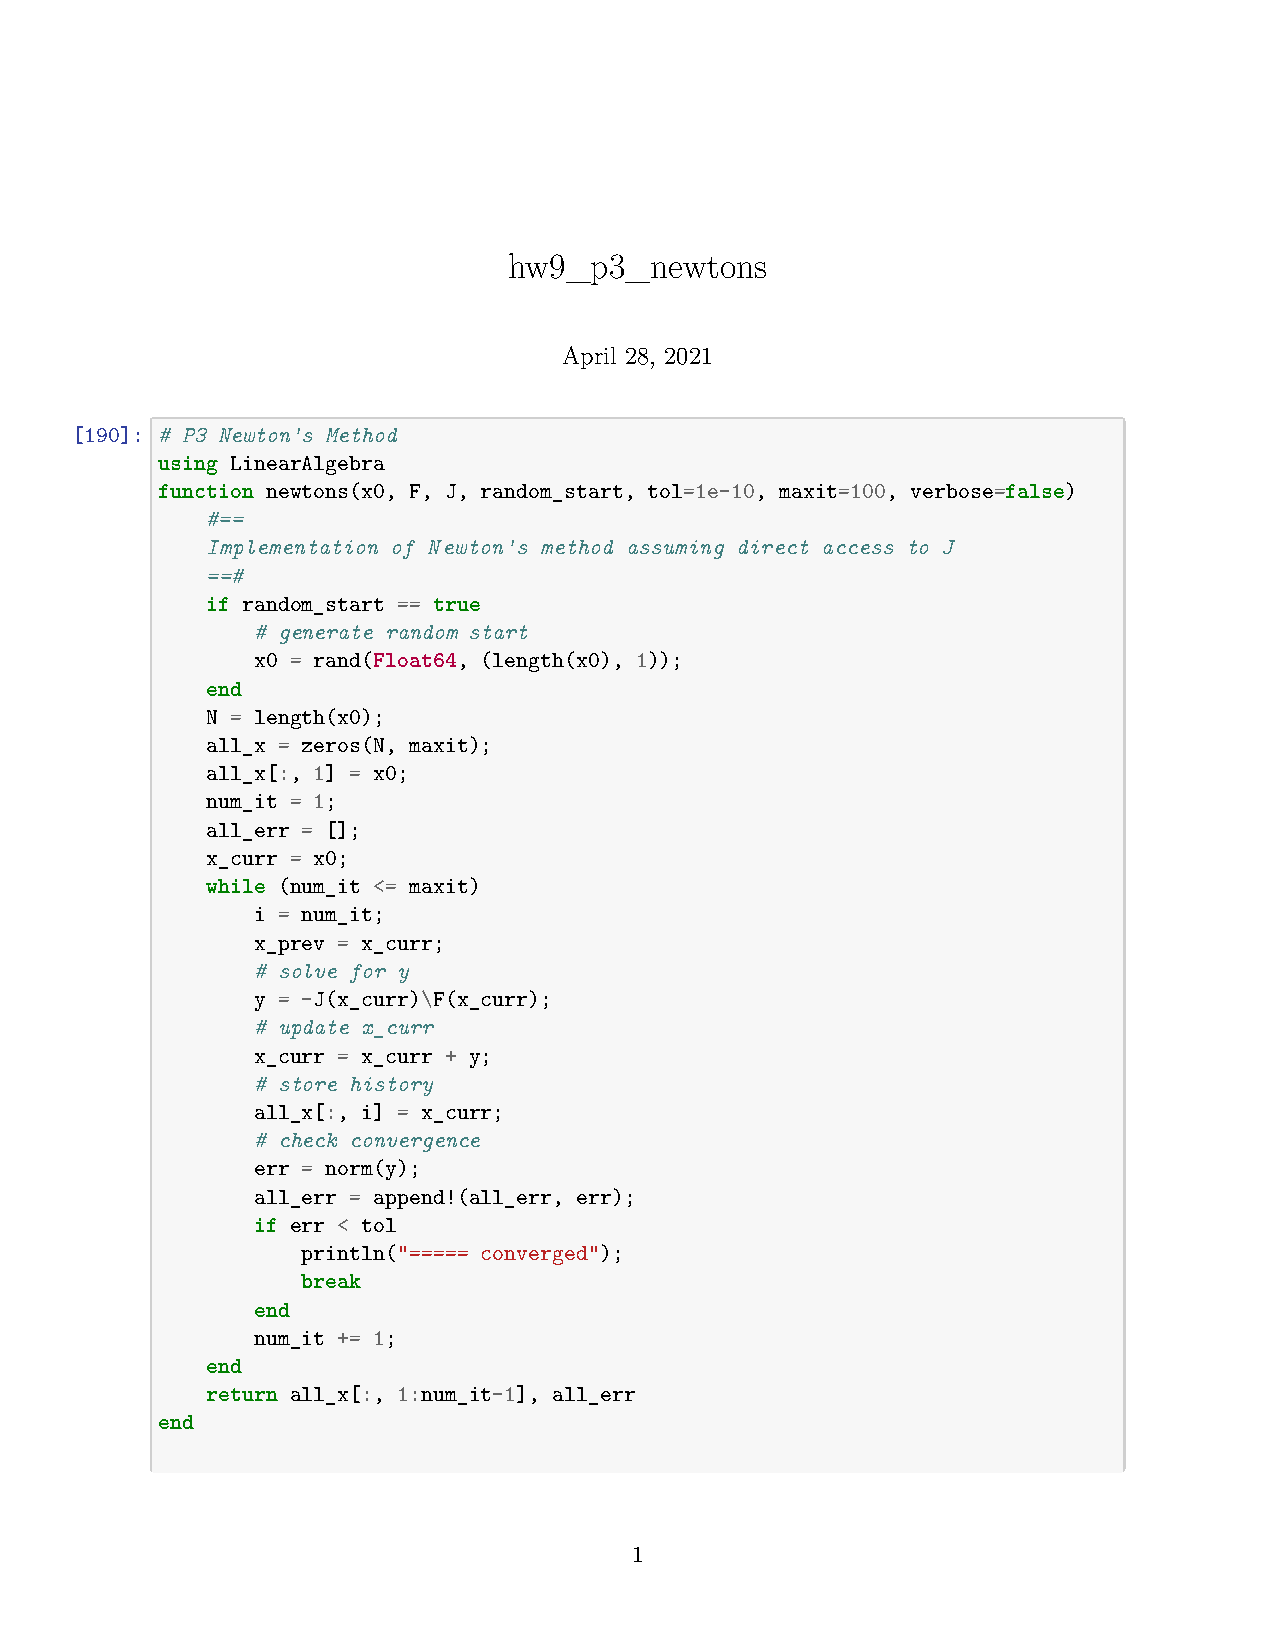
\includepdf[pages=-]{p3.pdf}

\newpage
\subsection{Nonlinear System with 6 Solutions}
Solve the following outlined nonlinear system using Broyden's method. Show that the solution is symmetric around $(x_1,x_2,x_3)$ hyperplane.
\subsubsection{}
We have the system:
$$
	\begin{cases}
		4x_1 - x_2 + x_3=x_1x_4\\
		-x_1+3x_2-2x_3 =x_2x_4\\
		x_1-2x_2+3x_3 = x_3x_4\\
		x_1^2+x_2^2+x_3^2=1
	\end{cases}
$$
\subsubsection{Symmetry}
To avoid confusion with what is known and what is unknown (the dummy variables in the system of equations), let's rename our solution to be $(a_1, a_2, a_3, a_4)^T$ which are all constants (known).

Plug in $(-a_1, -a_2, -a_3, a_4)$, we verify all equations (notice and make sense of the sign changes):
$$
-4a_1 +a_2-a_3 = -(4a_1 - a_2 + a_3) = -a_1a_4 = -(a_1)a_4
$$
$$
	-(-a_1) + 3(-a_2) - 2(-a_3) = a_1 -3a_2+2a_3 = -(-a_1+3a_2-2a_3) = -(a_2a_4) = (-a_2)a_4
$$
$$
	(-a_1) -2(-a_2)+3(-a_3) = -a_1+2a_2-3a_3 = -(a_1-2a_2+3a_3) = -(a_3a_4) = (-a_3)a_4
$$
$$
	(-a_1)^2 + (-a_2)^2+(-a_3)^2 = a_1^2+a_2^2+a_3^2=1
$$ therefore we see that it is indeed a solution.


\subsubsection{Broyden's method}
We only need to apply Broyden's method 3 times because the reflection around the $x_4$-axis is also a solution.

A Julia implementation of Algorithm 10.2 (Broyden's method) is as follows, with:
$$
	\mathbf{F}(\mathbf{x}) = 
	\begin{pmatrix}
		4x_1 - x_2 + x_3-x_1x_4\\
		-x_1+3x_2-2x_3 -x_2x_4\\
		x_1-2x_2+3x_3 - x_3x_4\\
		x_1^2+x_2^2+x_3^2-1
	\end{pmatrix}
$$ and the Jacobian:
$$
	\mathbf{J}(\mathbf{x}) = 
	\begin{pmatrix}
	4-x_4 & -1 & 1 & -x_1\\
	-1 & 3-x_4 & -2 & -x_2\\
	1 & -2 & 3-x_4 & -x_3\\
	2x_1 & 2x_2 & 2x_3 & 0
	\end{pmatrix}
$$

The solutions are on the following page, negating $x_1, x_2, x_3$ of each solutions yield new solutions.

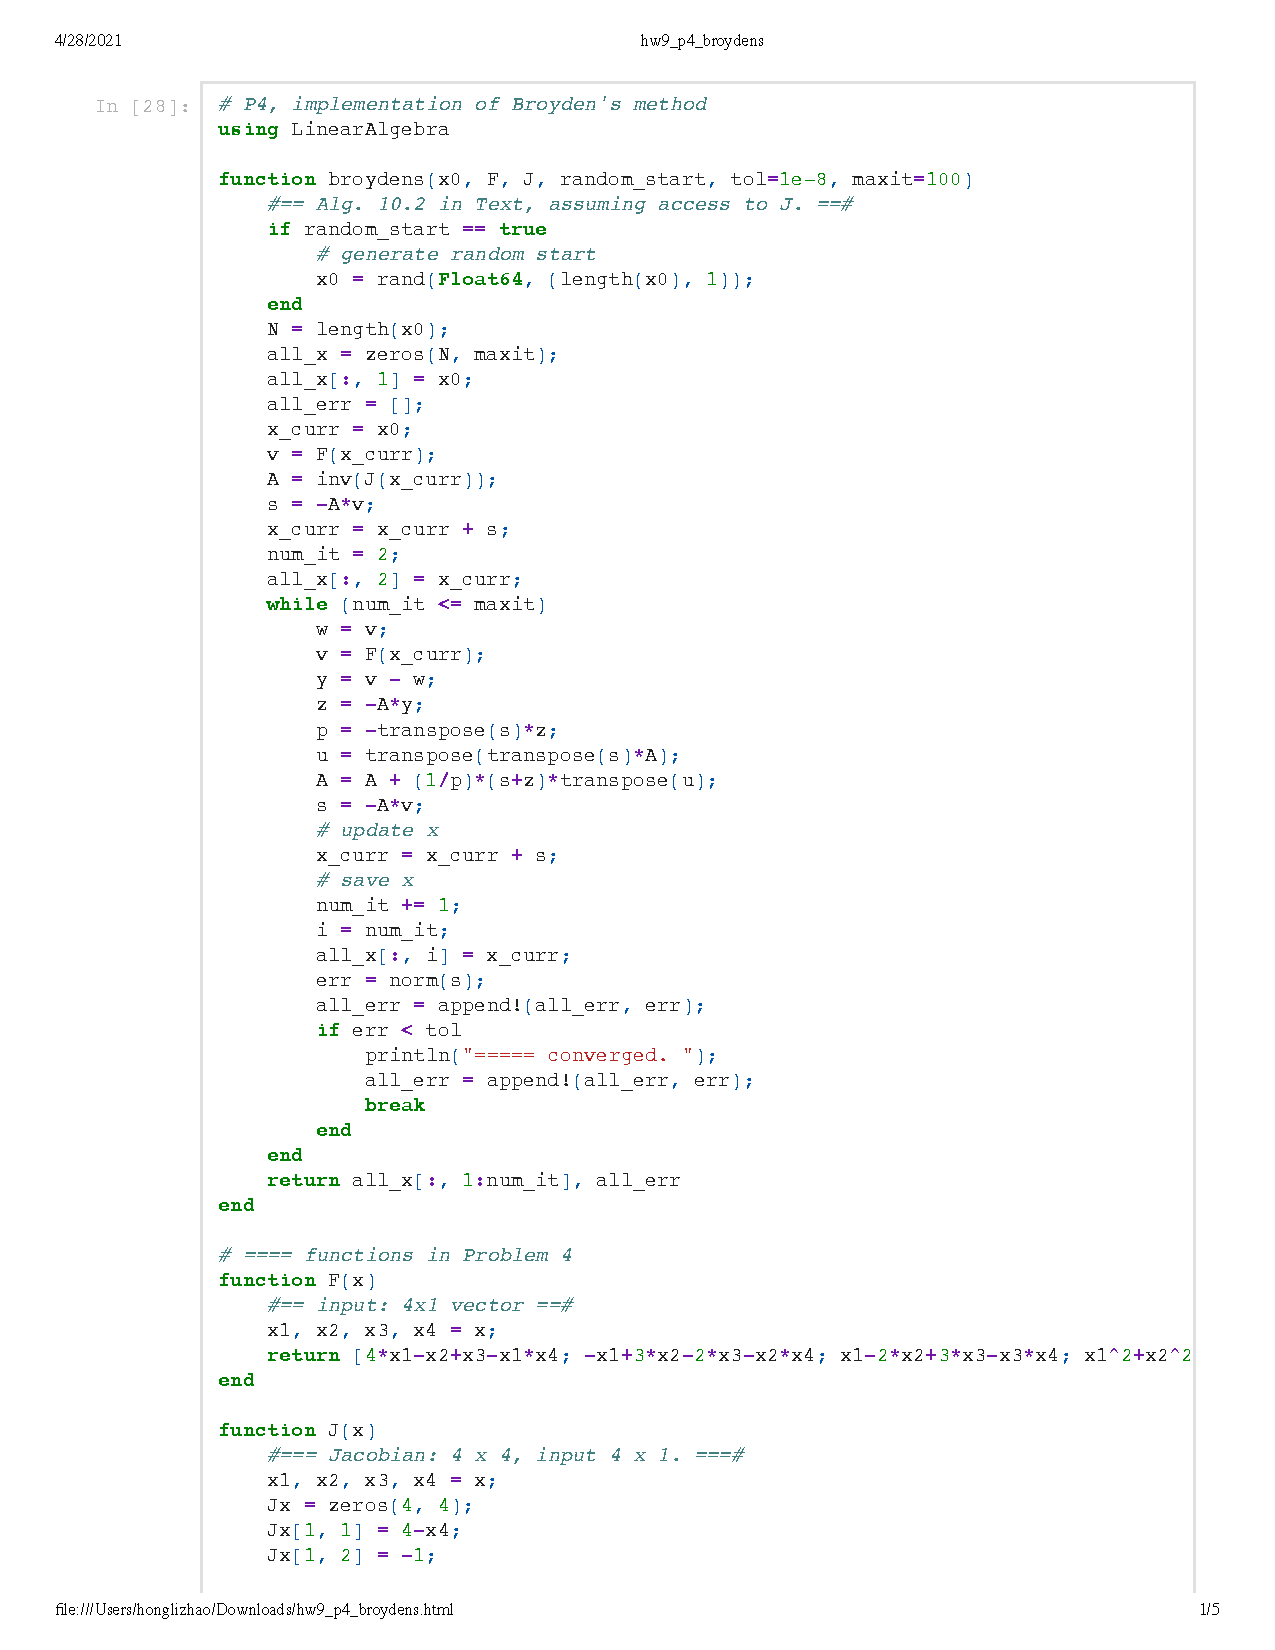
\includepdf[pages=-]{hw9_p4_broydens.pdf}

\newpage
% begin HW10
\section{Course Project / Homework 10}
\emph{Note: Only partial solutions were published.}
\subsection{Nonlinear Shooting Algorithm}
We would like to solve the following boundary value problem:
$$
	y''(x) = -(y'(x))^2 - y(x)+\ln x, x\in [1,2]
$$
$$
	y(1) = 0, y(2) = \ln 2
$$ using nonlinear shooting with Newton's method; the method is described in Section 11.1 and 11.2 from textbook.

With uniqueness assumption (Theorem 11.1), the main idea is to convert the boundary value problem to an initial value problem, and perturbing the initial condition (the initial slope $y'$). The uniqueness constraint is important, but not a requirement for convergence of the numerical method. \href{https://www.sciencedirect.com/science/article/pii/S0898122101002504}{\color{blue}This paper} has done numerical studies of the solution behavior. Different initial conditions can yield drastically different solutions for badly behaved systems.


\subsubsection{Derivation}
We follow Textbook (11.9)-(11.13), and repeatedly solve two associated initial value problem.

At step $k$, to advance from $t_k\mapsto t_{k+1}$, we solve:

$$
\begin{cases}
	y''(x,t_k) = f(x, y, y'), y(1,t_k) = 0, y'(1,t_k) = t_k\\
	z''(x,t_k) = \frac{\partial f}{\partial y}(x,y,y')z(x,t_k) + \frac{\partial f}{\partial y'}(x,y,y')z'(x,t), z(1, t_k) = 0, z'(1, t_k) = 1
\end{cases}
$$ then Newton's method gives us the next step:
$$
	t_{k+1} = t_k - \frac{y(2, t_k) - \ln 2}{z(2, t_k)}
$$

Here in our problem, $f(x,y,y') = -(y')^2 - y + \ln x$. Then:
$$
	\frac{\partial f}{\partial y}(x,y,y') = -1
$$
$$
	\frac{\partial f}{\partial y'}(x,y,y') = -2y'
$$


At the beginning of the iteration, we initialize:
$$
	t_0 = \frac{\ln 2-0}{2-1} = \ln 2
$$

The main routine is to treat $t_k$ as a parameter, and solve the two initial value problem over $x\in [1,2]$ for each $k$. Until the solution error at $x=2$ (the right boundary) is satisfactory, we update $t_k\mapsto t_{k+1}$ via Newton's method. 

The two second order ODE (in $x$) can be re-expressed as systems of first order ODEs via the following:

$$
	w_1 = y
$$
$$
	w_2 = y'
$$
$$
	w_3 = z
$$
$$
	w_4 = z'
$$

Then we have:
$$
	{\bf{w}}'(x)=\frac{d}{dx}
	\begin{pmatrix}
		w_1(x)\\
		w_2(x)\\
		w_3(x)\\
		w_4(x)
	\end{pmatrix} = 
	\begin{pmatrix}
		w_2(x)\\
		-w_2(x)^2 - w_1(x) + \ln x\\
		w_4(x)\\
		-w_3(x) - 2w_2(x)\cdot w_4(x)
	\end{pmatrix}
$$ with the initial condition:
$$
	{\bf{w}}(1) = 
	\begin{pmatrix}
		0\\
		t_k\\
		0\\
		1
	\end{pmatrix}
$$ which can be solved by any standard numerical integrator, such as Runge-Kutta.


\subsubsection{Example Pseudocode}
In order to update $t_{k+1}$, we need to rely on $y(2,t_k), z(2, t_k)$, which are only obtained through integration over the domain $[1,2]$ using parameter $t_k$.

The algorithm is inherently sequential, as is the case in many finite difference methods. When we consider implicit methods, we will see that there is a (interesting) tradeoff between runtime and space:

(1) Solving the entire solution step by step, one point at a time; and:

(2) Solving the entire solution at once, holding many grid points at the same time.

The pseudocode is as follows:
\begin{verbatim}
initialize h, tol, t0, w0
% checks whether numerical approximation 
	at right boundary is close enough to ln2
while (|w(1) - ln2| > tol)
    w <- integrate over x=1 to x=2 using standard integrator
	    tk <- tk-1 - (w(1) - ln2) / w(3)
	    % update initial slope for next iteration
	    w(2) <- tk
end while 
\end{verbatim}
\subsubsection{Python Implementation}
In the implementation, we write our own RK4 integrator as many of us did. Student will receive full point as well if \texttt{ode45} was used (but not for solving the BVP itself). All codes are in the appendix at the end of this document. The numerical experiments were done using $h = 0.1, 0.05$ and $h = 0.01$. Approximate solutions are nearly indistinguishable from the exact solution; the error plots are at least on the order of $O(10^{-5})$, which is to be expected from the truncation error analysis of RK4.




\newpage
\subsection{Finite Difference Method with Newton's Iteration}
Please refer to section 11.3, 11.4 from Textbook for a derivation. In finite difference methods, the main idea is to assign an equally (or can be adaptive) spaced grid, and express all derivatives in terms of values on the grid via a truncated Taylor expansion. This idea is generalizable to multiple dimensions for partial derivatives. Suppose we have the function and $h$ as cell size:
$$
	f(x_1, x_2, \cdots, x_n), \text{ with appropriate smoothness properties}
$$ then the following can serve as example approximations.

Forward differencing:
$$
	\frac{\partial f}{\partial x_k} \approx \frac1h\bigg(
	f(x_1, x_2,\cdots, x_k+h, \cdots, x_n) - f(x_1, x_2,\cdots, x_k, \cdots, x_n)
	\bigg)
$$

Centered differencing:
$$
	\frac{\partial^2f}{\partial x_k^2} \approx \frac{1}{h^2}\bigg(
	f(x_1, x_2,\cdots, x_k+h, \cdots, x_n) - 2f(x_1, x_2,\cdots, x_k, \cdots, x_n) 
	$$
	$$+ f(x_1, x_2,\cdots, x_k-h, \cdots, x_n)
	\bigg)
$$

We solve the BVP by following derivation (11.20) from Textbook, which yields an implicit method. Implicit schemes are generally more stable than explicit counterparts, but are more computationally demanding (as we will need to store the entire grid in memory, along with requisite Jacobian matrices), in the sense that the initial error does not blow up to infinity; precise reasons for why they are stable can be derived through \href{https://en.wikipedia.org/wiki/Von_Neumann_stability_analysis}{\color{blue}Von Neumann Stability Analysis}.

Our problem was:
$$
	y''(x) = f(x, y, y') =  -(y'(x))^2 - y(x) + \ln x, x\in [1,2]
$$
$$
	y(1) = 0, y(2) = \ln 2
$$

As before:
$$
	f_{y}(x,y,y') = -1
$$
$$
	f_{y'}(x,y,y') = -2y'
$$

Detailed derivation can be found from textbook. For Newton's iteration, we follow Algorithm 11.4. At step 0, we initialize a linear approximation; this choice of initial vector serves as a good guess for Newton's method:
$$
	\bf{w}^{(0)} = 
	\begin{pmatrix}
	\alpha\\
	\alpha + \frac{\beta-\alpha}{b-a}h\\
	\alpha + 2\frac{\beta-\alpha}{b-a}h\\
	\vdots\\
	\alpha + N\frac{\beta-\alpha}{b-a}h\\
	\beta
	\end{pmatrix}
$$

And the tridiagonal Jacobian matrix for each iteration is:
$$
	\bf{J}(\bf{w^{(k)}}) = 
	\begin{cases}
		-1 + \frac12hf_{y'}(x_i, w_i, w_i'), \text{ upper diagonal}\\
		2 + h^2f_y(x_i, w_i, w_i'), \text{ diagonal}\\
		-1 - \frac12hf_{y'}(x_i, w_i, w_i'), \text{ lower diagonal}
	\end{cases}
	$$
	$$ = 
	\begin{cases}
		-1 - hw_i', \text{ upper diagonal}\\
		2 - h^2, \text{ diagonal}\\
		-1 + hw_i', \text{ lower diagonal}
	\end{cases}
$$ where $w_i'$ is approximated using centered differencing, namely:
$$
	w_{i}' = \frac{w_{i+1} - w_{i-1}}{2h}
$$

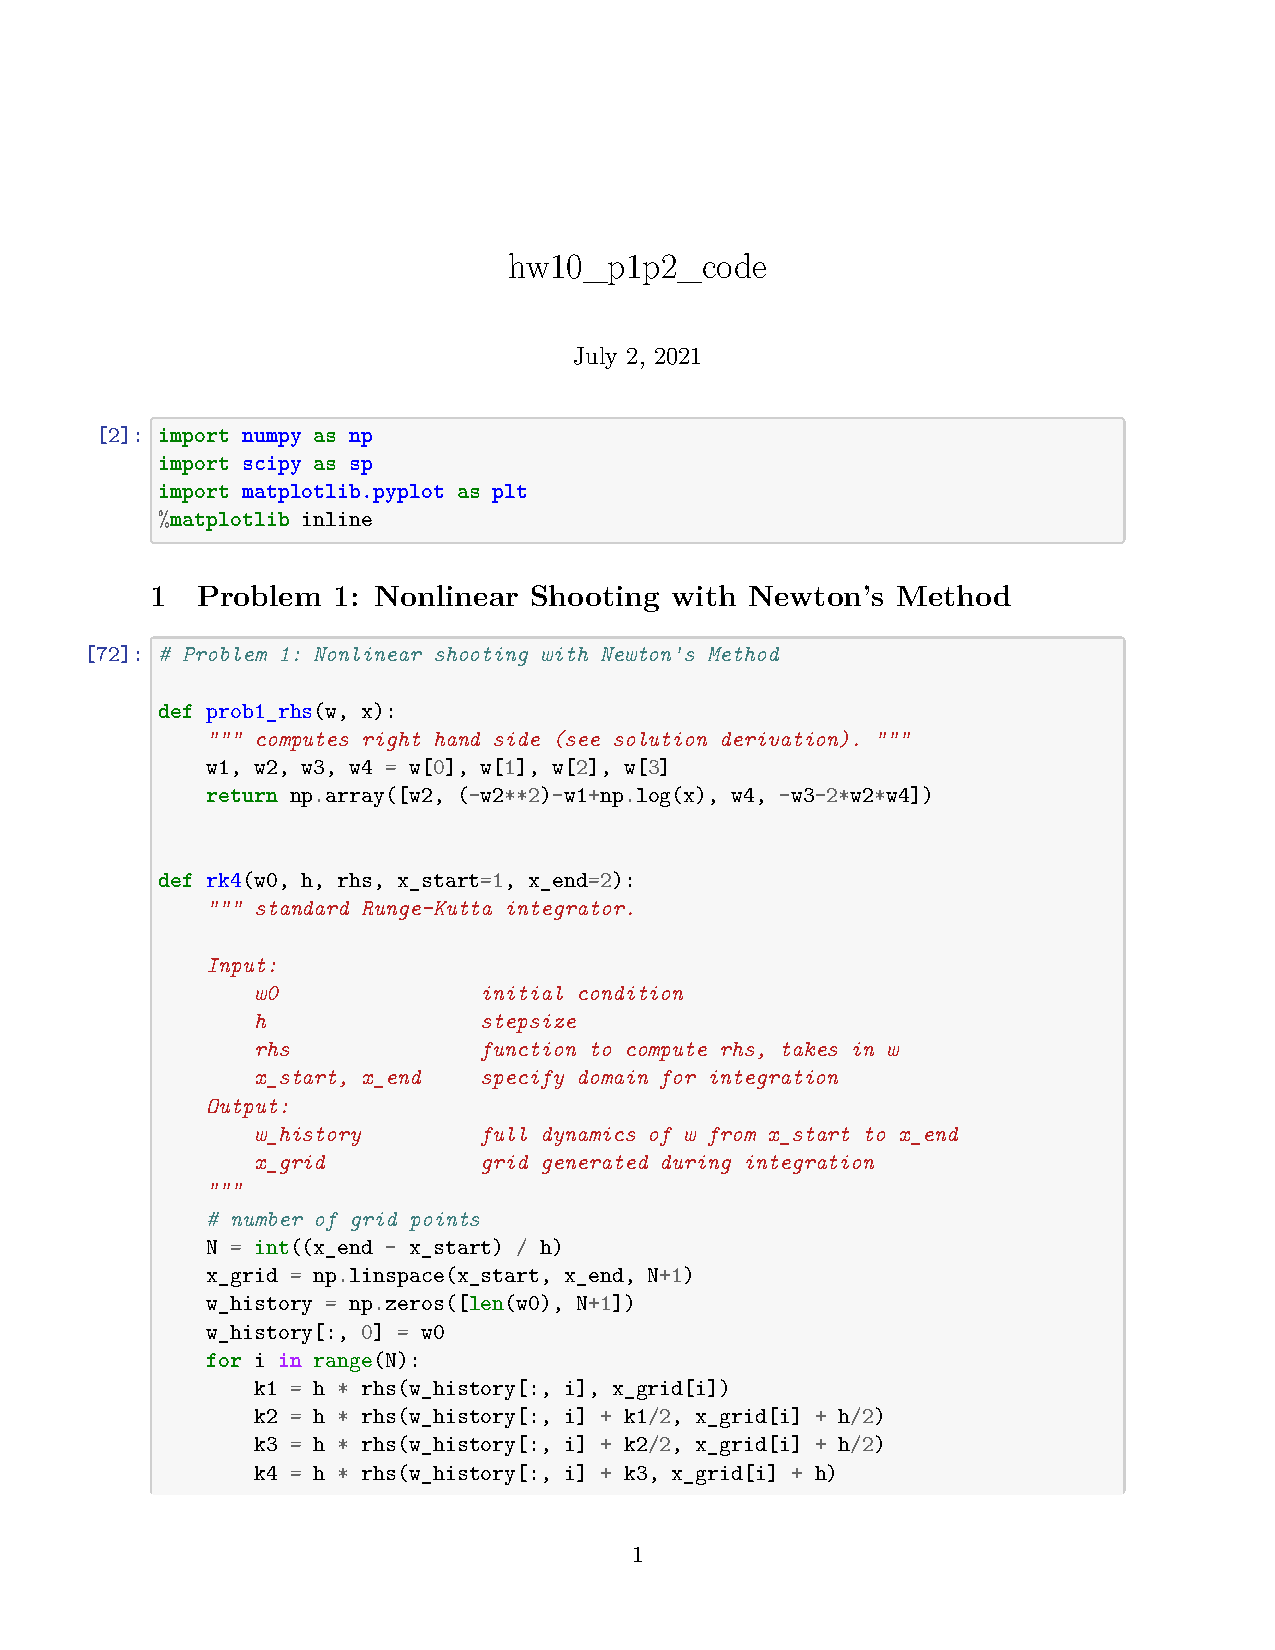
\includepdf[pages=-,scale=2,pagecommand={},width=\textwidth,linktodoc=true]{hw10_p1p2_code.pdf}

We used step sizes $h = 0.1, 0.05, 0.01$. We expect this method to be at least second order.

\subsection{Further Problems}
Due to time constraint, solutions to the rest of the project were not published. One may attempt the following problems, please send an email to any of the course staff members if interested.
\subsubsection{Implementation of Poisson Equation Finite-Difference Method and Solve B\& F Page 742, Problem 3}
\subsubsection{Implementation of Crank-Nicholson Method, and Solve B\& F Page 754, Problem 2}
\subsubsection{Implementation of the Wave Equation using Finite-Difference Method, and Solve B\& F Page 763, Problem 2}












% begin Final Exam
\newpage
\section{Final Exam, Spring 2021}
\begin{abstract}
	\emph{This document serves as reference solutions for Math 128B, Spring 2021 by Prof.Olga Holtz. The final was held online via the Gradescope platform, Thursday, May 13th, 2021, from 3:10 pm to 6:25 pm. Please find solutions after the final exam.}
\end{abstract}


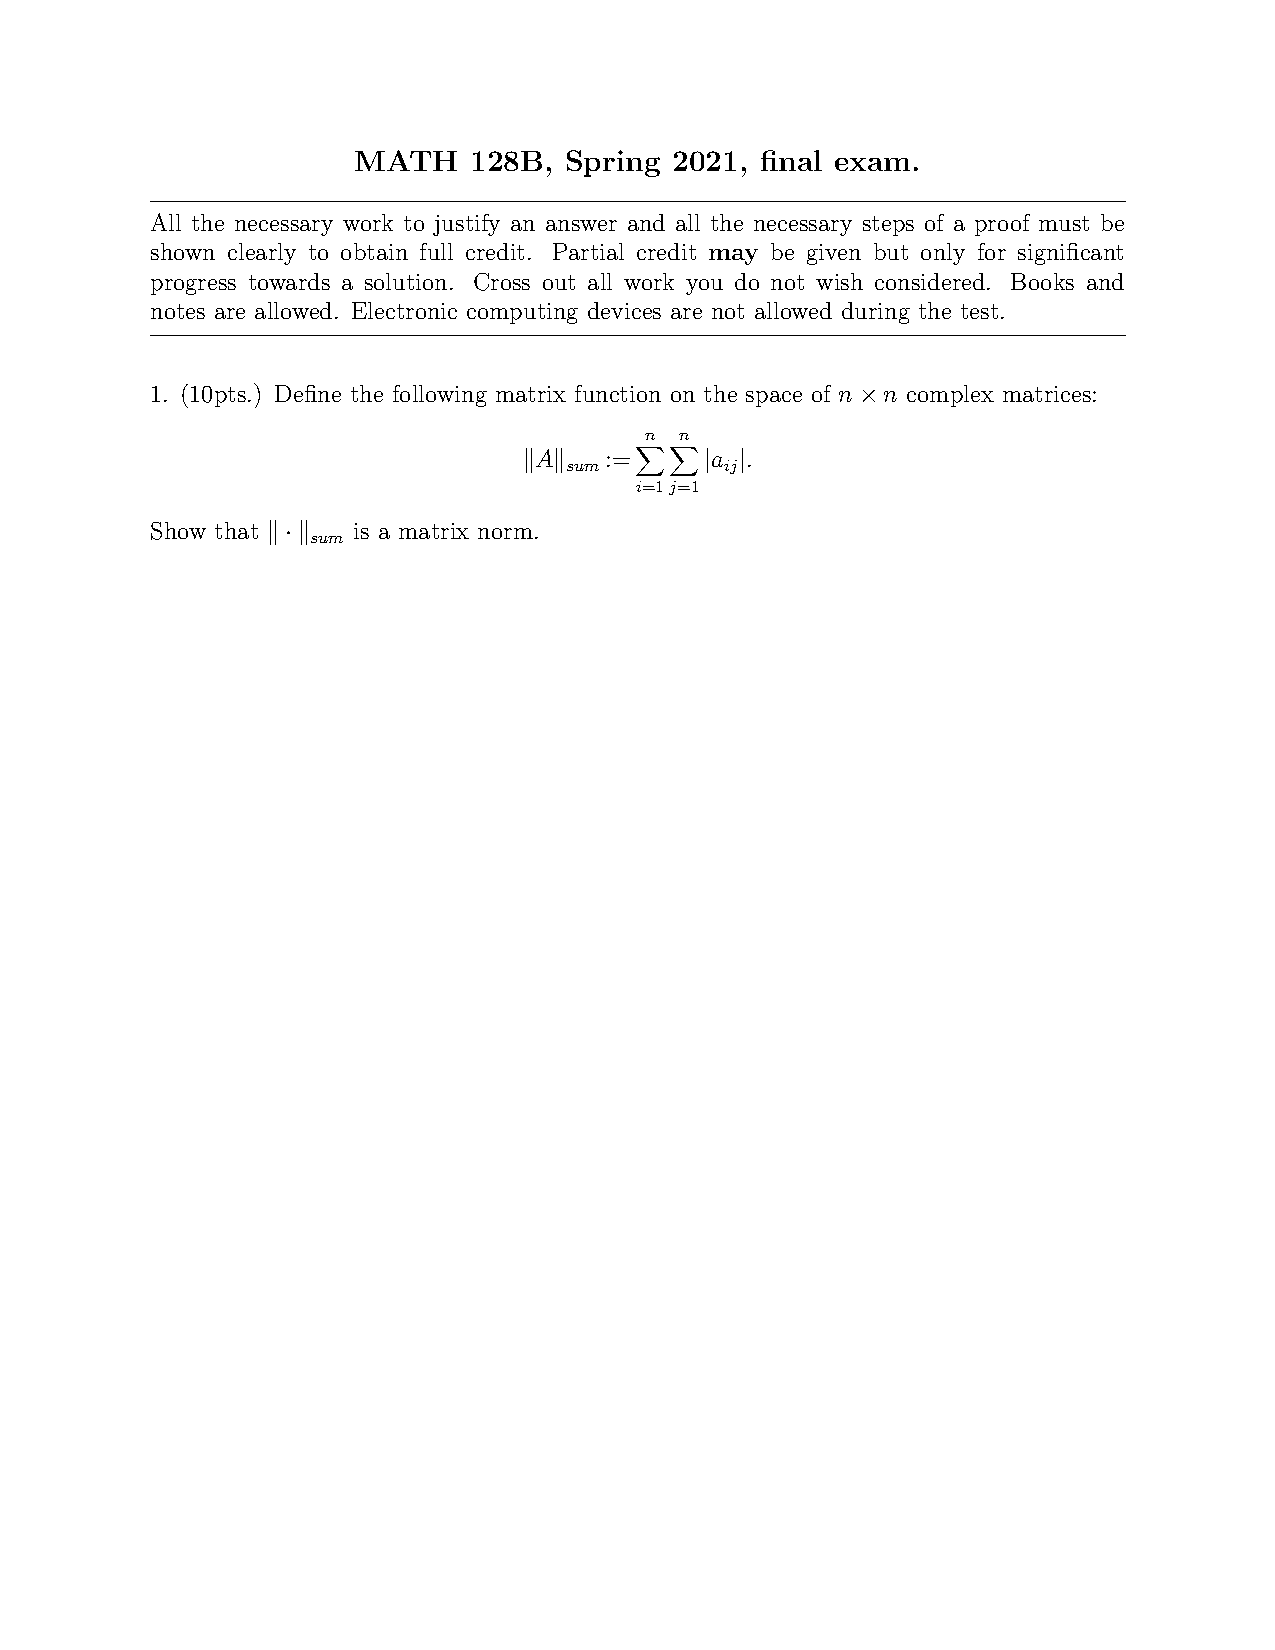
\includepdf[pages=-,scale=10,pagecommand={},width=\textwidth,linktodoc=true]{final_2021.pdf}

Begin Solution:
\subsection{Matrix Norm}
Following Definition 7.8 in textbook, a matrix norm on the space of $n\times n$ complex matrices need to satisfy:

(1) (Positivity) $\norm{A} \ge 0$, and $\norm{A} = 0$ if and only if $A=0$.

(2) (Homogeneous) $\norm{\alpha A} = \abs{\alpha}\cdot\norm{A}$ for all $\alpha\in \cc$.

(3) (Triangle inequality) $\norm{A+B} \le \norm{A} + \norm{B}$.

(4) (Sub-multiplicative) $\norm{AB} \le \norm{A}\cdot\norm{B}$.

The norm in question is in fact the $p$-norm ($p\in [1,\infty]$), defined as the following:
$$
	\norm{A}_p = \bigg(\sum_{i=1}^{n}\sum_{j=1}^{n}\abs{A_{ij}}^p\bigg)^{1/p}
$$

We show the above properties for the $p$-norm.

(1) Positivity is clear from the property of absolute value. $\abs{A_{ij}}\ge 0$ for all $i,j$. Furthermore, the double sum equals to 0 if and only if every entry of $A$ is 0.

(2) Homogeneity also comes from properties of absolute value. Take $\alpha\in \cc$, we have:
$$
	\norm{\alpha A}_p^p = \sum_{i=1}^n\sum_{j=1}^n\abs{\alpha A_{ij}}^p = \sum_{i=1}^n\sum_{j=1}^n\abs{\alpha}^p\cdot\abs{A_{ij}}^p = \abs{\alpha}^p\sum_{i=1}^n\sum_{j=1}^n\abs{A_{ij}}^p = \abs{\alpha}^p\cdot\norm{A}_p^{p}
$$

(3) Triangle inequality: Take $A,B\in\cc^{n\times n}$, then:
$$
	\norm{A+B}_p^p = \sum_{i=1}^n\sum_{j=1}^n\abs{A_{ij} + B_{ij}}^p \le \sum_{i=1}^n\sum_{j=1}^n (\abs{A_{ij}} + \abs{B_{ij}})^p
$$ and we can conclude the inequality by noting:
$$
	(\abs{A_{ij}} + \abs{B_{ij}})^p \le \abs{A_{ij}}^p + \abs{B_{ij}}^p
$$ for all $i,j$. However, this may not be immediately obvious. For $p=1$, it is triangle inequality of absolute values. For other $p$'s, one can attempt to prove:
$$
	(1+t)^p \le 1+t^p
$$ where we take $\abs{A_{ij}} = 1$, $t=\frac{\abs{B_{ij}}}{\abs{A_{ij}}}$. We can assume $\abs{A_{ij}} = 1$ without loss of generality, because:
$$
	(a+b)^p = {a^p}(1+\frac{b}{a})^p
$$ and scaling is proved from above. The rest of the proof is generally a fact and can be found in standard textbooks in real analysis or numerical analysis.

(4) Take $A,B\in\cc^{n\times n}$, then:
$$
	\norm{AB}_p^p = \sum_{i=1}^n\sum_{j=1}^n\abs{\sum_{k=1}^nA_{ik}B_{kj}}^p \le \sum_{i=1}^n\sum_{j=1}^n\sum_{k=1}^n \abs{A_{ik}}^p\abs{B_{kj}}^p
$$ since this triple sum is finite, we can exchange summation orders:
$$
	= \sum_{i=1}^n\sum_{k=1}^n\sum_{j=1}^n \abs{A_{ik}}^p\abs{B_{kj}}^p 
	$$
	$$= \sum_{i=1}^n\sum_{k=1}^n\abs{A_{ik}}^p \sum_{j=1}^n\abs{B_{kj}}^p \le \bigg(
	\sum_{i=1}^n\sum_{k=1}^n\abs{A_{ik}}^p
	\bigg)\cdot
	\bigg(
	\sum_{k=1}^n\sum_{j=1}^n\abs{B_{kj}}^p
	\bigg) = \norm{A}_p^p\cdot\norm{B}_p^p
$$



\newpage
\subsection{Orthonormal Polynomials}
The closed form for Legendre polynomials are defined as:
$$
	P_n(x) = \frac{(n+\frac12)^{1/2}}{2^nn!}\frac{d^n}{dx^n}(x^2-1)^n
$$

We follow Definition 8.5 about orthonormal polynomials with $w = 1$, on the interval $[-1,1]$, using integration by parts. Without loss of generality assume $m\ge n$. For simplicity, write $c_k = \frac{(k+1/2)^{1/2}}{2^kk!}$.
$$
	\int_{-1}^1P_m(x)P_n(x)dx = \int_{-1}^1 c_mc_n\bigg(\frac{d^m}{dx^m}(x^2-1)^m\bigg)\bigg(\frac{d^n}{dx^n}(x^2-1)^n\bigg)dx
$$ a common solution is to use integration by parts to compute:
$$
	\int_{-1}^1\bigg(
	\frac{d^m}{dx^m}(x^2-1)^m
	\bigg)
	\bigg(
	\frac{d^n}{dx^n}(x^2-1)^n
	\bigg)dx = \bigg(
	\frac{d^n}{dx^n}(x^2-1)^n
	\bigg)\cdot \bigg(
	\frac{d^{m-1}}{dx^{m-1}}(x^2-1)^m
	\bigg)\bigg|_{-1}^1 
$$
$$
	- \int_{-1}^1\bigg(
	\frac{d^{m-1}}{dx^{m-1}}(x^2-1)^m
	\bigg) \cdot \bigg(
	\frac{d^{n+1}}{dx^{n+1}}(x^2-1)^n
	\bigg) dx
$$

We have that the boundary term vanishes, by considering the latter factor:
$$
	\frac{d^{m-1}}{dx^{m-1}}(x^2-1)^m = \frac{d^{m-1}}{dx^{m-1}}(x+1)^m(x-1)^m
$$ by repeatedly applying product rule, one can show inductively that the final expression involves a sum of products of $(x+1)^k$ and $(x-1)^k$ for $k\ge 1, k\in \nn$. And hence at either $x=-1$ or $x=1$, the expression vanishes identically.

Proceeding with integration by parts on:
$$
	\int_{-1}^1\bigg(
	\frac{d^m}{dx^m}(x^2-1)^m
	\bigg)
	\bigg(
	\frac{d^n}{dx^n}(x^2-1)^n
	\bigg)dx = -\int_{-1}^1\bigg(
	\frac{d^{m-1}}{dx^{m-1}}(x^2-1)^m
	\bigg)\bigg(
	\frac{d^{n+1}}{dx^{n+1}}(x^2-1)^n
	\bigg) dx
$$ for $(m-1)$ more times, we eventually obtain:
$$
	= (-1)^m\int_{-1}^1 (x^2-1)^m \bigg(
	\frac{d^{n+m}}{dx^{n+m}}(x^2-1)^n
	\bigg)dx
$$ now since $m\ge n$ by assumption, then $n+m\ge 2n$.

If $m\neq n$, $n+m\ge 2n+1$, and $(x^2-1)^n$ is a degree $2n$ polynomial, hence the derivative:
$$
	\frac{d^{n+m}}{dx^{n+m}}(x^2-1)^n= 0
$$ this shows:
$$
	\int_{-1}^1P_m(x)\cdot P_n(x)dx = 0
$$

If $m=n$, we have:
$$
	\int_{-1}^1P_n^2(x)dx = (-1)^n(2n)!c_n^2\int_{-1}^1(x^2-1)^ndx
$$ the factorial term is from:
$$
	\frac{d^{2n}}{dx^{2n}}\big[x^{2n}+O(x^{2n-1})\big] = (2n)!
$$

There are certain ways to compute the integral $\int_{-1}^1(x^2-1)^ndx$, based on the difficulty and student responses, students received full credit if:

(1) Student looked up what is referred to as "Gamma function" from other standard textbooks.

(2) Student used integration by parts to directly evaluate:
$$
	\int_{-1}^1(x^2-1)^ndx = (-1)^n\int_{-1}^1(1-x^2)^ndx
$$ recursively, while making note that boundary terms vanish on $[-1,1]$.

(3) Student left the un-simplied expression as-is, while documenting fully correct other coefficients.

(4) Student did not choose to evaluate $m=n$ by integration by parts but used instead the recurrence relation of Legendre polynomials.

In the end:
$$
	(-1)^n\int_{-1}^1(x^2-1)dx=\frac{n!}{(n+\frac12)(n-\frac12)(n-\frac{3}{2})\cdots \frac12}
$$

And:
$$
	\int_{-1}^1P_n^2(x)dx = (2n)!\cdot\frac{(n+\frac12)}{2^{2n}(n!)^2}\cdot \frac{n!}{(n+\frac12)(n-\frac12)(n-\frac{3}{2})\cdots \frac12}
$$
$$
	= \frac{(2n)!}{2^{2n}n!(n-\frac12)(n-\frac32)\cdot\frac12} =1
$$ the last equality comes from distributing $2^n = 2\cdot 2\cdot 2\cdots 2$ to each term $n-\frac12$, $n-\frac32$ $\cdots$, $\frac12$ to yield $(2n-1)(2n-3)(2n-5)\cdots 1$. The even terms comes from $2^nn!$ in a similar manner.



\newpage
\subsection{Trigonometric Interpolation}
\subsubsection{(a) Solve for $c_j$}
\emph{Comment: }Relies on the fact that $\{e^{ijk\pi/n}\}$ forms an orthogonal set. 

We directly expand the sum.
$$
	\sum_{k=-n}^n{'}f(x_k)e^{-ijx_k}
$$ here $j$ is a fixed index, and is not meant to be confused with a dummy index for expressing summation, here we substitute in:
$$
	f(x_k) = \sum_{l=-n}^{n}{'}c_le^{ilx_k}
$$ and we have:
$$
	\sum_{k=-n}^{n}{'}\bigg(\sum_{l=-n}^n{'}c_le^{ilx_k}\bigg)e^{-ijx_k} = \sum_{k=-n}^{n}{'}\bigg(\sum_{l=-n}^n{'}c_le^{i(l-j)x_k}\bigg)
$$ now we observe that $e^{i(l-j)x_k} = \delta_{l,j}$ for $x_k$ equally spaced, where $\delta_{l,j} = 1$ only when $l=j$, by orthogonality. Hence only $c_j$ will survive in the summation, and we have:
$$
	= \sum_{k=-n}^n{'}c_j = (2n+1-1)c_j = 2nc_j
$$ since $c_j$ does not depend on $k$ (the sum has $(2n+1)$ terms, namely $-n, -n+1, \cdots, -1$ are $n$ terms; $1, 2, \cdots, n$ are $n$ terms; $k=0$ is an additional term that some students missed). The endpoints $\pm n$ agree for all nodes $x_k$.

Now divide both sides by $2n$, we yield the desired result.

\subsubsection{(b) Parseval's Theorem}
The problem is showing the discrete version of Parseval's theorem, which states that (discrete) Fourier transform is a unitary transformation (in the sense that it preserves the squared norm).

This is done by directly making use of any / all of the following:

(1) Part (a).

(2) Orthogonal set $\{e^{ijx_k}\}$.

(3) Complex exponential has unit absolute value.

(4) $\abs{z}^2 = z\cdot \overline{z}$ where $\overline{z}$ denotes the complex conjugate.

$$
	\sum_{k=-n}^n{'}\abs{f(x_k)}^2 = \sum_{k=-n}^n{'}f(x_k)\cdot\overline{f(x_k)}
$$
$$
	= \sum_{k=-n}^n{'}\bigg(
	\sum_{j=-n}^n{'}c_je^{ijkx_k}
	\bigg)\cdot
	\bigg(
	\sum_{l=-n}^n{'}\overline{c_j}\cdot e^{-ilx_k}
	\bigg)
$$ with similar reasoning, only the diagonal terms will survive from the inner distribution:
$$
	= \sum_{k=-n}^n{'}\sum_{j=l=-n}^{n}{'}c_j\cdot\overline{c_j} = \sum_{k=-n}^n{'}\sum_{j=-n}^n{'}\abs{c_j}^2
$$ exchanging the summation and noting that $c_j$ has no dependence on $k$ yields:
$$
	= \sum_{j=-n}^n{'}(2n+1-1)\abs{c_j}^2 = 2n\sum_{j=-n}^n{'}\abs{c_j}^2
$$ as desired.
\newpage
\subsection{Unique Numerical Solution for Linear BVP}
From (11.19) in textbook, we remember the linear system was formulated by using centered differencing to replace $y'' = \frac{d^2}{dx^2}y\approx \frac{1}{h^2}(y_{i+1} - 2y_i+ y_{i-1})$ and $y' = \frac{d}{dx}y \approx \frac{1}{2h}(y_{i+1}-  y_{i-1})$, yielding the following tridiagonal system:
$$
	\begin{pmatrix}
	2+h^2q(x_1) & -1+\frac{h}{2}p(x_1) & 0 & \cdots & 0 \\
	-1-\frac{h}{2}p(x_2) & 2+h^2q(x_2) & -1 + \frac{h}{2}p(x_2) & \cdots & \vdots\\
	0 & \ddots & \ddots & \ddots & 0 \\
	\vdots & \ddots & \ddots & \ddots & -1+\frac{h}{2}p(x_{N-1}) \\
	0 & \cdots & \cdots & -1-\frac{h}{2}p(x_N) & 2+h^2q(x_N)
	\end{pmatrix}\bf{y} = \bf{b}
$$ the problem amounts to showing that the tridiagonal system is nonsingular; under the condition that:
$$
	h < \frac{2}{L} = \frac{2}{\max_{x\in[a,b]}\abs{p(x)}}, q(x)\ge 0
$$ 

Furthermore, a matrix is nonsingular if and only $0$ is not an eigenvalue; we have thus converted this problem into an eigenvalue estimation problem, where we exploit Gershgorin's Theorem. 

We have an estimate of the size:
$$
	\abs{\frac{h}{2}p(x)} \le \frac{h}{2}L < \frac{L}{2}\cdot \frac{2}{L} = 1
$$ therefore:
$$
	\abs{-1-\frac{h}{2}p(x)} = \abs{-(1+\frac{h}{2}p(x))} = 1+\frac{h}{2}p(x)
$$ because $\frac{h}{2}p(x)$ has magnitude strictly less than 1, the quantity is guaranteed to be negative. Similarly:
$$
	\abs{-1+\frac{h}{2}p(x)} = 1-\frac{h}{2}p(x)
$$

Gershgorin's theorem states that:
$$
	\lambda \in \bigcup_{i=1}^NR_i
$$ where:
$$
	R_i = \big\{
	z\in\cc, \abs{z-A_{ii}}\le \sum_{j=1,j\neq i}^N\abs{A_{ij}}
	\big\}
$$ where $A$ is our tridiagonal matrix. 

For all $i=2,3,\cdots, N-1$:
$$
	R_i = \{z\in\cc, \abs{z-\bigg(2+h^2q(x_i)\bigg)}\le \abs{-1-\frac{h}{2}p(x_i)} + \abs{-1+\frac{h}{2}p(x_i)}\}
$$

By above arguments, we know that:
$$
	\abs{-1-\frac{h}{2}p(x_i)} + \abs{-1+\frac{h}{2}p(x_i)} = 1+1 = 2
$$

Then the circles became:
$$
	R_i = \{z\in\cc: \abs{z-(2+h^2q(x_i))} \le 2\}
$$ we solve for $z$ in $R_i$ for all $i\in\{2,3,\cdots, N-1\}$:
$$
	0\le h^2q(x_i)\le z\le 4+h^2q(x_i)
$$

At the boundaries, namely $i=1$ or $i=N$, we have:
$$
	R_i = \{z\in \cc: \abs{z-(2+h^2q(x_i))} \le 1\pm \frac{h}{2}p(x)\}
$$

By triangle inequality:
$$
	\abs{-1\pm \frac{h}{2}p(x)} \le 1 + \frac{h}{2}\abs{p(x)} < 2
$$ then we solve for $z\in R_1, R_N$:
$$
	 0\le h^2q(x_i)< z < 4+h^2q(x_i)
$$

\emph{Comment:} One can stop here, conclude that the tridiagonal matrix is weakly diagonally dominant and refer to Theorem 6.31 to conclude that the tridiagonal system is nonsingular. More precisely, Gersgorin's theorem may not yield the desired tight bound even $q=0$ is allowed. Student solutions that directly applied Gersgorin's theorem without coping with this subtlety are (tentatively) given full credit.

\newpage
\subsection{Power Method}
We follow the inductive definition of (9.3) inductively from textbook, where:
$$
	y^{(m)} = Ax^{(m-1)} 
$$ which is normalized with respect to $\norm{\cdot}_{\infty}$ after each step:
$$
	x^{(m)} = \frac{y^{(m)}}{\norm{y^{(m)}}_{\infty}}
$$ yielding (inductively, student solution can direct refer to this expression without establishing $\mu^{(1)}$):
$$
	\mu^{(m)} = \frac{\sum_{i=1}^n\alpha_i\lambda_i^m v^{(i)}_{p_{m-1}}}{\sum_{i=1}^n\alpha_i\lambda_i^{m-1} v^{(i)}_{p_{m-1}}}
$$ where $p_{m-1}$ is the index such that $x^{(m-1)}_{p_{m-1}} = \norm{x}_{\infty}$. Regardless of the specific $p$, $v_{p_{m-1}}^{(i)}$ is a scalar.

Recall that this is done by iteratively considering:
$$
	Ax^{(0)} = A(\sum_{i=1}^n\alpha_iv^{(i)}) = \sum_{i=1}^n\alpha_iAv^{(i)} = \sum_{i=1}^n\alpha_i\lambda_iv^{(i)}
$$ where $v^{(i)}$ is an eigenvector with eigenvalue $\lambda_i$, hence the last equality.

In our case, $\alpha_1 = 0$, then we can rewrite:
$$
	\mu^{(m)} = \frac{\alpha_2\lambda_2^mv_{p_{m-1}}^{(2)}+\sum_{i=3}^n \alpha_i\lambda_i^mv_{p_{m-1}}^{(i)}}{\alpha_2\lambda_2^{m-1}v_{p_{m-1}}^{(2)}+\sum_{i=3}^n \alpha_i\lambda_i^{m-1}v_{p_{m-1}}^{(i)}} = \lambda_2\bigg(
	\frac{\alpha_2v_{p_{m-1}}^{(2)} + \sum_{i=3}^n\alpha_i\big(\frac{\lambda_i}{\lambda_2}\big)^{m}v_{p_{m-1}}^{(i)}}{\alpha_2v_{p_{m-1}}^{(2)} + \sum_{i=3}^n\alpha_i\big(\frac{\lambda_i}{\lambda_2}\big)^{m-1}v_{p_{m-1}}^{(i)}}
	\bigg)
$$

Since the eigenvalues are sorted, $\abs{\frac{\lambda_i}{\lambda_2}} < 1$, we have for all $i > 2$:
$$
	\ntoinf{m}\bigg(
	\frac{\lambda_i}{\lambda_2}
	\bigg)^m = 0
$$

Taking the limit of $\mu^{(m)}$ yields:
$$
	\ntoinf{m}\mu^{(m)} = \lambda_2
$$

\newpage
\subsection{Householder Transformation and Givens Rotation Equivalence}
Intuitively we would expect the answer to be no. A givens rotation:
$$
	R(\theta) = 
	\begin{pmatrix}
		\cos(\theta) & -\sin(\theta)\\
		\sin(\theta) & \cos(\theta)
	\end{pmatrix}
$$ rotates any vector $v\in \rr^2$ counterclockwise by $\theta$. In 3 dimensions $(x,y,z)$ coordinates, we can choose to embed this rotation for any pair of indices. We can choose to rotate on the plane $(x,y),(x,z)$ and $(y,z)$ by $\theta$ degree, counterclockwise. On the other hand, householder reflection $P = I - 2uu^T$, applied on some vector $v$, where $u = e_1$ is a reflection of $v$ in the (hyper)plane through 0 and perpendicular to $e_1$. If $e_1$ is unit vector on the $x$-axis in $\rr^2$, then in 2D specifically, $P$ would be a reflection across the $y$-axis. In the simplest 2D case, we see intuitively that there are at least 2 ways to rotate $v$ using Givens rotation such that it matches $Pv$ eventually (in higher dimensions, there are many more ways to rotate than to reflect); namely clockwise ($\theta<0$) and counterclockwise ($\theta>0$). The  rotation matrix is not equal to a reflection matrix.

\emph{Counterexample (2D)}
Let $v=[1,0]^T=e_1$, $u = e_2 = [0,1]^T$, and then:
$$
	P = I-2uu^T =
	\begin{pmatrix}
		1 & 0\\
		0 & -1
	\end{pmatrix}
$$ this can be considered as a reflection across the $x$-axis, trivially:
$$
	Pv = \begin{pmatrix}
		1 & 0\\
		0 & -1
	\end{pmatrix}\begin{pmatrix}1\\0 \end{pmatrix}=
	\begin{pmatrix}1\\0 \end{pmatrix}
$$

The same can be achieved by the counterclockwise (Givens) rotation in the $(x,y)$ plane by $0$ or $2\pi$ degrees, let:
$$
	R(2\pi) = \begin{pmatrix}
		\cos(2\pi) & -\sin(2\pi)\\
		\sin(2\pi) & \cos(2\pi)
	\end{pmatrix} =
	\begin{pmatrix}
		1 & 0\\
		0 & 1
	\end{pmatrix}
$$

$$
	Rv = Iv = v
$$ but $R\neq P$. In both of these cases $Rv=Pv = \norm{v}_2e_1$.

\section{Concluding Remarks}

\hspace{3ex} I have always had a special feeling towards numerical analysis. Using algorithms to perform mathematical and statistical computations to test ideas, and observing our pure mathematicians making correct predictions based on rigorous theory - the whole process is simply fascinating to me, and not all feelings can be best captured by words, needless to mention not all feelings require any (pretentious) explanations. I would like to thank Prof. Olga Holtz for teaching a great course from which I had the wonderful opportunity to write up these solutions and receive feedbacks, and her mentorship to undergraduate research outside of class. 

This document is hopefully dedicated to anyone who enjoys the subject of numerical analysis. If you are a young professional who shares a similar passion, please check out Berkeley courses Math 228A, Math 228B, Math 221, STAT 243 from the Math and Stats departments; Math 202A, Math 202B, Math 222A, Math 222B for rigorous theoretical backgrounds, and COMPSCI 289A, COMPSCI 267 at EECS, as I am sure you will not regret. 

\section{Referenece}
\
\hspace{3ex} Burden, R. L., Faires, J. D., \& Burden, A. M. (2016). \emph{Numerical analysis}.

\

Demmel, J. (1997). \emph{Applied Numerical Linear Algebra}. Society for Industrial and Applied Mathematics.


























































% ================ end file
\end{document}

